\documentclass[twoside]{book}

% Packages required by doxygen
\usepackage{calc}
\usepackage{doxygen}
\usepackage{graphicx}
\usepackage[utf8]{inputenc}
\usepackage{makeidx}
\usepackage{multicol}
\usepackage{multirow}
\usepackage{textcomp}
\usepackage[table]{xcolor}

% Font selection
\usepackage[T1]{fontenc}
\usepackage{mathptmx}
\usepackage[scaled=.90]{helvet}
\usepackage{courier}
\usepackage{amssymb}
\usepackage{sectsty}
\renewcommand{\familydefault}{\sfdefault}
\allsectionsfont{%
  \fontseries{bc}\selectfont%
  \color{darkgray}%
}
\renewcommand{\DoxyLabelFont}{%
  \fontseries{bc}\selectfont%
  \color{darkgray}%
}

% Page & text layout
\usepackage{geometry}
\geometry{%
  a4paper,%
  top=2.5cm,%
  bottom=2.5cm,%
  left=2.5cm,%
  right=2.5cm%
}
\tolerance=750
\hfuzz=15pt
\hbadness=750
\setlength{\emergencystretch}{15pt}
\setlength{\parindent}{0cm}
\setlength{\parskip}{0.2cm}
\makeatletter
\renewcommand{\paragraph}{%
  \@startsection{paragraph}{4}{0ex}{-1.0ex}{1.0ex}{%
    \normalfont\normalsize\bfseries\SS@parafont%
  }%
}
\renewcommand{\subparagraph}{%
  \@startsection{subparagraph}{5}{0ex}{-1.0ex}{1.0ex}{%
    \normalfont\normalsize\bfseries\SS@subparafont%
  }%
}
\makeatother

% Headers & footers
\usepackage{fancyhdr}
\pagestyle{fancyplain}
\fancyhead[LE]{\fancyplain{}{\bfseries\thepage}}
\fancyhead[CE]{\fancyplain{}{}}
\fancyhead[RE]{\fancyplain{}{\bfseries\leftmark}}
\fancyhead[LO]{\fancyplain{}{\bfseries\rightmark}}
\fancyhead[CO]{\fancyplain{}{}}
\fancyhead[RO]{\fancyplain{}{\bfseries\thepage}}
\fancyfoot[LE]{\fancyplain{}{}}
\fancyfoot[CE]{\fancyplain{}{}}
\fancyfoot[RE]{\fancyplain{}{\bfseries\scriptsize Generated on Tue Sep 17 2013 20:07:27 for Group Modeling App by Doxygen }}
\fancyfoot[LO]{\fancyplain{}{\bfseries\scriptsize Generated on Tue Sep 17 2013 20:07:27 for Group Modeling App by Doxygen }}
\fancyfoot[CO]{\fancyplain{}{}}
\fancyfoot[RO]{\fancyplain{}{}}
\renewcommand{\footrulewidth}{0.4pt}
\renewcommand{\chaptermark}[1]{%
  \markboth{#1}{}%
}
\renewcommand{\sectionmark}[1]{%
  \markright{\thesection\ #1}%
}

% Indices & bibliography
\usepackage{natbib}
\usepackage[titles]{tocloft}
\setcounter{tocdepth}{3}
\setcounter{secnumdepth}{5}
\makeindex

% Hyperlinks (required, but should be loaded last)
\usepackage{ifpdf}
\ifpdf
  \usepackage[pdftex,pagebackref=true]{hyperref}
\else
  \usepackage[ps2pdf,pagebackref=true]{hyperref}
\fi
\hypersetup{%
  colorlinks=true,%
  linkcolor=blue,%
  citecolor=blue,%
  unicode%
}

% Custom commands
\newcommand{\clearemptydoublepage}{%
  \newpage{\pagestyle{empty}\cleardoublepage}%
}


%===== C O N T E N T S =====

\begin{document}

% Titlepage & ToC
\hypersetup{pageanchor=false}
\pagenumbering{roman}
\begin{titlepage}
\vspace*{7cm}
\begin{center}%
{\Large Group Modeling App }\\
\vspace*{1cm}
{\large Generated by Doxygen 1.8.4}\\
\vspace*{0.5cm}
{\small Tue Sep 17 2013 20:07:27}\\
\end{center}
\end{titlepage}
\clearemptydoublepage
\tableofcontents
\clearemptydoublepage
\pagenumbering{arabic}
\hypersetup{pageanchor=true}

%--- Begin generated contents ---
\chapter{Todo List}
\label{todo}
\hypertarget{todo}{}

\begin{DoxyRefList}
\item[\label{todo__todo000001}%
\hypertarget{todo__todo000001}{}%
Global \hyperlink{interface_component_a3d13675a50c2e37e16e1b7858e5510e4}{\mbox{[}Component generate\-I\-D\mbox{]}} ]would be nice to remove this static variable Called for every subclass instance to keep track of how many objects there are currently in the model. The main use of this method will be to generate identification numbers for newly created objects by the user. Should only be called once by the component model in the init.  
\item[\label{todo__todo000002}%
\hypertarget{todo__todo000002}{}%
Global \hyperlink{interface_component_a875d9dcfa3e019c2cf685524707e0427}{\mbox{[}Component sanitize\-String\-:\mbox{]}} ]For some reason string\-By\-Replacing\-Occurrences\-Of\-String causes Doxygen to not be able to find the .m file. So i have documentation duplicated in both files right now... Used to sanitize strings that may contain extraneous escape characters.  
\item[\label{todo__todo000003}%
\hypertarget{todo__todo000003}{}%
Global \hyperlink{interface_file_i_o_a2bb3d58ae1f0fac924e831a424e1365b}{\mbox{[}File\-I\-O import\-Model\-:\mbox{]}} ]The name of the loop being on the next line kind of a pain  
\item[\label{todo__todo000004}%
\hypertarget{todo__todo000004}{}%
Global \hyperlink{interface_variable_a4c7e0685f86eef33404c7ada436db10a}{\mbox{[}Variable create\-Variable\-Output\-String\mbox{]}} ]I do not put the extra characters vensim uses for " 
\end{DoxyRefList}
\chapter{Hierarchical Index}
\section{Class Hierarchy}
This inheritance list is sorted roughly, but not completely, alphabetically\-:\begin{DoxyCompactList}
\item \contentsline{section}{Detailed\-Help\-Section\-View\-Controller()}{\pageref{category_detailed_help_section_view_controller_07_08}}{}
\item \contentsline{section}{Help\-Section\-View\-Controller()}{\pageref{category_help_section_view_controller_07_08}}{}
\item \contentsline{section}{M\-F\-Side\-Menu\-Container\-View\-Controller()}{\pageref{category_m_f_side_menu_container_view_controller_07_08}}{}
\item \contentsline{section}{Model\-Section\-View\-Controller()}{\pageref{category_model_section_view_controller_07_08}}{}
\item N\-S\-Object\begin{DoxyCompactList}
\item \contentsline{section}{Component}{\pageref{interface_component}}{}
\begin{DoxyCompactList}
\item \contentsline{section}{Causal\-Link}{\pageref{interface_causal_link}}{}
\item \contentsline{section}{Loop}{\pageref{interface_loop}}{}
\item \contentsline{section}{Variable}{\pageref{interface_variable}}{}
\end{DoxyCompactList}
\item \contentsline{section}{Control\-Parameters}{\pageref{interface_control_parameters}}{}
\item \contentsline{section}{Default\-Parameters}{\pageref{interface_default_parameters}}{}
\item \contentsline{section}{Event}{\pageref{interface_event}}{}
\item \contentsline{section}{Event\-Logger}{\pageref{interface_event_logger}}{}
\item \contentsline{section}{File\-I\-O}{\pageref{interface_file_i_o}}{}
\item \contentsline{section}{Model}{\pageref{interface_model}}{}
\item \contentsline{section}{Reachability}{\pageref{interface_reachability}}{}
\end{DoxyCompactList}
\item $<$U\-I\-Application\-Delegate$>$\begin{DoxyCompactList}
\item \contentsline{section}{App\-Delegate}{\pageref{interface_app_delegate}}{}
\end{DoxyCompactList}
\item $<$U\-I\-Document\-Interaction\-Controller\-Delegate$>$\begin{DoxyCompactList}
\item \contentsline{section}{Model\-Section\-View\-Controller}{\pageref{interface_model_section_view_controller}}{}
\end{DoxyCompactList}
\item $<$U\-I\-Gesture\-Recognizer\-Delegate$>$\begin{DoxyCompactList}
\item \contentsline{section}{M\-F\-Side\-Menu\-Container\-View\-Controller}{\pageref{interface_m_f_side_menu_container_view_controller}}{}
\end{DoxyCompactList}
\item $<$U\-I\-Popover\-Controller\-Delegate$>$\begin{DoxyCompactList}
\item \contentsline{section}{Model\-Section\-View\-Controller}{\pageref{interface_model_section_view_controller}}{}
\end{DoxyCompactList}
\item U\-I\-Responder\begin{DoxyCompactList}
\item \contentsline{section}{App\-Delegate}{\pageref{interface_app_delegate}}{}
\end{DoxyCompactList}
\item U\-I\-Scroll\-View\begin{DoxyCompactList}
\item \contentsline{section}{Model\-Section\-View}{\pageref{interface_model_section_view}}{}
\end{DoxyCompactList}
\item $<$U\-I\-Scroll\-View\-Delegate$>$\begin{DoxyCompactList}
\item \contentsline{section}{Model\-Section\-View}{\pageref{interface_model_section_view}}{}
\end{DoxyCompactList}
\item U\-I\-Table\-View\-Controller\begin{DoxyCompactList}
\item \contentsline{section}{Help\-Section\-View\-Controller}{\pageref{interface_help_section_view_controller}}{}
\item \contentsline{section}{Side\-Menu\-View\-Controller}{\pageref{interface_side_menu_view_controller}}{}
\end{DoxyCompactList}
\item $<$U\-I\-Text\-Field\-Delegate$>$\begin{DoxyCompactList}
\item \contentsline{section}{Loop\-Edit\-Menu\-View}{\pageref{interface_loop_edit_menu_view}}{}
\item \contentsline{section}{Variable\-Edit\-Menu\-View}{\pageref{interface_variable_edit_menu_view}}{}
\end{DoxyCompactList}
\item U\-I\-View\begin{DoxyCompactList}
\item \contentsline{section}{Causal\-Link\-Edit\-Menu\-View}{\pageref{interface_causal_link_edit_menu_view}}{}
\item \contentsline{section}{Causal\-Link\-Handle\-View}{\pageref{interface_causal_link_handle_view}}{}
\item \contentsline{section}{Causal\-Link\-View}{\pageref{interface_causal_link_view}}{}
\item \contentsline{section}{Loop\-Edit\-Menu\-View}{\pageref{interface_loop_edit_menu_view}}{}
\item \contentsline{section}{Loop\-View}{\pageref{interface_loop_view}}{}
\item \contentsline{section}{New\-Causal\-Link}{\pageref{interface_new_causal_link}}{}
\item \contentsline{section}{Variable\-Edit\-Menu\-View}{\pageref{interface_variable_edit_menu_view}}{}
\item \contentsline{section}{Variable\-View}{\pageref{interface_variable_view}}{}
\end{DoxyCompactList}
\item U\-I\-View\-Controller\begin{DoxyCompactList}
\item \contentsline{section}{Detailed\-Help\-Section\-View\-Controller}{\pageref{interface_detailed_help_section_view_controller}}{}
\item \contentsline{section}{M\-F\-Side\-Menu\-Container\-View\-Controller}{\pageref{interface_m_f_side_menu_container_view_controller}}{}
\item \contentsline{section}{Model\-Section\-View\-Controller}{\pageref{interface_model_section_view_controller}}{}
\end{DoxyCompactList}
\end{DoxyCompactList}

\chapter{Data Structure Index}
\section{Data Structures}
Here are the data structures with brief descriptions\-:\begin{DoxyCompactList}
\item\contentsline{section}{\hyperlink{interface_app_delegate}{App\-Delegate} \\*The U\-I\-Responder class defines an interface for objects that respond to and handle events. It is the superclass of U\-I\-Application, U\-I\-View and its subclasses (which include U\-I\-Window). Instances of these classes are sometimes referred to as responder objects or, simply, responders }{\pageref{interface_app_delegate}}{}
\item\contentsline{section}{\hyperlink{interface_causal_link}{Causal\-Link} \\*A subclass of \hyperlink{interface_component}{Component} containing the data related to a causal link between two variables of a causal loop diagram. ex. In a diagram on Childhood obesity, there may exist a relationship between the \char`\"{}\-Fast Food Consumption\char`\"{} variable and the \char`\"{}\-Weight Gain\char`\"{} variable. This class represents that causal link }{\pageref{interface_causal_link}}{}
\item\contentsline{section}{\hyperlink{interface_causal_link_edit_menu_view}{Causal\-Link\-Edit\-Menu\-View} \\*The view that will contain the edit menu for Causal\-Links }{\pageref{interface_causal_link_edit_menu_view}}{}
\item\contentsline{section}{\hyperlink{interface_causal_link_handle_view}{Causal\-Link\-Handle\-View} \\*A view that display the vertex of the \hyperlink{interface_causal_link}{Causal\-Link}. This view is also used to move and modify the \hyperlink{interface_causal_link}{Causal\-Link} }{\pageref{interface_causal_link_handle_view}}{}
\item\contentsline{section}{\hyperlink{interface_causal_link_view}{Causal\-Link\-View} \\*A view that containg the graphical representation of a \hyperlink{interface_causal_link}{Causal\-Link} }{\pageref{interface_causal_link_view}}{}
\item\contentsline{section}{\hyperlink{interface_component}{Component} \\*A superclass that holds all generic data about all objects in the causal diagram model }{\pageref{interface_component}}{}
\item\contentsline{section}{\hyperlink{interface_control_parameters}{Control\-Parameters} \\*This class currently holds an array with the control parameters, but was created to allow for expansion if we would want to parse the array into its individual control parameters and be able to update them individually }{\pageref{interface_control_parameters}}{}
\item\contentsline{section}{\hyperlink{interface_default_parameters}{Default\-Parameters} \\*This class currently holds a string with the default parameters, but was created to allow for expansion if we would want to parse the string into its individual pieces and be able to update them individually }{\pageref{interface_default_parameters}}{}
\item\contentsline{section}{\hyperlink{interface_detailed_help_section_view_controller}{Detailed\-Help\-Section\-View\-Controller} }{\pageref{interface_detailed_help_section_view_controller}}{}
\item\contentsline{section}{\hyperlink{category_detailed_help_section_view_controller_07_08}{Detailed\-Help\-Section\-View\-Controller()} }{\pageref{category_detailed_help_section_view_controller_07_08}}{}
\item\contentsline{section}{\hyperlink{interface_event}{Event} \\*A class used to construct events that occur in the simulation }{\pageref{interface_event}}{}
\item\contentsline{section}{\hyperlink{interface_event_logger}{Event\-Logger} \\*A class used to keep a record of all of the events the user makes during a modeling session }{\pageref{interface_event_logger}}{}
\item\contentsline{section}{\hyperlink{interface_file_i_o}{File\-I\-O} \\*A class that handles the parsing of mdl files to import into the application. Also is responsible for exporting the model back into a Vensim file for saving state and for use in Vensim again }{\pageref{interface_file_i_o}}{}
\item\contentsline{section}{\hyperlink{interface_help_section_view_controller}{Help\-Section\-View\-Controller} \\*A Table view controller used to handle the help section }{\pageref{interface_help_section_view_controller}}{}
\item\contentsline{section}{\hyperlink{category_help_section_view_controller_07_08}{Help\-Section\-View\-Controller()} }{\pageref{category_help_section_view_controller_07_08}}{}
\item\contentsline{section}{\hyperlink{interface_loop}{Loop} \\*A subclass of \hyperlink{interface_component}{Component} containing the data related to a feedback loop of a causal loop diagram. ex. In a diagram on K-\/12 school attendance, a feedback loop would occur where as \char`\"{}\-Students Desire to Go to School\char`\"{} increases so does their \char`\"{}\-Mean daily attendance rate\char`\"{} and as their \char`\"{}\-Mean Daily attendance rate\char`\"{} increases so does a \char`\"{}\-Students Desire to Go to School\char`\"{} }{\pageref{interface_loop}}{}
\item\contentsline{section}{\hyperlink{interface_loop_edit_menu_view}{Loop\-Edit\-Menu\-View} \\*The view that will contain the edit menu for Loops }{\pageref{interface_loop_edit_menu_view}}{}
\item\contentsline{section}{\hyperlink{interface_loop_view}{Loop\-View} \\*A view that contains the graphical representation of a \hyperlink{interface_loop}{Loop} }{\pageref{interface_loop_view}}{}
\item\contentsline{section}{\hyperlink{interface_m_f_side_menu_container_view_controller}{M\-F\-Side\-Menu\-Container\-View\-Controller} }{\pageref{interface_m_f_side_menu_container_view_controller}}{}
\item\contentsline{section}{\hyperlink{category_m_f_side_menu_container_view_controller_07_08}{M\-F\-Side\-Menu\-Container\-View\-Controller()} }{\pageref{category_m_f_side_menu_container_view_controller_07_08}}{}
\item\contentsline{section}{\hyperlink{interface_model}{Model} \\*This class is responsible for holding all aspects of a causal loop diagram model. This includes all causal links, variables, feedback loops, simulation parameters, and default parameters }{\pageref{interface_model}}{}
\item\contentsline{section}{\hyperlink{interface_model_section_view}{Model\-Section\-View} \\*A view that displays the \hyperlink{interface_model}{Model} and allows for modifications to the model }{\pageref{interface_model_section_view}}{}
\item\contentsline{section}{\hyperlink{interface_model_section_view_controller}{Model\-Section\-View\-Controller} \\*The view controller that handles interaction with the model section }{\pageref{interface_model_section_view_controller}}{}
\item\contentsline{section}{\hyperlink{category_model_section_view_controller_07_08}{Model\-Section\-View\-Controller()} }{\pageref{category_model_section_view_controller_07_08}}{}
\item\contentsline{section}{\hyperlink{interface_new_causal_link}{New\-Causal\-Link} \\*Creates the temporary line that represents where the link is going to connect to variables. This is used only when the user is dragging a new link from one variable to a new one }{\pageref{interface_new_causal_link}}{}
\item\contentsline{section}{\hyperlink{interface_reachability}{Reachability} }{\pageref{interface_reachability}}{}
\item\contentsline{section}{\hyperlink{interface_side_menu_view_controller}{Side\-Menu\-View\-Controller} \\*A view controller that handles the side menu bar }{\pageref{interface_side_menu_view_controller}}{}
\item\contentsline{section}{\hyperlink{interface_variable}{Variable} \\*A subclass of \hyperlink{interface_component}{Component} containing the data related to a variable of a causal loop diagram. ex. In a diagram on Childhood obesity, \char`\"{}\-Fast Food\char`\"{} may be a variable in the model influencing childhood obesity }{\pageref{interface_variable}}{}
\item\contentsline{section}{\hyperlink{interface_variable_edit_menu_view}{Variable\-Edit\-Menu\-View} \\*The view that will contain the edit menu for Variables }{\pageref{interface_variable_edit_menu_view}}{}
\item\contentsline{section}{\hyperlink{interface_variable_view}{Variable\-View} \\*The view that will contain the graphical representation of a \hyperlink{interface_variable}{Variable} }{\pageref{interface_variable_view}}{}
\end{DoxyCompactList}

\chapter{Data Structure Documentation}
\hypertarget{interface_app_delegate}{\section{App\-Delegate Class Reference}
\label{interface_app_delegate}\index{App\-Delegate@{App\-Delegate}}
}


The U\-I\-Responder class defines an interface for objects that respond to and handle events. It is the superclass of U\-I\-Application, U\-I\-View and its subclasses (which include U\-I\-Window). Instances of these classes are sometimes referred to as responder objects or, simply, responders.  




{\ttfamily \#import $<$App\-Delegate.\-h$>$}

Inheritance diagram for App\-Delegate\-:\begin{figure}[H]
\begin{center}
\leavevmode
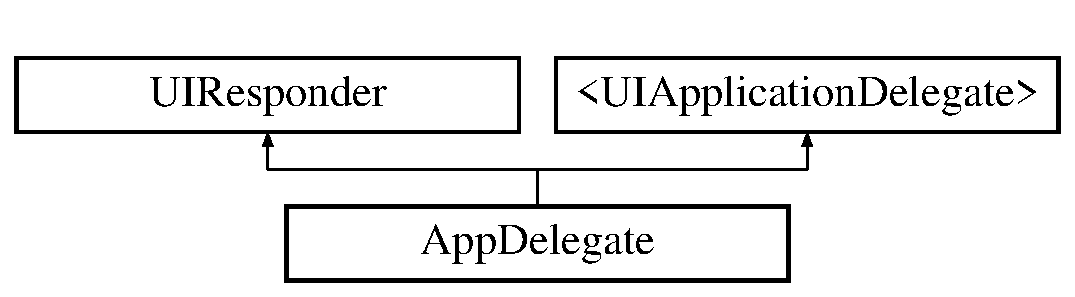
\includegraphics[height=2.000000cm]{interface_app_delegate}
\end{center}
\end{figure}
\subsection*{Instance Methods}
\begin{DoxyCompactItemize}
\item 
(B\-O\-O\-L) -\/ \hyperlink{interface_app_delegate_a8cf55cdca24f5077db73eab11a17dedf}{application\-:open\-U\-R\-L\-:source\-Application\-:annotation\-:}
\item 
\hypertarget{interface_app_delegate_a2fe81b234fcf8951be6ebc785d4f1a42}{(void) -\/ \hyperlink{interface_app_delegate_a2fe81b234fcf8951be6ebc785d4f1a42}{detect\-Orientation}}\label{interface_app_delegate_a2fe81b234fcf8951be6ebc785d4f1a42}

\begin{DoxyCompactList}\small\item\em Notifies the logger that the user is rotating the i\-Pad. \end{DoxyCompactList}\end{DoxyCompactItemize}
\subsection*{Properties}
\begin{DoxyCompactItemize}
\item 
\hypertarget{interface_app_delegate_a26c59ea8851d81cef0871b61ce2e1b43}{\hyperlink{interface_m_f_side_menu_container_view_controller}{M\-F\-Side\-Menu\-Container\-View\-Controller} $\ast$ \hyperlink{interface_app_delegate_a26c59ea8851d81cef0871b61ce2e1b43}{container}}\label{interface_app_delegate_a26c59ea8851d81cef0871b61ce2e1b43}

\begin{DoxyCompactList}\small\item\em A pointer to our canvas to create models. \end{DoxyCompactList}\item 
\hypertarget{interface_app_delegate_ae04748cdefebda525b266731b6c120a2}{U\-I\-Window $\ast$ \hyperlink{interface_app_delegate_ae04748cdefebda525b266731b6c120a2}{window}}\label{interface_app_delegate_ae04748cdefebda525b266731b6c120a2}

\begin{DoxyCompactList}\small\item\em The window of the application. \end{DoxyCompactList}\end{DoxyCompactItemize}


\subsection{Detailed Description}
The U\-I\-Responder class defines an interface for objects that respond to and handle events. It is the superclass of U\-I\-Application, U\-I\-View and its subclasses (which include U\-I\-Window). Instances of these classes are sometimes referred to as responder objects or, simply, responders. 

\subsection{Method Documentation}
\hypertarget{interface_app_delegate_a8cf55cdca24f5077db73eab11a17dedf}{\index{App\-Delegate@{App\-Delegate}!application\-:open\-U\-R\-L\-:source\-Application\-:annotation\-:@{application\-:open\-U\-R\-L\-:source\-Application\-:annotation\-:}}
\index{application\-:open\-U\-R\-L\-:source\-Application\-:annotation\-:@{application\-:open\-U\-R\-L\-:source\-Application\-:annotation\-:}!AppDelegate@{App\-Delegate}}
\subsubsection[{application\-:open\-U\-R\-L\-:source\-Application\-:annotation\-:}]{\setlength{\rightskip}{0pt plus 5cm}-\/ (B\-O\-O\-L) application\-: 
\begin{DoxyParamCaption}
\item[{(U\-I\-Application $\ast$)}]{app}
\item[{openURL:(N\-S\-U\-R\-L $\ast$)}]{url}
\item[{sourceApplication:(N\-S\-String $\ast$)}]{source}
\item[{annotation:(id)}]{annotation}
\end{DoxyParamCaption}
}}\label{interface_app_delegate_a8cf55cdca24f5077db73eab11a17dedf}
Method used to handle the linkage between my app and Dropbox. 
\begin{DoxyParams}{Parameters}
{\em app} & the application making the call. \\
\hline
{\em url} & the url of the file we would like to choose. \\
\hline
{\em source} & the source application. \\
\hline
{\em annotation} & \\
\hline
\end{DoxyParams}
\begin{DoxyReturn}{Returns}
a boolean value if whether or not the url can be opened. 
\end{DoxyReturn}


The documentation for this class was generated from the following files\-:\begin{DoxyCompactItemize}
\item 
Group\-Modeling\-App/App\-Delegate.\-h\item 
Group\-Modeling\-App/App\-Delegate.\-m\end{DoxyCompactItemize}

\hypertarget{interface_causal_link}{\section{Causal\-Link Class Reference}
\label{interface_causal_link}\index{Causal\-Link@{Causal\-Link}}
}


A subclass of \hyperlink{interface_component}{Component} containing the data related to a causal link between two variables of a causal loop diagram. ex. In a diagram on Childhood obesity, there may exist a relationship between the \char`\"{}\-Fast Food Consumption\char`\"{} variable and the \char`\"{}\-Weight Gain\char`\"{} variable. This class represents that causal link.  




{\ttfamily \#import $<$Causal\-Link.\-h$>$}

Inheritance diagram for Causal\-Link\-:\begin{figure}[H]
\begin{center}
\leavevmode
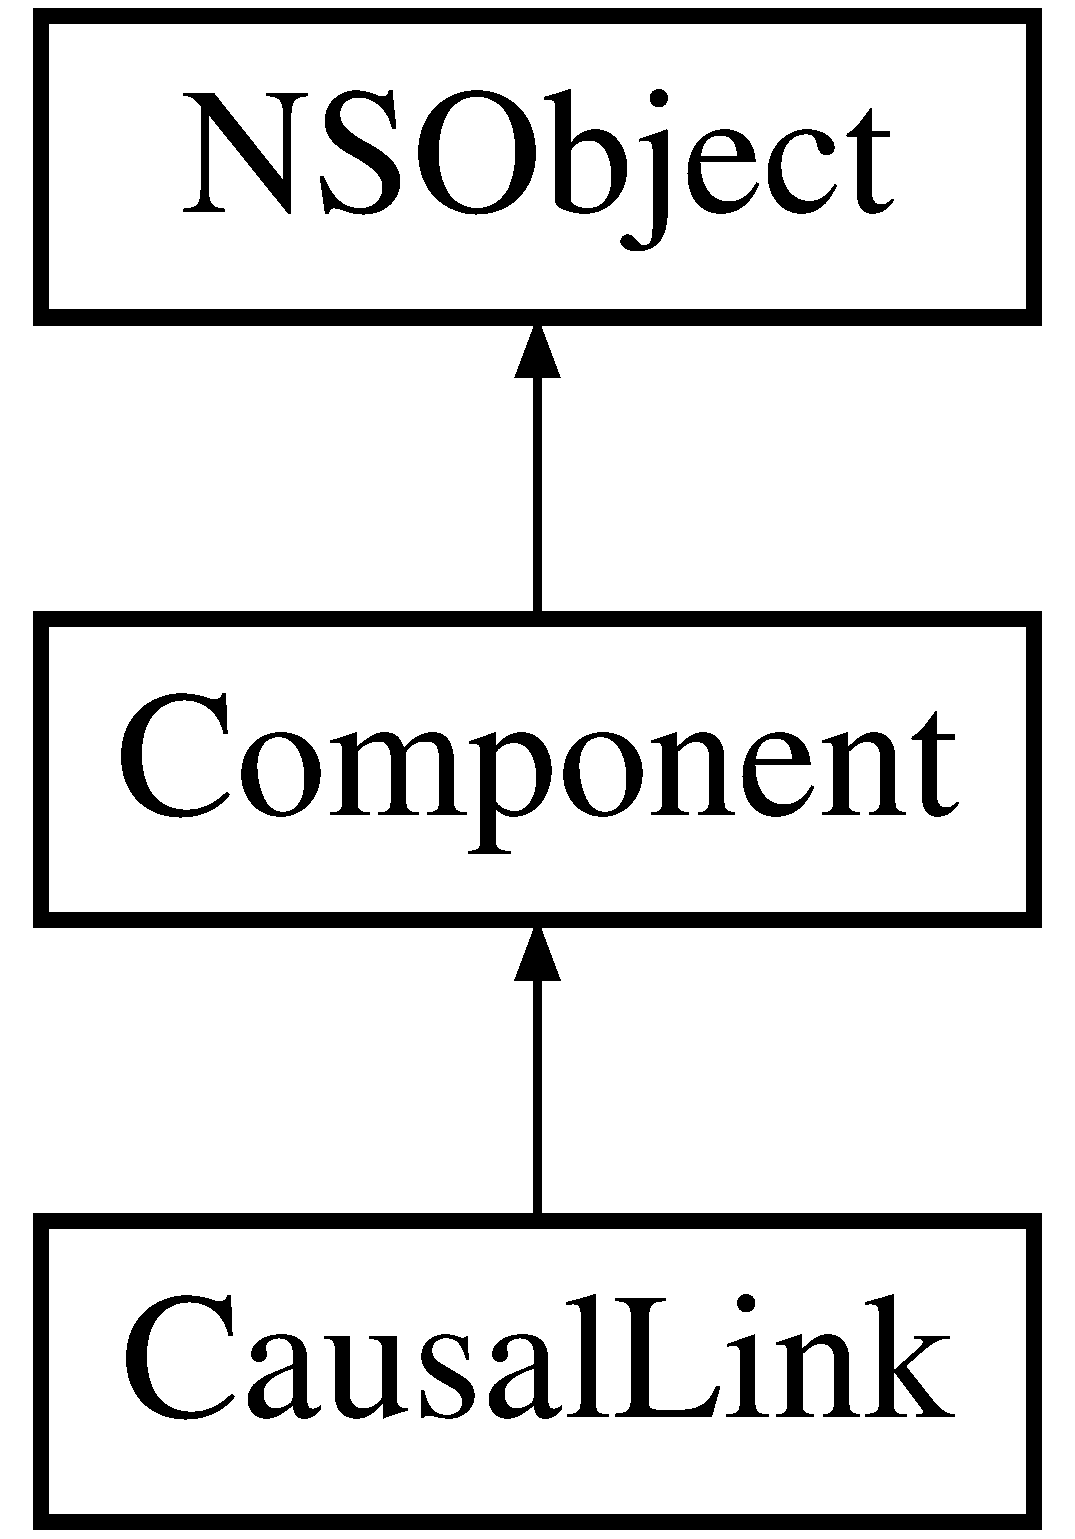
\includegraphics[height=3.000000cm]{interface_causal_link}
\end{center}
\end{figure}
\subsection*{Instance Methods}
\begin{DoxyCompactItemize}
\item 
(id) -\/ \hyperlink{interface_causal_link_ae3fdc3a923d3d3be4b4aeb821cb90734}{init\-:}
\item 
(id) -\/ \hyperlink{interface_causal_link_a80971dff11e8048c269097f9e94279fc}{init\-With\-Parent\-:and\-Child\-:}
\item 
(void) -\/ \hyperlink{interface_causal_link_ae6b612c2817771b1fd4d12b1b0ac56d3}{create\-View}
\item 
(N\-S\-String $\ast$) -\/ \hyperlink{interface_causal_link_aeaeca5d45f4b917997bfea36c86dc4b1}{create\-Causal\-Link\-Output\-String}
\item 
(U\-I\-Color $\ast$) -\/ \hyperlink{interface_causal_link_a81afff0a3a22627c88301943c5228a6a}{convert\-To\-U\-I\-Color\-:and\-Green\-:and\-Blue\-:}
\item 
(N\-S\-String $\ast$) -\/ \hyperlink{interface_causal_link_acdb5a57ca0f4f77aee198dff20a2ea57}{convert\-From\-U\-I\-Color\-:}
\end{DoxyCompactItemize}
\subsection*{Class Methods}
\begin{DoxyCompactItemize}
\item 
(N\-S\-String $\ast$) + \hyperlink{interface_causal_link_a58132842dd002d42efcdef8bd0d7ee79}{get\-Color\-Name\-:}
\end{DoxyCompactItemize}
\subsection*{Properties}
\begin{DoxyCompactItemize}
\item 
\hypertarget{interface_causal_link_a92793d006bbec1b2ac27bb8f580fe2af}{id \hyperlink{interface_causal_link_a92793d006bbec1b2ac27bb8f580fe2af}{parent\-Object}}\label{interface_causal_link_a92793d006bbec1b2ac27bb8f580fe2af}

\begin{DoxyCompactList}\small\item\em A pointer to the source variable of the causal link. \end{DoxyCompactList}\item 
\hypertarget{interface_causal_link_a89bb83f507d8a9c64e76958adfe99676}{id \hyperlink{interface_causal_link_a89bb83f507d8a9c64e76958adfe99676}{child\-Object}}\label{interface_causal_link_a89bb83f507d8a9c64e76958adfe99676}

\begin{DoxyCompactList}\small\item\em A pointer to the influenced variable of the causal link. \end{DoxyCompactList}\item 
\hypertarget{interface_causal_link_a698e70e52e27741aee1a7e5bfe44c468}{\hyperlink{interface_causal_link_view}{Causal\-Link\-View} $\ast$ \hyperlink{interface_causal_link_a698e70e52e27741aee1a7e5bfe44c468}{view}}\label{interface_causal_link_a698e70e52e27741aee1a7e5bfe44c468}

\begin{DoxyCompactList}\small\item\em The U\-I\-View that will contain the graphical representation of the causal link. \end{DoxyCompactList}\end{DoxyCompactItemize}


\subsection{Detailed Description}
A subclass of \hyperlink{interface_component}{Component} containing the data related to a causal link between two variables of a causal loop diagram. ex. In a diagram on Childhood obesity, there may exist a relationship between the \char`\"{}\-Fast Food Consumption\char`\"{} variable and the \char`\"{}\-Weight Gain\char`\"{} variable. This class represents that causal link. 

\subsection{Method Documentation}
\hypertarget{interface_causal_link_acdb5a57ca0f4f77aee198dff20a2ea57}{\index{Causal\-Link@{Causal\-Link}!convert\-From\-U\-I\-Color\-:@{convert\-From\-U\-I\-Color\-:}}
\index{convert\-From\-U\-I\-Color\-:@{convert\-From\-U\-I\-Color\-:}!CausalLink@{Causal\-Link}}
\subsubsection[{convert\-From\-U\-I\-Color\-:}]{\setlength{\rightskip}{0pt plus 5cm}-\/ (N\-S\-String $\ast$) convert\-From\-U\-I\-Color\-: 
\begin{DoxyParamCaption}
\item[{(U\-I\-Color$\ast$)}]{color}
\end{DoxyParamCaption}
}}\label{interface_causal_link_acdb5a57ca0f4f77aee198dff20a2ea57}
Converts a U\-I\-Color to its R\-G\-B equivalent. 
\begin{DoxyParams}{Parameters}
{\em color} & the U\-I\-Color you want to get the corresponding R\-G\-B value for. \\
\hline
\end{DoxyParams}
\begin{DoxyReturn}{Returns}
an rgb string value for color ,R-\/\-G-\/\-B. 
\end{DoxyReturn}
\hypertarget{interface_causal_link_a81afff0a3a22627c88301943c5228a6a}{\index{Causal\-Link@{Causal\-Link}!convert\-To\-U\-I\-Color\-:and\-Green\-:and\-Blue\-:@{convert\-To\-U\-I\-Color\-:and\-Green\-:and\-Blue\-:}}
\index{convert\-To\-U\-I\-Color\-:and\-Green\-:and\-Blue\-:@{convert\-To\-U\-I\-Color\-:and\-Green\-:and\-Blue\-:}!CausalLink@{Causal\-Link}}
\subsubsection[{convert\-To\-U\-I\-Color\-:and\-Green\-:and\-Blue\-:}]{\setlength{\rightskip}{0pt plus 5cm}-\/ (U\-I\-Color $\ast$) convert\-To\-U\-I\-Color\-: 
\begin{DoxyParamCaption}
\item[{(int)}]{red}
\item[{andGreen:(int)}]{green}
\item[{andBlue:(int)}]{blue}
\end{DoxyParamCaption}
}}\label{interface_causal_link_a81afff0a3a22627c88301943c5228a6a}
Converts an R\-G\-B value to a U\-I\-Color. The R\-G\-B values used in the code are the R\-G\-B equivalent of colors used in Vensim. 
\begin{DoxyParams}{Parameters}
{\em red} & the red value from 0-\/255. \\
\hline
{\em green} & the green value from 0-\/255. \\
\hline
{\em blue} & the blue value from 0-\/255. \\
\hline
\end{DoxyParams}
\begin{DoxyReturn}{Returns}
the U\-I\-Color associated with the R\-G\-B values passed in, black if a match not found. 
\end{DoxyReturn}
\hypertarget{interface_causal_link_aeaeca5d45f4b917997bfea36c86dc4b1}{\index{Causal\-Link@{Causal\-Link}!create\-Causal\-Link\-Output\-String@{create\-Causal\-Link\-Output\-String}}
\index{create\-Causal\-Link\-Output\-String@{create\-Causal\-Link\-Output\-String}!CausalLink@{Causal\-Link}}
\subsubsection[{create\-Causal\-Link\-Output\-String}]{\setlength{\rightskip}{0pt plus 5cm}-\/ (N\-S\-String $\ast$) create\-Causal\-Link\-Output\-String 
\begin{DoxyParamCaption}
{}
\end{DoxyParamCaption}
}}\label{interface_causal_link_aeaeca5d45f4b917997bfea36c86dc4b1}
Constructs the output string for a \hyperlink{interface_causal_link}{Causal\-Link}. The string is constructed to be readable by Vensim. Follows the string pattern\-: \mbox{[}Object Type\mbox{]},\mbox{[}Object id\mbox{]}, \mbox{[}Starting Object id\mbox{]},\mbox{[}Ending Object id\mbox{]},1,0,\mbox{[}Polarity\mbox{]},\mbox{[}Line thickness\mbox{]},3,\mbox{[}Delay/\-Polarity Position\mbox{]},0,\mbox{[}Arrow Color\mbox{]},\mbox{[}Font Size\mbox{]},\mbox{[}Font Color\mbox{]},\mbox{[}Handle Position\mbox{]} \begin{DoxyReturn}{Returns}
the Vensim string of data for the \hyperlink{interface_causal_link}{Causal\-Link}. 
\end{DoxyReturn}
\hypertarget{interface_causal_link_ae6b612c2817771b1fd4d12b1b0ac56d3}{\index{Causal\-Link@{Causal\-Link}!create\-View@{create\-View}}
\index{create\-View@{create\-View}!CausalLink@{Causal\-Link}}
\subsubsection[{create\-View}]{\setlength{\rightskip}{0pt plus 5cm}-\/ (void) create\-View 
\begin{DoxyParamCaption}
{}
\end{DoxyParamCaption}
}}\label{interface_causal_link_ae6b612c2817771b1fd4d12b1b0ac56d3}
When initially importing the file, a \hyperlink{interface_causal_link}{Causal\-Link} does not know the location of its parent and child, but knows the id of the parent and child. Once the file has been parsed through completely, \hyperlink{interface_file_i_o}{File\-I\-O} will revisit the Causal\-Links and set the parent\-Object and the child\-Object to the corresponding \hyperlink{interface_variable}{Variable} instances. This method updates the start\-Point, end\-Point, control\-Point located in the view based on the updated parent and child objects. After the points of the arc have been set, the frame of the view will be calculated and the view will be added to the parentview. 
\begin{DoxyParams}{Parameters}
{\em parent\-View} & the superview that the \hyperlink{interface_causal_link}{Causal\-Link} view will be added as a subview. \\
\hline
\end{DoxyParams}
\hypertarget{interface_causal_link_a58132842dd002d42efcdef8bd0d7ee79}{\index{Causal\-Link@{Causal\-Link}!get\-Color\-Name\-:@{get\-Color\-Name\-:}}
\index{get\-Color\-Name\-:@{get\-Color\-Name\-:}!CausalLink@{Causal\-Link}}
\subsubsection[{get\-Color\-Name\-:}]{\setlength{\rightskip}{0pt plus 5cm}+ (N\-S\-String $\ast$) get\-Color\-Name\-: 
\begin{DoxyParamCaption}
\item[{(U\-I\-Color$\ast$)}]{color}
\end{DoxyParamCaption}
}}\label{interface_causal_link_a58132842dd002d42efcdef8bd0d7ee79}
Gets the textual representation of a color. 
\begin{DoxyParams}{Parameters}
{\em color} & the uicolor that you want to get the name of. \\
\hline
\end{DoxyParams}
\begin{DoxyReturn}{Returns}
the name of the color as a string. 
\end{DoxyReturn}
\hypertarget{interface_causal_link_ae3fdc3a923d3d3be4b4aeb821cb90734}{\index{Causal\-Link@{Causal\-Link}!init\-:@{init\-:}}
\index{init\-:@{init\-:}!CausalLink@{Causal\-Link}}
\subsubsection[{init\-:}]{\setlength{\rightskip}{0pt plus 5cm}-\/ (id) init\-: 
\begin{DoxyParamCaption}
\item[{(N\-S\-Array$\ast$)}]{data}
\end{DoxyParamCaption}
}}\label{interface_causal_link_ae3fdc3a923d3d3be4b4aeb821cb90734}
Initializes the \hyperlink{interface_causal_link}{Causal\-Link}. 
\begin{DoxyParams}{Parameters}
{\em data} & an array of strings containing all of the data for the causal link from a Vensim mdl file. \\
\hline
\end{DoxyParams}
\begin{DoxyReturn}{Returns}
a pointer to the newly created causal link. 
\end{DoxyReturn}
The parent and child objects will point to integers initially. Once the entire model is parsed, the \hyperlink{interface_file_i_o}{File\-I\-O} class will update these objects to point to the associated variable objects. \hypertarget{interface_causal_link_a80971dff11e8048c269097f9e94279fc}{\index{Causal\-Link@{Causal\-Link}!init\-With\-Parent\-:and\-Child\-:@{init\-With\-Parent\-:and\-Child\-:}}
\index{init\-With\-Parent\-:and\-Child\-:@{init\-With\-Parent\-:and\-Child\-:}!CausalLink@{Causal\-Link}}
\subsubsection[{init\-With\-Parent\-:and\-Child\-:}]{\setlength{\rightskip}{0pt plus 5cm}-\/ (id) init\-With\-Parent\-: 
\begin{DoxyParamCaption}
\item[{({\bf Variable}$\ast$)}]{parent}
\item[{andChild:({\bf Variable}$\ast$)}]{child}
\end{DoxyParamCaption}
}}\label{interface_causal_link_a80971dff11e8048c269097f9e94279fc}
Initializes the \hyperlink{interface_causal_link}{Causal\-Link}. 
\begin{DoxyParams}{Parameters}
{\em parent} & the parent variable object that the causal link begins from. \\
\hline
{\em child} & the child object that the causal link points to. \\
\hline
\end{DoxyParams}
\begin{DoxyReturn}{Returns}
a pointer to the newly created causal link. 
\end{DoxyReturn}


The documentation for this class was generated from the following files\-:\begin{DoxyCompactItemize}
\item 
Group\-Modeling\-App/Causal\-Link.\-h\item 
Group\-Modeling\-App/Causal\-Link.\-m\end{DoxyCompactItemize}

\hypertarget{interface_causal_link_edit_menu_view}{\section{Causal\-Link\-Edit\-Menu\-View Class Reference}
\label{interface_causal_link_edit_menu_view}\index{Causal\-Link\-Edit\-Menu\-View@{Causal\-Link\-Edit\-Menu\-View}}
}


The view that will contain the edit menu for Causal\-Links.  




{\ttfamily \#import $<$Causal\-Link\-Edit\-Menu\-View.\-h$>$}

Inheritance diagram for Causal\-Link\-Edit\-Menu\-View\-:\begin{figure}[H]
\begin{center}
\leavevmode
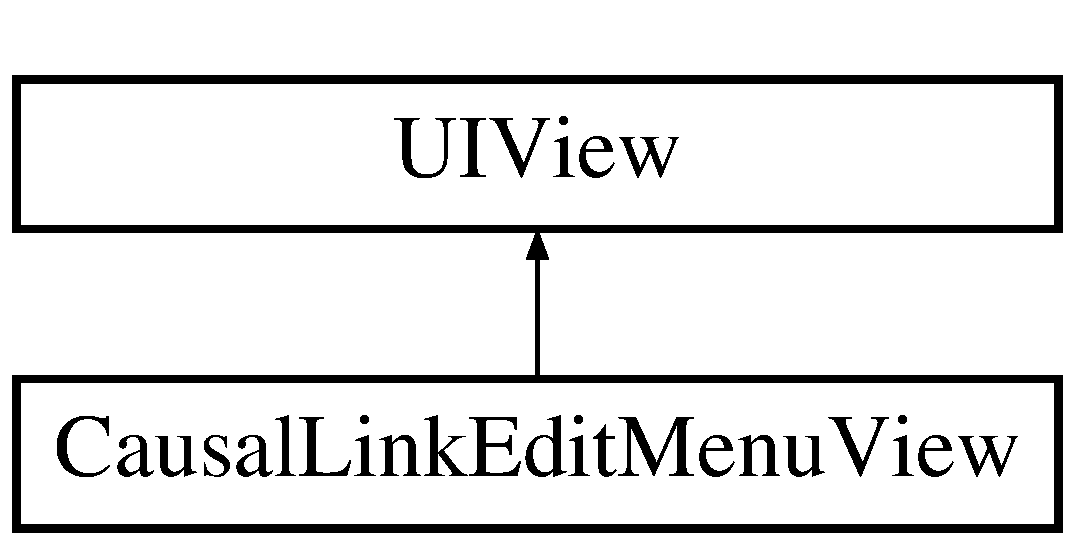
\includegraphics[height=2.000000cm]{interface_causal_link_edit_menu_view}
\end{center}
\end{figure}
\subsection*{Instance Methods}
\begin{DoxyCompactItemize}
\item 
(id) -\/ \hyperlink{interface_causal_link_edit_menu_view_ad1475d40e606d4f009f89321944e3678}{init\-With\-Frame\-:view\-:}
\item 
\hypertarget{interface_causal_link_edit_menu_view_ae23c342ee9fb7ce665b7354c3fb4b222}{(void) -\/ \hyperlink{interface_causal_link_edit_menu_view_ae23c342ee9fb7ce665b7354c3fb4b222}{update\-Causal\-Link}}\label{interface_causal_link_edit_menu_view_ae23c342ee9fb7ce665b7354c3fb4b222}

\begin{DoxyCompactList}\small\item\em This method will be called when the save button is called to save the attributes. \end{DoxyCompactList}\item 
(U\-I\-Color $\ast$) -\/ \hyperlink{interface_causal_link_edit_menu_view_ae738ae72f04ce87c6338636677f00d29}{get\-Color}
\item 
(int) -\/ \hyperlink{interface_causal_link_edit_menu_view_a6dbd080e76ce4ee3d6977c62f72e49b4}{get\-Color\-Index}
\item 
\hypertarget{interface_causal_link_edit_menu_view_aa58a2d9c88390d1274785ab09ac523f0}{(void) -\/ \hyperlink{interface_causal_link_edit_menu_view_aa58a2d9c88390d1274785ab09ac523f0}{polarity\-Controls\-Change}}\label{interface_causal_link_edit_menu_view_aa58a2d9c88390d1274785ab09ac523f0}

\begin{DoxyCompactList}\small\item\em Notifies the logger when a new option from the polarity segmented control has been changed. \end{DoxyCompactList}\item 
\hypertarget{interface_causal_link_edit_menu_view_ab36ea37c4278dd582eecb569ec96cd4e}{(void) -\/ \hyperlink{interface_causal_link_edit_menu_view_ab36ea37c4278dd582eecb569ec96cd4e}{line\-Thickness\-Controls\-Change}}\label{interface_causal_link_edit_menu_view_ab36ea37c4278dd582eecb569ec96cd4e}

\begin{DoxyCompactList}\small\item\em Notifies the logger when a new option from the line thickness segmented control has been changed. \end{DoxyCompactList}\item 
\hypertarget{interface_causal_link_edit_menu_view_a1205630474a5a56a221ede7c02b97d16}{(void) -\/ \hyperlink{interface_causal_link_edit_menu_view_a1205630474a5a56a221ede7c02b97d16}{time\-Delay\-Controls\-Change}}\label{interface_causal_link_edit_menu_view_a1205630474a5a56a221ede7c02b97d16}

\begin{DoxyCompactList}\small\item\em Notifies the logger when a new option from the time delay segmented control has been changed. \end{DoxyCompactList}\item 
\hypertarget{interface_causal_link_edit_menu_view_ab6f1c074117b868e4fb13c929b97643a}{(void) -\/ \hyperlink{interface_causal_link_edit_menu_view_ab6f1c074117b868e4fb13c929b97643a}{color\-Picker\-Controls\-Change}}\label{interface_causal_link_edit_menu_view_ab6f1c074117b868e4fb13c929b97643a}

\begin{DoxyCompactList}\small\item\em Notifies the logger when a new option from the color picker segmented control has been changed. \end{DoxyCompactList}\end{DoxyCompactItemize}
\subsection*{Properties}
\begin{DoxyCompactItemize}
\item 
\hypertarget{interface_causal_link_edit_menu_view_abf252978f516cd3031621f8b4dbc55a1}{U\-I\-Segmented\-Control $\ast$ \hyperlink{interface_causal_link_edit_menu_view_abf252978f516cd3031621f8b4dbc55a1}{line\-Thickness\-Controls}}\label{interface_causal_link_edit_menu_view_abf252978f516cd3031621f8b4dbc55a1}

\begin{DoxyCompactList}\small\item\em The segmented control that allows the user to change the line thickness. \end{DoxyCompactList}\item 
\hypertarget{interface_causal_link_edit_menu_view_a435537f3bc8e923f4eb7d1d943f9eadc}{U\-I\-Label $\ast$ \hyperlink{interface_causal_link_edit_menu_view_a435537f3bc8e923f4eb7d1d943f9eadc}{line\-Thickness\-Label}}\label{interface_causal_link_edit_menu_view_a435537f3bc8e923f4eb7d1d943f9eadc}

\begin{DoxyCompactList}\small\item\em The label that represents what line\-Thickness\-Controls represents. \end{DoxyCompactList}\item 
\hypertarget{interface_causal_link_edit_menu_view_a930d57d36d2318aaf652f8914afd17bf}{\hyperlink{interface_causal_link_view}{Causal\-Link\-View} $\ast$ \hyperlink{interface_causal_link_edit_menu_view_a930d57d36d2318aaf652f8914afd17bf}{object\-View}}\label{interface_causal_link_edit_menu_view_a930d57d36d2318aaf652f8914afd17bf}

\begin{DoxyCompactList}\small\item\em The view of the object that you are editing. \end{DoxyCompactList}\item 
\hypertarget{interface_causal_link_edit_menu_view_a084f50dc82d79d565c48f15bb3b7746d}{U\-I\-Segmented\-Control $\ast$ \hyperlink{interface_causal_link_edit_menu_view_a084f50dc82d79d565c48f15bb3b7746d}{polarity\-Controls}}\label{interface_causal_link_edit_menu_view_a084f50dc82d79d565c48f15bb3b7746d}

\begin{DoxyCompactList}\small\item\em The segmented control that allows the user to change the polarity. \end{DoxyCompactList}\item 
\hypertarget{interface_causal_link_edit_menu_view_adf6a823fbc18324bccd978afe58a26b1}{U\-I\-Label $\ast$ \hyperlink{interface_causal_link_edit_menu_view_adf6a823fbc18324bccd978afe58a26b1}{polarity\-Label}}\label{interface_causal_link_edit_menu_view_adf6a823fbc18324bccd978afe58a26b1}

\begin{DoxyCompactList}\small\item\em The label that represents what polarity\-Controls represents. \end{DoxyCompactList}\item 
\hypertarget{interface_causal_link_edit_menu_view_ac946d255eefec0ce4de0fa405900e209}{U\-I\-Segmented\-Control $\ast$ \hyperlink{interface_causal_link_edit_menu_view_ac946d255eefec0ce4de0fa405900e209}{time\-Delay\-Controls}}\label{interface_causal_link_edit_menu_view_ac946d255eefec0ce4de0fa405900e209}

\begin{DoxyCompactList}\small\item\em The segmented control that allows the user to turn on the time delay. \end{DoxyCompactList}\item 
\hypertarget{interface_causal_link_edit_menu_view_a14a3cab7d4f306f368b8707350970405}{U\-I\-Label $\ast$ \hyperlink{interface_causal_link_edit_menu_view_a14a3cab7d4f306f368b8707350970405}{time\-Delay\-Label}}\label{interface_causal_link_edit_menu_view_a14a3cab7d4f306f368b8707350970405}

\begin{DoxyCompactList}\small\item\em The label that represents what time\-Delay\-Controls represents. \end{DoxyCompactList}\item 
\hypertarget{interface_causal_link_edit_menu_view_a7e936d3c7aed4d5661f4f3e39b62c3b9}{U\-I\-Label $\ast$ \hyperlink{interface_causal_link_edit_menu_view_a7e936d3c7aed4d5661f4f3e39b62c3b9}{color\-Picker\-Label}}\label{interface_causal_link_edit_menu_view_a7e936d3c7aed4d5661f4f3e39b62c3b9}

\begin{DoxyCompactList}\small\item\em The label that represents what color\-Picker represents. \end{DoxyCompactList}\item 
\hypertarget{interface_causal_link_edit_menu_view_ac51c7f33f6b3c383f52b0b5958a7d05e}{U\-I\-Segmented\-Control $\ast$ \hyperlink{interface_causal_link_edit_menu_view_ac51c7f33f6b3c383f52b0b5958a7d05e}{color\-Picker}}\label{interface_causal_link_edit_menu_view_ac51c7f33f6b3c383f52b0b5958a7d05e}

\begin{DoxyCompactList}\small\item\em The segmented control that allows the user to change the polarity. \end{DoxyCompactList}\end{DoxyCompactItemize}


\subsection{Detailed Description}
The view that will contain the edit menu for Causal\-Links. 

\subsection{Method Documentation}
\hypertarget{interface_causal_link_edit_menu_view_ae738ae72f04ce87c6338636677f00d29}{\index{Causal\-Link\-Edit\-Menu\-View@{Causal\-Link\-Edit\-Menu\-View}!get\-Color@{get\-Color}}
\index{get\-Color@{get\-Color}!CausalLinkEditMenuView@{Causal\-Link\-Edit\-Menu\-View}}
\subsubsection[{get\-Color}]{\setlength{\rightskip}{0pt plus 5cm}-\/ (U\-I\-Color $\ast$) get\-Color 
\begin{DoxyParamCaption}
{}
\end{DoxyParamCaption}
}}\label{interface_causal_link_edit_menu_view_ae738ae72f04ce87c6338636677f00d29}
Gets the corresponding U\-I\-Color related to the selected segment index. \begin{DoxyReturn}{Returns}
an instance of a U\-I\-Color used to set the color of the arc. 
\end{DoxyReturn}
\hypertarget{interface_causal_link_edit_menu_view_a6dbd080e76ce4ee3d6977c62f72e49b4}{\index{Causal\-Link\-Edit\-Menu\-View@{Causal\-Link\-Edit\-Menu\-View}!get\-Color\-Index@{get\-Color\-Index}}
\index{get\-Color\-Index@{get\-Color\-Index}!CausalLinkEditMenuView@{Causal\-Link\-Edit\-Menu\-View}}
\subsubsection[{get\-Color\-Index}]{\setlength{\rightskip}{0pt plus 5cm}-\/ (int) get\-Color\-Index 
\begin{DoxyParamCaption}
{}
\end{DoxyParamCaption}
}}\label{interface_causal_link_edit_menu_view_a6dbd080e76ce4ee3d6977c62f72e49b4}
Get the segement index based on the current color of the causal link. \begin{DoxyReturn}{Returns}
an integer representing a index of the segmented control. 
\end{DoxyReturn}
\hypertarget{interface_causal_link_edit_menu_view_ad1475d40e606d4f009f89321944e3678}{\index{Causal\-Link\-Edit\-Menu\-View@{Causal\-Link\-Edit\-Menu\-View}!init\-With\-Frame\-:view\-:@{init\-With\-Frame\-:view\-:}}
\index{init\-With\-Frame\-:view\-:@{init\-With\-Frame\-:view\-:}!CausalLinkEditMenuView@{Causal\-Link\-Edit\-Menu\-View}}
\subsubsection[{init\-With\-Frame\-:view\-:}]{\setlength{\rightskip}{0pt plus 5cm}-\/ (id) init\-With\-Frame\-: 
\begin{DoxyParamCaption}
\item[{(C\-G\-Rect)}]{frame}
\item[{view:(U\-I\-View$\ast$)}]{view}
\end{DoxyParamCaption}
}}\label{interface_causal_link_edit_menu_view_ad1475d40e606d4f009f89321944e3678}
Initializes the view. 
\begin{DoxyParams}{Parameters}
{\em frame} & the frame the view is contained within. \\
\hline
{\em view} & the uiview of the object that the menu is being created for. \\
\hline
\end{DoxyParams}
\begin{DoxyReturn}{Returns}
an id of the newly created view. 
\end{DoxyReturn}


The documentation for this class was generated from the following files\-:\begin{DoxyCompactItemize}
\item 
Group\-Modeling\-App/Causal\-Link\-Edit\-Menu\-View.\-h\item 
Group\-Modeling\-App/Causal\-Link\-Edit\-Menu\-View.\-m\end{DoxyCompactItemize}

\hypertarget{interface_causal_link_handle_view}{\section{Causal\-Link\-Handle\-View Class Reference}
\label{interface_causal_link_handle_view}\index{Causal\-Link\-Handle\-View@{Causal\-Link\-Handle\-View}}
}


A view that display the vertex of the \hyperlink{interface_causal_link}{Causal\-Link}. This view is also used to move and modify the \hyperlink{interface_causal_link}{Causal\-Link}.  




{\ttfamily \#import $<$Causal\-Link\-Handle\-View.\-h$>$}

Inheritance diagram for Causal\-Link\-Handle\-View\-:\begin{figure}[H]
\begin{center}
\leavevmode
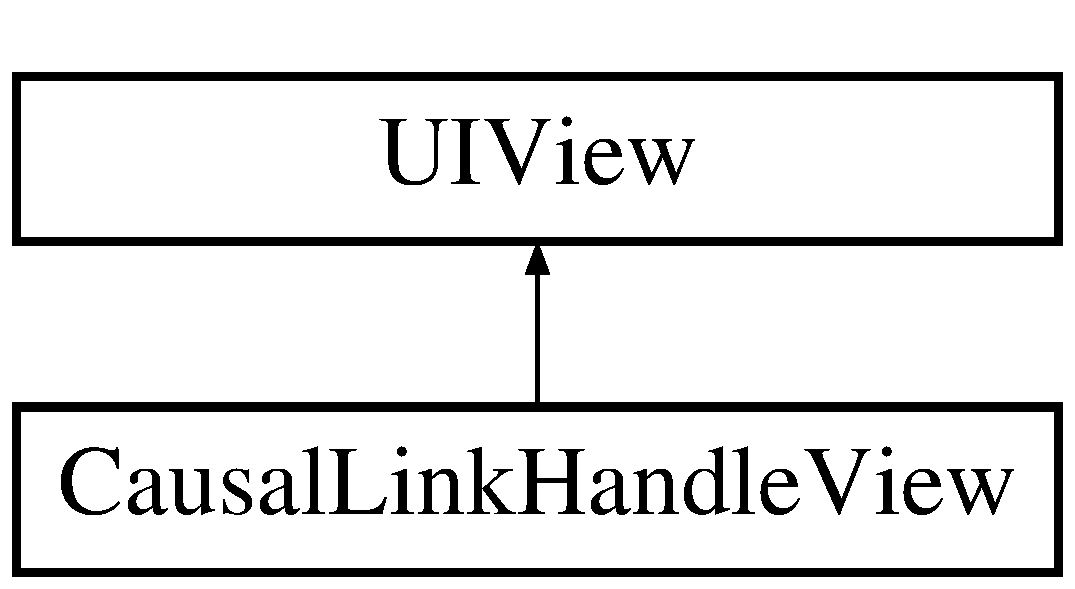
\includegraphics[height=2.000000cm]{interface_causal_link_handle_view}
\end{center}
\end{figure}
\subsection*{Instance Methods}
\begin{DoxyCompactItemize}
\item 
(id) -\/ \hyperlink{interface_causal_link_handle_view_a100c2da2d92d7d9a4da9ad851dcc1114}{init\-With\-Frame\-:}
\item 
(void) -\/ \hyperlink{interface_causal_link_handle_view_a8c03538769a6fcbd7aa8e672cf4b5c96}{draw\-Rect\-:}
\item 
(void) -\/ \hyperlink{interface_causal_link_handle_view_a2357112d7fefe9f720ac82c881236830}{touches\-Began\-:with\-Event\-:}
\item 
(void) -\/ \hyperlink{interface_causal_link_handle_view_a06bf1152e9fa0dd16bf7f46128ae0cff}{touches\-Moved\-:with\-Event\-:}
\item 
(void) -\/ \hyperlink{interface_causal_link_handle_view_ad9cc995e0aa0c5e28ab827a06c897c36}{touches\-Ended\-:with\-Event\-:}
\item 
(void) -\/ \hyperlink{interface_causal_link_handle_view_a38393b10eebe5376725616eb446df377}{handle\-Single\-Tap\-:}
\end{DoxyCompactItemize}
\subsection*{Properties}
\begin{DoxyCompactItemize}
\item 
\hypertarget{interface_causal_link_handle_view_a5575d6f2d41b9179b560b7f3857ca1db}{\hyperlink{interface_causal_link_view}{Causal\-Link\-View} $\ast$ \hyperlink{interface_causal_link_handle_view_a5575d6f2d41b9179b560b7f3857ca1db}{parent}}\label{interface_causal_link_handle_view_a5575d6f2d41b9179b560b7f3857ca1db}

\begin{DoxyCompactList}\small\item\em A pointer to the parent \hyperlink{interface_causal_link_view}{Causal\-Link\-View} that the handle is attached to. \end{DoxyCompactList}\end{DoxyCompactItemize}


\subsection{Detailed Description}
A view that display the vertex of the \hyperlink{interface_causal_link}{Causal\-Link}. This view is also used to move and modify the \hyperlink{interface_causal_link}{Causal\-Link}. 

\subsection{Method Documentation}
\hypertarget{interface_causal_link_handle_view_a8c03538769a6fcbd7aa8e672cf4b5c96}{\index{Causal\-Link\-Handle\-View@{Causal\-Link\-Handle\-View}!draw\-Rect\-:@{draw\-Rect\-:}}
\index{draw\-Rect\-:@{draw\-Rect\-:}!CausalLinkHandleView@{Causal\-Link\-Handle\-View}}
\subsubsection[{draw\-Rect\-:}]{\setlength{\rightskip}{0pt plus 5cm}-\/ (void) draw\-Rect\-: 
\begin{DoxyParamCaption}
\item[{(C\-G\-Rect)}]{rect}
\end{DoxyParamCaption}
}}\label{interface_causal_link_handle_view_a8c03538769a6fcbd7aa8e672cf4b5c96}
Draws the receiver’s image within the passed-\/in rectangle. This is an overridden method. 
\begin{DoxyParams}{Parameters}
{\em rect} & the frame of the view in which objects can be drawn. \\
\hline
\end{DoxyParams}
\hypertarget{interface_causal_link_handle_view_a38393b10eebe5376725616eb446df377}{\index{Causal\-Link\-Handle\-View@{Causal\-Link\-Handle\-View}!handle\-Single\-Tap\-:@{handle\-Single\-Tap\-:}}
\index{handle\-Single\-Tap\-:@{handle\-Single\-Tap\-:}!CausalLinkHandleView@{Causal\-Link\-Handle\-View}}
\subsubsection[{handle\-Single\-Tap\-:}]{\setlength{\rightskip}{0pt plus 5cm}-\/ (void) handle\-Single\-Tap\-: 
\begin{DoxyParamCaption}
\item[{(U\-I\-Tap\-Gesture\-Recognizer $\ast$)}]{sender}
\end{DoxyParamCaption}
}}\label{interface_causal_link_handle_view_a38393b10eebe5376725616eb446df377}
Will open up the menu of options for the object on a single tap. 
\begin{DoxyParams}{Parameters}
{\em sender} & the recognizer that fired the method call. \\
\hline
\end{DoxyParams}
\hypertarget{interface_causal_link_handle_view_a100c2da2d92d7d9a4da9ad851dcc1114}{\index{Causal\-Link\-Handle\-View@{Causal\-Link\-Handle\-View}!init\-With\-Frame\-:@{init\-With\-Frame\-:}}
\index{init\-With\-Frame\-:@{init\-With\-Frame\-:}!CausalLinkHandleView@{Causal\-Link\-Handle\-View}}
\subsubsection[{init\-With\-Frame\-:}]{\setlength{\rightskip}{0pt plus 5cm}-\/ (id) init\-With\-Frame\-: 
\begin{DoxyParamCaption}
\item[{(C\-G\-Rect)}]{frame}
\end{DoxyParamCaption}
}}\label{interface_causal_link_handle_view_a100c2da2d92d7d9a4da9ad851dcc1114}
Initializes the view. 
\begin{DoxyParams}{Parameters}
{\em frame} & the frame the view is contained within. \\
\hline
\end{DoxyParams}
\begin{DoxyReturn}{Returns}
an id of the newly created view. 
\end{DoxyReturn}
\hypertarget{interface_causal_link_handle_view_a2357112d7fefe9f720ac82c881236830}{\index{Causal\-Link\-Handle\-View@{Causal\-Link\-Handle\-View}!touches\-Began\-:with\-Event\-:@{touches\-Began\-:with\-Event\-:}}
\index{touches\-Began\-:with\-Event\-:@{touches\-Began\-:with\-Event\-:}!CausalLinkHandleView@{Causal\-Link\-Handle\-View}}
\subsubsection[{touches\-Began\-:with\-Event\-:}]{\setlength{\rightskip}{0pt plus 5cm}-\/ (void) touches\-Began\-: 
\begin{DoxyParamCaption}
\item[{(N\-S\-Set $\ast$)}]{touches}
\item[{withEvent:(U\-I\-Event $\ast$)}]{event}
\end{DoxyParamCaption}
}}\label{interface_causal_link_handle_view_a2357112d7fefe9f720ac82c881236830}
Logs event at the beginning of moving the link. 
\begin{DoxyParams}{Parameters}
{\em touches} & the set of touch events registered by the application. \\
\hline
{\em event} & the U\-I\-Event that fired the the method call. \\
\hline
\end{DoxyParams}
\hypertarget{interface_causal_link_handle_view_ad9cc995e0aa0c5e28ab827a06c897c36}{\index{Causal\-Link\-Handle\-View@{Causal\-Link\-Handle\-View}!touches\-Ended\-:with\-Event\-:@{touches\-Ended\-:with\-Event\-:}}
\index{touches\-Ended\-:with\-Event\-:@{touches\-Ended\-:with\-Event\-:}!CausalLinkHandleView@{Causal\-Link\-Handle\-View}}
\subsubsection[{touches\-Ended\-:with\-Event\-:}]{\setlength{\rightskip}{0pt plus 5cm}-\/ (void) touches\-Ended\-: 
\begin{DoxyParamCaption}
\item[{(N\-S\-Set $\ast$)}]{touches}
\item[{withEvent:(U\-I\-Event $\ast$)}]{event}
\end{DoxyParamCaption}
}}\label{interface_causal_link_handle_view_ad9cc995e0aa0c5e28ab827a06c897c36}
Logs event at the end of moving the link. 
\begin{DoxyParams}{Parameters}
{\em touches} & the set of touch events registered by the application. \\
\hline
{\em event} & the U\-I\-Event that fired the the method call. \\
\hline
\end{DoxyParams}
\hypertarget{interface_causal_link_handle_view_a06bf1152e9fa0dd16bf7f46128ae0cff}{\index{Causal\-Link\-Handle\-View@{Causal\-Link\-Handle\-View}!touches\-Moved\-:with\-Event\-:@{touches\-Moved\-:with\-Event\-:}}
\index{touches\-Moved\-:with\-Event\-:@{touches\-Moved\-:with\-Event\-:}!CausalLinkHandleView@{Causal\-Link\-Handle\-View}}
\subsubsection[{touches\-Moved\-:with\-Event\-:}]{\setlength{\rightskip}{0pt plus 5cm}-\/ (void) touches\-Moved\-: 
\begin{DoxyParamCaption}
\item[{(N\-S\-Set $\ast$)}]{touches}
\item[{withEvent:(U\-I\-Event $\ast$)}]{event}
\end{DoxyParamCaption}
}}\label{interface_causal_link_handle_view_a06bf1152e9fa0dd16bf7f46128ae0cff}
Handles moving the pivot point of the causal link handle 
\begin{DoxyParams}{Parameters}
{\em touches} & the set of touch events registered by the application \\
\hline
{\em event} & the U\-I\-Event that fired the the method call \\
\hline
\end{DoxyParams}


The documentation for this class was generated from the following files\-:\begin{DoxyCompactItemize}
\item 
Group\-Modeling\-App/Causal\-Link\-Handle\-View.\-h\item 
Group\-Modeling\-App/Causal\-Link\-Handle\-View.\-m\end{DoxyCompactItemize}

\hypertarget{interface_causal_link_view}{\section{Causal\-Link\-View Class Reference}
\label{interface_causal_link_view}\index{Causal\-Link\-View@{Causal\-Link\-View}}
}


A view that containg the graphical representation of a \hyperlink{interface_causal_link}{Causal\-Link}.  




{\ttfamily \#import $<$Causal\-Link\-View.\-h$>$}

Inheritance diagram for Causal\-Link\-View\-:\begin{figure}[H]
\begin{center}
\leavevmode
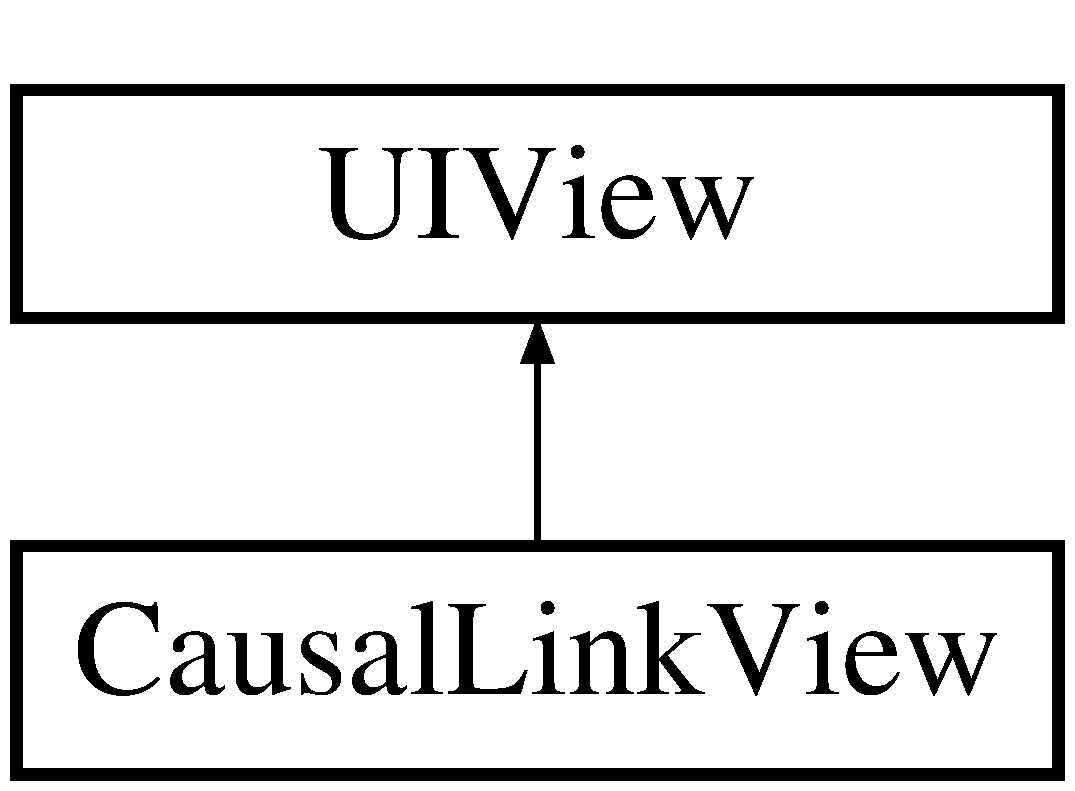
\includegraphics[height=2.000000cm]{interface_causal_link_view}
\end{center}
\end{figure}
\subsection*{Instance Methods}
\begin{DoxyCompactItemize}
\item 
(id) -\/ \hyperlink{interface_causal_link_view_af6c10f878fb1c7f420cc964aa0822992}{init\-With\-Parent\-:}
\item 
\hypertarget{interface_causal_link_view_aab9db45cbade40771ab30e01ff837142}{(void) -\/ \hyperlink{interface_causal_link_view_aab9db45cbade40771ab30e01ff837142}{init\-Member\-Vars}}\label{interface_causal_link_view_aab9db45cbade40771ab30e01ff837142}

\begin{DoxyCompactList}\small\item\em Initializes all of the member variables. \end{DoxyCompactList}\item 
(void) -\/ \hyperlink{interface_causal_link_view_a8c03538769a6fcbd7aa8e672cf4b5c96}{draw\-Rect\-:}
\item 
\hypertarget{interface_causal_link_view_a481c18609b8c7f6b790109ce163f0c5a}{(void) -\/ \hyperlink{interface_causal_link_view_a481c18609b8c7f6b790109ce163f0c5a}{draw\-Arc}}\label{interface_causal_link_view_a481c18609b8c7f6b790109ce163f0c5a}

\begin{DoxyCompactList}\small\item\em Draws the \hyperlink{interface_causal_link}{Causal\-Link} arc by creating a quad curve Bezier path. \end{DoxyCompactList}\item 
(void) -\/ \hyperlink{interface_causal_link_view_ad98cea31468b62d41184831cf9c779e1}{draw\-Arrowhead}
\item 
(void) -\/ \hyperlink{interface_causal_link_view_a59c2ffcd4e00222816f63842ed7311c0}{draw\-Time\-Delay}
\item 
(void) -\/ \hyperlink{interface_causal_link_view_ae80de0f1a90ac5fbc4cfada5278af48e}{draw\-Handle}
\item 
\hypertarget{interface_causal_link_view_abf9591a3ec825d59181114cc72560e3f}{(void) -\/ \hyperlink{interface_causal_link_view_abf9591a3ec825d59181114cc72560e3f}{draw\-Polarity}}\label{interface_causal_link_view_abf9591a3ec825d59181114cc72560e3f}

\begin{DoxyCompactList}\small\item\em Draws the polarity symbol (+, -\/) outside of the arc at the vertex. \end{DoxyCompactList}\item 
(float) -\/ \hyperlink{interface_causal_link_view_a12afbc746363f523651de2767d2487b2}{find\-Point\-On\-Quad\-Bezier\-Curve\-:p0\-:p1\-:p2\-:}
\item 
(C\-G\-Point) -\/ \hyperlink{interface_causal_link_view_a0493957fa8e8d0ec4f70d9b10321a604}{find\-Base\-Point\-:starting\-Tval\-:line\-Size\-:}
\item 
(C\-G\-Point) -\/ \hyperlink{interface_causal_link_view_a910e5f8e9cfba7c8881bf5555984996b}{rotate\-Line\-:base\-:degrees\-:}
\item 
(void) -\/ \hyperlink{interface_causal_link_view_a16ce7ec5c4dff09ffb1cfb9306977fc2}{calculate\-Frame}
\item 
(void) -\/ \hyperlink{interface_causal_link_view_afcd8e0f9b511eafba30829975f38f8b7}{move\-Arc\-:previous\-Location\-:}
\item 
(void) -\/ \hyperlink{interface_causal_link_view_a5ff220a0a810bec7f0eb1265fa10df73}{move\-Variable\-:modify\-Start\-Point\-:}
\item 
\hypertarget{interface_causal_link_view_a5e9eaa469086723dfe009fa52542ecd0}{(void) -\/ \hyperlink{interface_causal_link_view_a5e9eaa469086723dfe009fa52542ecd0}{calculate\-New\-Control\-Point}}\label{interface_causal_link_view_a5e9eaa469086723dfe009fa52542ecd0}

\begin{DoxyCompactList}\small\item\em Calculates a new control point because one of the variables related to the link has moved. \end{DoxyCompactList}\item 
\hypertarget{interface_causal_link_view_a1998df670fd8f6c2f22575522a4eab8a}{(void) -\/ \hyperlink{interface_causal_link_view_a1998df670fd8f6c2f22575522a4eab8a}{calculate\-Initial\-Arc}}\label{interface_causal_link_view_a1998df670fd8f6c2f22575522a4eab8a}

\begin{DoxyCompactList}\small\item\em Used on the initial import of the Vensim file. The .mdl file contains the handle location, but I handle all movement and the drawing of the causal links with a control point. I use the vertex point provided by the vensim file to calculate the inital control point and then any modification of the arc beyond this point will be handled by the control point. \end{DoxyCompactList}\item 
(C\-G\-Point) -\/ \hyperlink{interface_causal_link_view_afdedd2313a21ff2514c8f7c975e03f06}{find\-Point\-In\-Bounds\-:}
\item 
(void) -\/ \hyperlink{interface_causal_link_view_a339bfeabcfc5f19a0da1c941a6f70c8c}{resize\-Frame\-:new\-Origin\-:width\-:height\-:}
\item 
(void) -\/ \hyperlink{interface_causal_link_view_ace06597f5de275e1bb2a4d2d5b978e1f}{update\-Points\-In\-Frame\-:y\-Offset\-:}
\item 
(void) -\/ \hyperlink{interface_causal_link_view_a0d92c4b54808a5fa804ba5da408ec6a9}{update\-Slope}
\item 
(void) -\/ \hyperlink{interface_causal_link_view_a83f47d49615b69616f780c42780164c9}{update\-Vertex}
\item 
\hypertarget{interface_causal_link_view_a61a5c42146452337656a7abc21185686}{(void) -\/ \hyperlink{interface_causal_link_view_a61a5c42146452337656a7abc21185686}{update\-Link}}\label{interface_causal_link_view_a61a5c42146452337656a7abc21185686}

\begin{DoxyCompactList}\small\item\em Will make a call to create the menu of update options for the link. \end{DoxyCompactList}\item 
(B\-O\-O\-L) -\/ \hyperlink{interface_causal_link_view_af48e1d11b9394830d3c3b12a5f84ba61}{point\-Inside\-:with\-Event\-:}
\end{DoxyCompactItemize}
\subsection*{Class Methods}
\begin{DoxyCompactItemize}
\item 
(float) + \hyperlink{interface_causal_link_view_a23aef4b7c8b351589ca8e20f2a702bd0}{distance\-Between\-Points\-:second\-Point\-:}
\end{DoxyCompactItemize}
\subsection*{Properties}
\begin{DoxyCompactItemize}
\item 
\hypertarget{interface_causal_link_view_a8dbba850d3dff258b3106fac49e9bb6e}{U\-I\-Color $\ast$ \hyperlink{interface_causal_link_view_a8dbba850d3dff258b3106fac49e9bb6e}{arc\-Color}}\label{interface_causal_link_view_a8dbba850d3dff258b3106fac49e9bb6e}

\begin{DoxyCompactList}\small\item\em The color of the arc. \end{DoxyCompactList}\item 
\hypertarget{interface_causal_link_view_a323485e127244941fe6689cfbb2a2ac4}{bool \hyperlink{interface_causal_link_view_a323485e127244941fe6689cfbb2a2ac4}{is\-Bold}}\label{interface_causal_link_view_a323485e127244941fe6689cfbb2a2ac4}

\begin{DoxyCompactList}\small\item\em If the arc is bolded or not. \end{DoxyCompactList}\item 
\hypertarget{interface_causal_link_view_a2f7a630acc6a400de7beaf5689d5ab00}{bool \hyperlink{interface_causal_link_view_a2f7a630acc6a400de7beaf5689d5ab00}{has\-Time\-Delay}}\label{interface_causal_link_view_a2f7a630acc6a400de7beaf5689d5ab00}

\begin{DoxyCompactList}\small\item\em If the arc has a time delay. \end{DoxyCompactList}\item 
\hypertarget{interface_causal_link_view_aee10b0d74aca3ca6515a31d8c478f616}{C\-G\-Point \hyperlink{interface_causal_link_view_aee10b0d74aca3ca6515a31d8c478f616}{control\-Point}}\label{interface_causal_link_view_aee10b0d74aca3ca6515a31d8c478f616}

\begin{DoxyCompactList}\small\item\em The point at which the shape of the arc is controlled. \end{DoxyCompactList}\item 
\hypertarget{interface_causal_link_view_af5c8aa466e345adfab2e58ba5509edad}{C\-G\-Point \hyperlink{interface_causal_link_view_af5c8aa466e345adfab2e58ba5509edad}{start\-Point}}\label{interface_causal_link_view_af5c8aa466e345adfab2e58ba5509edad}

\begin{DoxyCompactList}\small\item\em The starting point of the arc. \end{DoxyCompactList}\item 
\hypertarget{interface_causal_link_view_a8182eda9bbf2964ae5df72b56cabffb0}{C\-G\-Point \hyperlink{interface_causal_link_view_a8182eda9bbf2964ae5df72b56cabffb0}{end\-Point}}\label{interface_causal_link_view_a8182eda9bbf2964ae5df72b56cabffb0}

\begin{DoxyCompactList}\small\item\em The ending point of the arc. \end{DoxyCompactList}\item 
\hypertarget{interface_causal_link_view_a77f66ca20ad3eb9bbcd3cfe1a99c0c62}{C\-G\-Point \hyperlink{interface_causal_link_view_a77f66ca20ad3eb9bbcd3cfe1a99c0c62}{vertex\-Point}}\label{interface_causal_link_view_a77f66ca20ad3eb9bbcd3cfe1a99c0c62}

\begin{DoxyCompactList}\small\item\em The vertex point of the arc. \end{DoxyCompactList}\item 
\hypertarget{interface_causal_link_view_a4376b99467d16ed71554a4a6ddd4ae0a}{id \hyperlink{interface_causal_link_view_a4376b99467d16ed71554a4a6ddd4ae0a}{parent}}\label{interface_causal_link_view_a4376b99467d16ed71554a4a6ddd4ae0a}

\begin{DoxyCompactList}\small\item\em Pointer to the parent of this view. \end{DoxyCompactList}\item 
\hypertarget{interface_causal_link_view_a90933fdc5eab518a50a919db52d55fc2}{N\-S\-String $\ast$ \hyperlink{interface_causal_link_view_a90933fdc5eab518a50a919db52d55fc2}{polarity}}\label{interface_causal_link_view_a90933fdc5eab518a50a919db52d55fc2}

\begin{DoxyCompactList}\small\item\em The type of causal link. + means that as one variable increases, so does the other. (ex. as a child eats more fast food, that child will gain more weight) -\/ means that as one variable increases, the other variable decreases. (ex. as a child eats healthier, the less weight gain will occur) \end{DoxyCompactList}\item 
\hypertarget{interface_causal_link_view_a556c38ae1a0c294ce33d9e3e40c656a4}{float \hyperlink{interface_causal_link_view_a556c38ae1a0c294ce33d9e3e40c656a4}{x\-Slope\-Change}}\label{interface_causal_link_view_a556c38ae1a0c294ce33d9e3e40c656a4}

\begin{DoxyCompactList}\small\item\em The slope in the x direction of the vertex point. \end{DoxyCompactList}\item 
\hypertarget{interface_causal_link_view_aaa52b4622b33e322e70bdc03892a38e7}{float \hyperlink{interface_causal_link_view_aaa52b4622b33e322e70bdc03892a38e7}{y\-Slope\-Change}}\label{interface_causal_link_view_aaa52b4622b33e322e70bdc03892a38e7}

\begin{DoxyCompactList}\small\item\em The slope in the y direction of the vertex point. \end{DoxyCompactList}\end{DoxyCompactItemize}


\subsection{Detailed Description}
A view that containg the graphical representation of a \hyperlink{interface_causal_link}{Causal\-Link}. 

\subsection{Method Documentation}
\hypertarget{interface_causal_link_view_a16ce7ec5c4dff09ffb1cfb9306977fc2}{\index{Causal\-Link\-View@{Causal\-Link\-View}!calculate\-Frame@{calculate\-Frame}}
\index{calculate\-Frame@{calculate\-Frame}!CausalLinkView@{Causal\-Link\-View}}
\subsubsection[{calculate\-Frame}]{\setlength{\rightskip}{0pt plus 5cm}-\/ (void) calculate\-Frame 
\begin{DoxyParamCaption}
{}
\end{DoxyParamCaption}
}}\label{interface_causal_link_view_a16ce7ec5c4dff09ffb1cfb9306977fc2}
Will calculate what the frame of the view should be based on where the three points of the arc are located. This method will then make a call to resize the frame and then update the points within the frame to take into account the changes. \hypertarget{interface_causal_link_view_a23aef4b7c8b351589ca8e20f2a702bd0}{\index{Causal\-Link\-View@{Causal\-Link\-View}!distance\-Between\-Points\-:second\-Point\-:@{distance\-Between\-Points\-:second\-Point\-:}}
\index{distance\-Between\-Points\-:second\-Point\-:@{distance\-Between\-Points\-:second\-Point\-:}!CausalLinkView@{Causal\-Link\-View}}
\subsubsection[{distance\-Between\-Points\-:second\-Point\-:}]{\setlength{\rightskip}{0pt plus 5cm}+ (float) distance\-Between\-Points\-: 
\begin{DoxyParamCaption}
\item[{(C\-G\-Point)}]{point1}
\item[{secondPoint:(C\-G\-Point)}]{point2}
\end{DoxyParamCaption}
}}\label{interface_causal_link_view_a23aef4b7c8b351589ca8e20f2a702bd0}
Determines the distance between two coordinate points using the standard distance formula. 
\begin{DoxyParams}{Parameters}
{\em point1} & the first coordinate point. \\
\hline
{\em point2} & the second coordinate point. \\
\hline
\end{DoxyParams}
\begin{DoxyReturn}{Returns}
the distance between point1 and point2. 
\end{DoxyReturn}
\hypertarget{interface_causal_link_view_ad98cea31468b62d41184831cf9c779e1}{\index{Causal\-Link\-View@{Causal\-Link\-View}!draw\-Arrowhead@{draw\-Arrowhead}}
\index{draw\-Arrowhead@{draw\-Arrowhead}!CausalLinkView@{Causal\-Link\-View}}
\subsubsection[{draw\-Arrowhead}]{\setlength{\rightskip}{0pt plus 5cm}-\/ (void) draw\-Arrowhead 
\begin{DoxyParamCaption}
{}
\end{DoxyParamCaption}
}}\label{interface_causal_link_view_ad98cea31468b62d41184831cf9c779e1}
Draws that arrowhead of the \hyperlink{interface_causal_link}{Causal\-Link}. To draw the arrow head, we follow the path of the bezier curve from the ending point, until it reaches a point outside the bounds of the view of the ending variable. This point is called the head of the arrow. Then we find a point further down the bezier curve that has a distance of A\-R\-R\-O\-W\-H\-E\-A\-D\-\_\-\-S\-I\-Z\-E from the head of the arrow. This point is called the base. Then the arrowhead will be drawn from these two points with a specified A\-R\-R\-O\-W\-H\-E\-A\-D\-\_\-\-A\-N\-G\-L\-E. \hypertarget{interface_causal_link_view_ae80de0f1a90ac5fbc4cfada5278af48e}{\index{Causal\-Link\-View@{Causal\-Link\-View}!draw\-Handle@{draw\-Handle}}
\index{draw\-Handle@{draw\-Handle}!CausalLinkView@{Causal\-Link\-View}}
\subsubsection[{draw\-Handle}]{\setlength{\rightskip}{0pt plus 5cm}-\/ (void) draw\-Handle 
\begin{DoxyParamCaption}
{}
\end{DoxyParamCaption}
}}\label{interface_causal_link_view_ae80de0f1a90ac5fbc4cfada5278af48e}
Draws the handle of the \hyperlink{interface_causal_link}{Causal\-Link}. The handle will be used to control the size of the arc. \hypertarget{interface_causal_link_view_a8c03538769a6fcbd7aa8e672cf4b5c96}{\index{Causal\-Link\-View@{Causal\-Link\-View}!draw\-Rect\-:@{draw\-Rect\-:}}
\index{draw\-Rect\-:@{draw\-Rect\-:}!CausalLinkView@{Causal\-Link\-View}}
\subsubsection[{draw\-Rect\-:}]{\setlength{\rightskip}{0pt plus 5cm}-\/ (void) draw\-Rect\-: 
\begin{DoxyParamCaption}
\item[{(C\-G\-Rect)}]{rect}
\end{DoxyParamCaption}
}}\label{interface_causal_link_view_a8c03538769a6fcbd7aa8e672cf4b5c96}
Draws the receiver’s image within the passed-\/in rectangle. This is an overridden method. 
\begin{DoxyParams}{Parameters}
{\em rect} & the frame of the view in which objects can be drawn. \\
\hline
\end{DoxyParams}
\hypertarget{interface_causal_link_view_a59c2ffcd4e00222816f63842ed7311c0}{\index{Causal\-Link\-View@{Causal\-Link\-View}!draw\-Time\-Delay@{draw\-Time\-Delay}}
\index{draw\-Time\-Delay@{draw\-Time\-Delay}!CausalLinkView@{Causal\-Link\-View}}
\subsubsection[{draw\-Time\-Delay}]{\setlength{\rightskip}{0pt plus 5cm}-\/ (void) draw\-Time\-Delay 
\begin{DoxyParamCaption}
{}
\end{DoxyParamCaption}
}}\label{interface_causal_link_view_a59c2ffcd4e00222816f63842ed7311c0}
Draws the time delay for the causal link if one exists. To draw this line the same algorithm is followed for drawing the arrowhead. We start at the vertex point and find another point along the curve of a specified size. Then we rotate the line to find two end points. We then use these two points to draw the line. \hypertarget{interface_causal_link_view_a0493957fa8e8d0ec4f70d9b10321a604}{\index{Causal\-Link\-View@{Causal\-Link\-View}!find\-Base\-Point\-:starting\-Tval\-:line\-Size\-:@{find\-Base\-Point\-:starting\-Tval\-:line\-Size\-:}}
\index{find\-Base\-Point\-:starting\-Tval\-:line\-Size\-:@{find\-Base\-Point\-:starting\-Tval\-:line\-Size\-:}!CausalLinkView@{Causal\-Link\-View}}
\subsubsection[{find\-Base\-Point\-:starting\-Tval\-:line\-Size\-:}]{\setlength{\rightskip}{0pt plus 5cm}-\/ (C\-G\-Point) find\-Base\-Point\-: 
\begin{DoxyParamCaption}
\item[{(C\-G\-Point)}]{head}
\item[{startingTval:(float)}]{t}
\item[{lineSize:(float)}]{size}
\end{DoxyParamCaption}
}}\label{interface_causal_link_view_a0493957fa8e8d0ec4f70d9b10321a604}
Will find the base coordinate point of the arrowhead. We want all arrowheads to be the same size and also want them to be perpendicular to the arc. In order to accomplish this, we follow the bezier arc path away from the head point of the arrowhead. We continue down the path until we reach the desired A\-R\-R\-O\-W\-H\-E\-A\-D\-\_\-\-S\-I\-Z\-E distance away from the head point. 
\begin{DoxyParams}{Parameters}
{\em head} & the coordinate location of the head of arrowhead. \\
\hline
{\em t} & the time parameter of the quad bezier curve equation to begin searching from. Should be set to the t value associated with the head of the arrow. \\
\hline
{\em size} & the size of the line you are looking for. \\
\hline
\end{DoxyParams}
\begin{DoxyReturn}{Returns}
a coordinate point that will serve as the base of the arrowhead. 
\end{DoxyReturn}
\hypertarget{interface_causal_link_view_afdedd2313a21ff2514c8f7c975e03f06}{\index{Causal\-Link\-View@{Causal\-Link\-View}!find\-Point\-In\-Bounds\-:@{find\-Point\-In\-Bounds\-:}}
\index{find\-Point\-In\-Bounds\-:@{find\-Point\-In\-Bounds\-:}!CausalLinkView@{Causal\-Link\-View}}
\subsubsection[{find\-Point\-In\-Bounds\-:}]{\setlength{\rightskip}{0pt plus 5cm}-\/ (C\-G\-Point) find\-Point\-In\-Bounds\-: 
\begin{DoxyParamCaption}
\item[{(C\-G\-Point)}]{ref\-Point}
\end{DoxyParamCaption}
}}\label{interface_causal_link_view_afdedd2313a21ff2514c8f7c975e03f06}
Used to compute new control and vertex points on the arc to make sure the arc will stay in bounds of the application. 
\begin{DoxyParams}{Parameters}
{\em ref\-Point} & the reference point that we are trying to modify. \\
\hline
\end{DoxyParams}
\begin{DoxyReturn}{Returns}
the new point location for the reference point. 
\end{DoxyReturn}
\hypertarget{interface_causal_link_view_a12afbc746363f523651de2767d2487b2}{\index{Causal\-Link\-View@{Causal\-Link\-View}!find\-Point\-On\-Quad\-Bezier\-Curve\-:p0\-:p1\-:p2\-:@{find\-Point\-On\-Quad\-Bezier\-Curve\-:p0\-:p1\-:p2\-:}}
\index{find\-Point\-On\-Quad\-Bezier\-Curve\-:p0\-:p1\-:p2\-:@{find\-Point\-On\-Quad\-Bezier\-Curve\-:p0\-:p1\-:p2\-:}!CausalLinkView@{Causal\-Link\-View}}
\subsubsection[{find\-Point\-On\-Quad\-Bezier\-Curve\-:p0\-:p1\-:p2\-:}]{\setlength{\rightskip}{0pt plus 5cm}-\/ (float) find\-Point\-On\-Quad\-Bezier\-Curve\-: 
\begin{DoxyParamCaption}
\item[{(float)}]{t}
\item[{p0:(float)}]{p0}
\item[{p1:(float)}]{p1}
\item[{p2:(float)}]{p2}
\end{DoxyParamCaption}
}}\label{interface_causal_link_view_a12afbc746363f523651de2767d2487b2}
Finds the x or y coordinate location on the quad bezier curve based on the value of t. Note that you will only pass all x coordinates or all y coordinates. You will not mix coordinates. Uses the equation B(t) = (1-\/t)$^\wedge$2 P0 + 2(1-\/t) $\ast$ t $\ast$ P1 + t$^\wedge$2 $\ast$ P2 
\begin{DoxyParams}{Parameters}
{\em t} & the time parameter. Will have a value between 0 and 1. \\
\hline
{\em p0} & the x or y coordinate of the starting\-Point on the bezier curve. \\
\hline
{\em p1} & the x or y coordinate of the control\-Point on the bezier curve. \\
\hline
{\em p2} & the x or y coordinate of the end\-Point on the bezier curve. \\
\hline
\end{DoxyParams}
\begin{DoxyReturn}{Returns}
the x or y coordinate of the coordinate point that lies along the bezier curve. 
\end{DoxyReturn}
\hypertarget{interface_causal_link_view_af6c10f878fb1c7f420cc964aa0822992}{\index{Causal\-Link\-View@{Causal\-Link\-View}!init\-With\-Parent\-:@{init\-With\-Parent\-:}}
\index{init\-With\-Parent\-:@{init\-With\-Parent\-:}!CausalLinkView@{Causal\-Link\-View}}
\subsubsection[{init\-With\-Parent\-:}]{\setlength{\rightskip}{0pt plus 5cm}-\/ (id) init\-With\-Parent\-: 
\begin{DoxyParamCaption}
\item[{(id)}]{parent}
\end{DoxyParamCaption}
}}\label{interface_causal_link_view_af6c10f878fb1c7f420cc964aa0822992}
Initializes the view. 
\begin{DoxyParams}{Parameters}
{\em parent} & a pointer to the parent object that holds the view. \\
\hline
\end{DoxyParams}
\begin{DoxyReturn}{Returns}
an id of the newly created view. 
\end{DoxyReturn}
\hypertarget{interface_causal_link_view_afcd8e0f9b511eafba30829975f38f8b7}{\index{Causal\-Link\-View@{Causal\-Link\-View}!move\-Arc\-:previous\-Location\-:@{move\-Arc\-:previous\-Location\-:}}
\index{move\-Arc\-:previous\-Location\-:@{move\-Arc\-:previous\-Location\-:}!CausalLinkView@{Causal\-Link\-View}}
\subsubsection[{move\-Arc\-:previous\-Location\-:}]{\setlength{\rightskip}{0pt plus 5cm}-\/ (void) move\-Arc\-: 
\begin{DoxyParamCaption}
\item[{(C\-G\-Point)}]{location}
\item[{previousLocation:(C\-G\-Point)}]{prev\-Location}
\end{DoxyParamCaption}
}}\label{interface_causal_link_view_afcd8e0f9b511eafba30829975f38f8b7}
Will handle the moving of the arc up and down. After modifiying the control point, a method call will be made to adjust the frame. 
\begin{DoxyParams}{Parameters}
{\em location} & the coordinate location of where the user's finger is located. \\
\hline
{\em prev\-Location} & the coordinate location of where the user's finger use to be located. \\
\hline
\end{DoxyParams}
\hypertarget{interface_causal_link_view_a5ff220a0a810bec7f0eb1265fa10df73}{\index{Causal\-Link\-View@{Causal\-Link\-View}!move\-Variable\-:modify\-Start\-Point\-:@{move\-Variable\-:modify\-Start\-Point\-:}}
\index{move\-Variable\-:modify\-Start\-Point\-:@{move\-Variable\-:modify\-Start\-Point\-:}!CausalLinkView@{Causal\-Link\-View}}
\subsubsection[{move\-Variable\-:modify\-Start\-Point\-:}]{\setlength{\rightskip}{0pt plus 5cm}-\/ (void) move\-Variable\-: 
\begin{DoxyParamCaption}
\item[{(C\-G\-Point)}]{new\-Center}
\item[{modifyStartPoint:(bool)}]{is\-Start\-Point}
\end{DoxyParamCaption}
}}\label{interface_causal_link_view_a5ff220a0a810bec7f0eb1265fa10df73}
This method updates the arc when either the starting or ending point variable has moved. 
\begin{DoxyParams}{Parameters}
{\em new\-Center} & the center point location of the variable that moved. \\
\hline
{\em is\-Start\-Point} & whether or not the variable that changed was the start\-Point. \\
\hline
\end{DoxyParams}
\hypertarget{interface_causal_link_view_af48e1d11b9394830d3c3b12a5f84ba61}{\index{Causal\-Link\-View@{Causal\-Link\-View}!point\-Inside\-:with\-Event\-:@{point\-Inside\-:with\-Event\-:}}
\index{point\-Inside\-:with\-Event\-:@{point\-Inside\-:with\-Event\-:}!CausalLinkView@{Causal\-Link\-View}}
\subsubsection[{point\-Inside\-:with\-Event\-:}]{\setlength{\rightskip}{0pt plus 5cm}-\/ (B\-O\-O\-L) point\-Inside\-: 
\begin{DoxyParamCaption}
\item[{(C\-G\-Point)}]{point}
\item[{withEvent:(U\-I\-Event $\ast$)}]{event}
\end{DoxyParamCaption}
}}\label{interface_causal_link_view_af48e1d11b9394830d3c3b12a5f84ba61}
Will allow any of the children of the view to receive touches but the view itself will be transparent to events. 
\begin{DoxyParams}{Parameters}
{\em point} & the point where the event occurred. \\
\hline
{\em event} & the associated event initiated by the user. \\
\hline
\end{DoxyParams}
\begin{DoxyReturn}{Returns}
whether or not this view handled the event. 
\end{DoxyReturn}
\hypertarget{interface_causal_link_view_a339bfeabcfc5f19a0da1c941a6f70c8c}{\index{Causal\-Link\-View@{Causal\-Link\-View}!resize\-Frame\-:new\-Origin\-:width\-:height\-:@{resize\-Frame\-:new\-Origin\-:width\-:height\-:}}
\index{resize\-Frame\-:new\-Origin\-:width\-:height\-:@{resize\-Frame\-:new\-Origin\-:width\-:height\-:}!CausalLinkView@{Causal\-Link\-View}}
\subsubsection[{resize\-Frame\-:new\-Origin\-:width\-:height\-:}]{\setlength{\rightskip}{0pt plus 5cm}-\/ (void) resize\-Frame\-: 
\begin{DoxyParamCaption}
\item[{(C\-G\-Point)}]{old\-Origin}
\item[{newOrigin:(C\-G\-Point)}]{new\-Origin}
\item[{width:(float)}]{size\-Width}
\item[{height:(float)}]{size\-Height}
\end{DoxyParamCaption}
}}\label{interface_causal_link_view_a339bfeabcfc5f19a0da1c941a6f70c8c}
Will set the frame based on the given parameters. Will determine what the transalation of the old frame and the new frame is and then will make a method call to update all of the points within the frame. 
\begin{DoxyParams}{Parameters}
{\em old\-Origin} & the old origin of the frame. \\
\hline
{\em new\-Origin} & the new origin of the frame. \\
\hline
{\em size\-Width} & the new width of the frame. \\
\hline
{\em size\-Height} & the new height of the frame. \\
\hline
\end{DoxyParams}
\hypertarget{interface_causal_link_view_a910e5f8e9cfba7c8881bf5555984996b}{\index{Causal\-Link\-View@{Causal\-Link\-View}!rotate\-Line\-:base\-:degrees\-:@{rotate\-Line\-:base\-:degrees\-:}}
\index{rotate\-Line\-:base\-:degrees\-:@{rotate\-Line\-:base\-:degrees\-:}!CausalLinkView@{Causal\-Link\-View}}
\subsubsection[{rotate\-Line\-:base\-:degrees\-:}]{\setlength{\rightskip}{0pt plus 5cm}-\/ (C\-G\-Point) rotate\-Line\-: 
\begin{DoxyParamCaption}
\item[{(C\-G\-Point)}]{head}
\item[{base:(C\-G\-Point)}]{base}
\item[{degrees:(float)}]{degrees}
\end{DoxyParamCaption}
}}\label{interface_causal_link_view_a910e5f8e9cfba7c8881bf5555984996b}
This will rotate the line that extends from the head point to the base point by a passed in number of degrees. This method is used to find the corner points of the arrowhead by utilizing a linear algebra rotation matrix to perform rotation in Euclidian space. 
\begin{DoxyParams}{Parameters}
{\em head} & the head point of the arrowhead. \\
\hline
{\em base} & the base point of the arrowhead. \\
\hline
{\em degrees} & the number of degree we would like to rotate the line from the head to the base to get the corner point of the arrow. \\
\hline
\end{DoxyParams}
\begin{DoxyReturn}{Returns}
the corner point of the rotated line, that is rotated around the head point. 
\end{DoxyReturn}
\hypertarget{interface_causal_link_view_ace06597f5de275e1bb2a4d2d5b978e1f}{\index{Causal\-Link\-View@{Causal\-Link\-View}!update\-Points\-In\-Frame\-:y\-Offset\-:@{update\-Points\-In\-Frame\-:y\-Offset\-:}}
\index{update\-Points\-In\-Frame\-:y\-Offset\-:@{update\-Points\-In\-Frame\-:y\-Offset\-:}!CausalLinkView@{Causal\-Link\-View}}
\subsubsection[{update\-Points\-In\-Frame\-:y\-Offset\-:}]{\setlength{\rightskip}{0pt plus 5cm}-\/ (void) update\-Points\-In\-Frame\-: 
\begin{DoxyParamCaption}
\item[{(float)}]{x\-Offset}
\item[{yOffset:(float)}]{y\-Offset}
\end{DoxyParamCaption}
}}\label{interface_causal_link_view_ace06597f5de275e1bb2a4d2d5b978e1f}
Will translate all of the points in the frame based on the offset of the frame changes. 
\begin{DoxyParams}{Parameters}
{\em x\-Offset} & the change in the x coordinate between the old and new frames. \\
\hline
{\em y\-Offset} & the change in the y coordinate between the old and new frames. \\
\hline
\end{DoxyParams}
\hypertarget{interface_causal_link_view_a0d92c4b54808a5fa804ba5da408ec6a9}{\index{Causal\-Link\-View@{Causal\-Link\-View}!update\-Slope@{update\-Slope}}
\index{update\-Slope@{update\-Slope}!CausalLinkView@{Causal\-Link\-View}}
\subsubsection[{update\-Slope}]{\setlength{\rightskip}{0pt plus 5cm}-\/ (void) update\-Slope 
\begin{DoxyParamCaption}
{}
\end{DoxyParamCaption}
}}\label{interface_causal_link_view_a0d92c4b54808a5fa804ba5da408ec6a9}
This will update the slope of the arc. It will iteratively decrease the size of the slope until it is within range of normal movement of a finger gesture. \hypertarget{interface_causal_link_view_a83f47d49615b69616f780c42780164c9}{\index{Causal\-Link\-View@{Causal\-Link\-View}!update\-Vertex@{update\-Vertex}}
\index{update\-Vertex@{update\-Vertex}!CausalLinkView@{Causal\-Link\-View}}
\subsubsection[{update\-Vertex}]{\setlength{\rightskip}{0pt plus 5cm}-\/ (void) update\-Vertex 
\begin{DoxyParamCaption}
{}
\end{DoxyParamCaption}
}}\label{interface_causal_link_view_a83f47d49615b69616f780c42780164c9}
This method will recompute the vertex based on the starting point, ending point, and control point. This method should be called any time any one of the three points moves. 

The documentation for this class was generated from the following files\-:\begin{DoxyCompactItemize}
\item 
Group\-Modeling\-App/Causal\-Link\-View.\-h\item 
Group\-Modeling\-App/Causal\-Link\-View.\-m\end{DoxyCompactItemize}

\hypertarget{interface_component}{\section{Component Class Reference}
\label{interface_component}\index{Component@{Component}}
}


A superclass that holds all generic data about all objects in the causal diagram model.  




{\ttfamily \#import $<$Component.\-h$>$}

Inheritance diagram for Component\-:\begin{figure}[H]
\begin{center}
\leavevmode
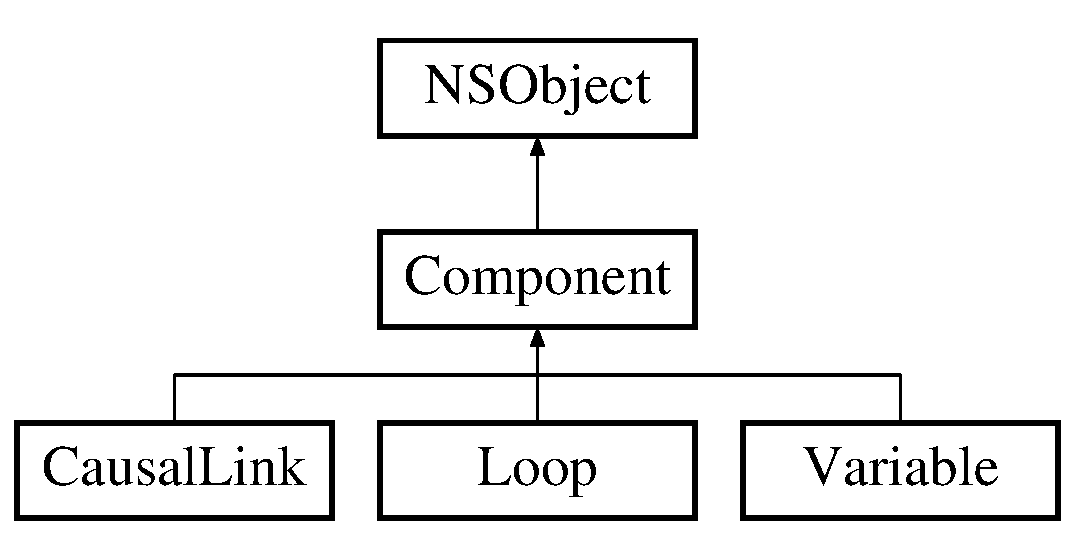
\includegraphics[height=3.000000cm]{interface_component}
\end{center}
\end{figure}
\subsection*{Instance Methods}
\begin{DoxyCompactItemize}
\item 
\hypertarget{interface_component_a4213bb26f5207ee3f402fe463badc691}{(id) -\/ {\bfseries init}}\label{interface_component_a4213bb26f5207ee3f402fe463badc691}

\end{DoxyCompactItemize}
\subsection*{Class Methods}
\begin{DoxyCompactItemize}
\item 
(int) + \hyperlink{interface_component_a3d13675a50c2e37e16e1b7858e5510e4}{generate\-I\-D}
\item 
\hypertarget{interface_component_a729723fbabf97aacfb842008ac0a354a}{(void) + \hyperlink{interface_component_a729723fbabf97aacfb842008ac0a354a}{reset\-I\-D\-Counter}}\label{interface_component_a729723fbabf97aacfb842008ac0a354a}

\begin{DoxyCompactList}\small\item\em Called to set the id counter back to zero when either a new file is created or opened. \end{DoxyCompactList}\item 
(int) + \hyperlink{interface_component_a5dd925a5e48c04cad74e8beb21d293ff}{get\-Largest\-I\-D\-Num}
\item 
(void) + \hyperlink{interface_component_ae07661532eb80738c2008859e8a198b7}{set\-Largest\-I\-D\-Num\-:}
\item 
(N\-S\-String $\ast$) + \hyperlink{interface_component_a875d9dcfa3e019c2cf685524707e0427}{sanitize\-String\-:}
\end{DoxyCompactItemize}
\subsection*{Properties}
\begin{DoxyCompactItemize}
\item 
\hypertarget{interface_component_aa1014a20b8eef81a91c90ed7740d4a10}{int \hyperlink{interface_component_aa1014a20b8eef81a91c90ed7740d4a10}{id\-Num}}\label{interface_component_aa1014a20b8eef81a91c90ed7740d4a10}

\begin{DoxyCompactList}\small\item\em The id number of the component in the model. This should be unique for every instance of the component in the model. \end{DoxyCompactList}\item 
\hypertarget{interface_component_ab15484f6d515849f3363dd48a9aea09a}{int \hyperlink{interface_component_ab15484f6d515849f3363dd48a9aea09a}{object\-Type}}\label{interface_component_ab15484f6d515849f3363dd48a9aea09a}

\begin{DoxyCompactList}\small\item\em Specifiying the type of the object. Should be a \hyperlink{interface_variable}{Variable} = 10, \hyperlink{interface_causal_link}{Causal\-Link} = 1, or a \hyperlink{interface_loop}{Loop} = 12. \end{DoxyCompactList}\end{DoxyCompactItemize}


\subsection{Detailed Description}
A superclass that holds all generic data about all objects in the causal diagram model. 

\subsection{Method Documentation}
\hypertarget{interface_component_a3d13675a50c2e37e16e1b7858e5510e4}{\index{Component@{Component}!generate\-I\-D@{generate\-I\-D}}
\index{generate\-I\-D@{generate\-I\-D}!Component@{Component}}
\subsubsection[{generate\-I\-D}]{\setlength{\rightskip}{0pt plus 5cm}+ (int) generate\-I\-D 
\begin{DoxyParamCaption}
{}
\end{DoxyParamCaption}
}}\label{interface_component_a3d13675a50c2e37e16e1b7858e5510e4}
\begin{DoxyRefDesc}{Todo}
\item[\hyperlink{todo__todo000001}{Todo}]would be nice to remove this static variable Called for every subclass instance to keep track of how many objects there are currently in the model. The main use of this method will be to generate identification numbers for newly created objects by the user. Should only be called once by the component model in the init. \end{DoxyRefDesc}
\begin{DoxyReturn}{Returns}
the unique id number for the component. 
\end{DoxyReturn}
\hypertarget{interface_component_a5dd925a5e48c04cad74e8beb21d293ff}{\index{Component@{Component}!get\-Largest\-I\-D\-Num@{get\-Largest\-I\-D\-Num}}
\index{get\-Largest\-I\-D\-Num@{get\-Largest\-I\-D\-Num}!Component@{Component}}
\subsubsection[{get\-Largest\-I\-D\-Num}]{\setlength{\rightskip}{0pt plus 5cm}+ (int) get\-Largest\-I\-D\-Num 
\begin{DoxyParamCaption}
{}
\end{DoxyParamCaption}
}}\label{interface_component_a5dd925a5e48c04cad74e8beb21d293ff}
Returns the largest id number. \begin{DoxyReturn}{Returns}
the largest id number which will be the value of id\-Iter. 
\end{DoxyReturn}
\hypertarget{interface_component_a875d9dcfa3e019c2cf685524707e0427}{\index{Component@{Component}!sanitize\-String\-:@{sanitize\-String\-:}}
\index{sanitize\-String\-:@{sanitize\-String\-:}!Component@{Component}}
\subsubsection[{sanitize\-String\-:}]{\setlength{\rightskip}{0pt plus 5cm}+ (N\-S\-String$\ast$) sanitize\-String\-: 
\begin{DoxyParamCaption}
\item[{(N\-S\-String $\ast$)}]{str}
\end{DoxyParamCaption}
}}\label{interface_component_a875d9dcfa3e019c2cf685524707e0427}
\begin{DoxyRefDesc}{Todo}
\item[\hyperlink{todo__todo000002}{Todo}]For some reason string\-By\-Replacing\-Occurrences\-Of\-String causes Doxygen to not be able to find the .m file. So i have documentation duplicated in both files right now... Used to sanitize strings that may contain extraneous escape characters. \end{DoxyRefDesc}

\begin{DoxyParams}{Parameters}
{\em str} & the string that needs to be returned. \\
\hline
\end{DoxyParams}
\begin{DoxyReturn}{Returns}
a string that does not contain any extra backslashes or double-\/quotes. 
\end{DoxyReturn}
\hypertarget{interface_component_ae07661532eb80738c2008859e8a198b7}{\index{Component@{Component}!set\-Largest\-I\-D\-Num\-:@{set\-Largest\-I\-D\-Num\-:}}
\index{set\-Largest\-I\-D\-Num\-:@{set\-Largest\-I\-D\-Num\-:}!Component@{Component}}
\subsubsection[{set\-Largest\-I\-D\-Num\-:}]{\setlength{\rightskip}{0pt plus 5cm}+ (void) set\-Largest\-I\-D\-Num\-: 
\begin{DoxyParamCaption}
\item[{(int)}]{num}
\end{DoxyParamCaption}
}}\label{interface_component_ae07661532eb80738c2008859e8a198b7}
Sets the id\-Iter to the current largest id num on import. 
\begin{DoxyParams}{Parameters}
{\em num} & the largest id number. \\
\hline
\end{DoxyParams}


The documentation for this class was generated from the following file\-:\begin{DoxyCompactItemize}
\item 
Group\-Modeling\-App/Component.\-h\end{DoxyCompactItemize}

\hypertarget{interface_control_parameters}{\section{Control\-Parameters Class Reference}
\label{interface_control_parameters}\index{Control\-Parameters@{Control\-Parameters}}
}


This class currently holds an array with the control parameters, but was created to allow for expansion if we would want to parse the array into its individual control parameters and be able to update them individually.  




{\ttfamily \#import $<$Control\-Parameters.\-h$>$}

Inheritance diagram for Control\-Parameters\-:\begin{figure}[H]
\begin{center}
\leavevmode
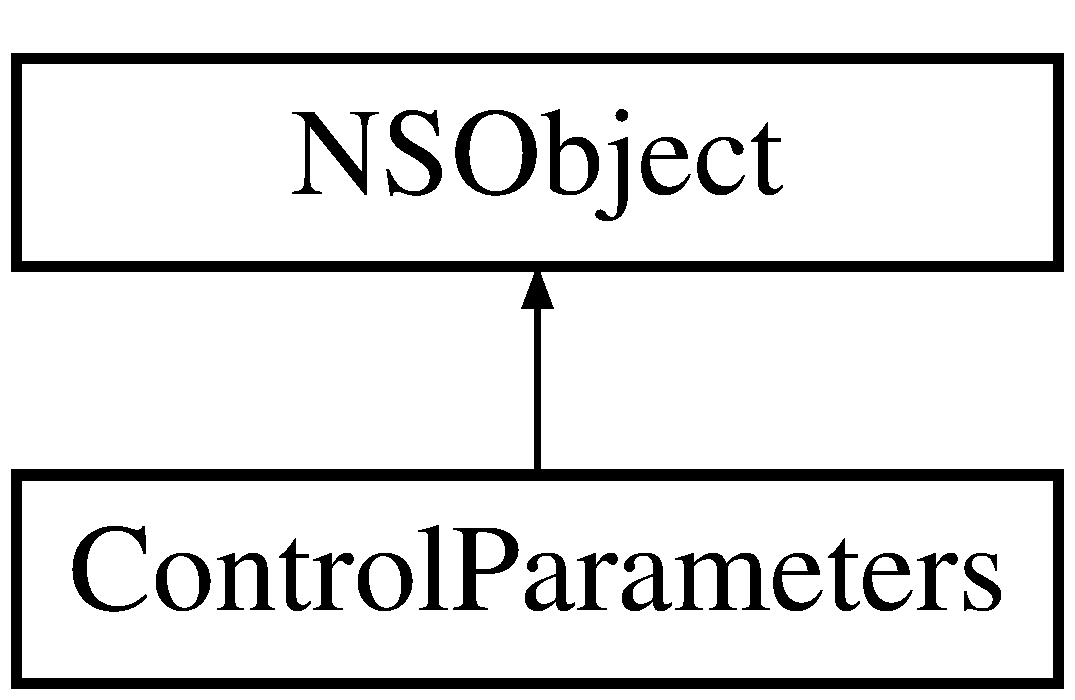
\includegraphics[height=2.000000cm]{interface_control_parameters}
\end{center}
\end{figure}
\subsection*{Instance Methods}
\begin{DoxyCompactItemize}
\item 
(id) -\/ \hyperlink{interface_control_parameters_a4213bb26f5207ee3f402fe463badc691}{init}
\item 
(void) -\/ \hyperlink{interface_control_parameters_ab0bbfe8242a098b77c936f8a10df7947}{add\-Parameter\-:}
\end{DoxyCompactItemize}
\subsection*{Properties}
\begin{DoxyCompactItemize}
\item 
\hypertarget{interface_control_parameters_aa66ff297704a6ceeb0b02d1421d9a2c4}{N\-S\-Mutable\-Array $\ast$ \hyperlink{interface_control_parameters_aa66ff297704a6ceeb0b02d1421d9a2c4}{params}}\label{interface_control_parameters_aa66ff297704a6ceeb0b02d1421d9a2c4}

\begin{DoxyCompactList}\small\item\em An array containing all of the simulation control parameters. \end{DoxyCompactList}\end{DoxyCompactItemize}


\subsection{Detailed Description}
This class currently holds an array with the control parameters, but was created to allow for expansion if we would want to parse the array into its individual control parameters and be able to update them individually. 

\subsection{Method Documentation}
\hypertarget{interface_control_parameters_ab0bbfe8242a098b77c936f8a10df7947}{\index{Control\-Parameters@{Control\-Parameters}!add\-Parameter\-:@{add\-Parameter\-:}}
\index{add\-Parameter\-:@{add\-Parameter\-:}!ControlParameters@{Control\-Parameters}}
\subsubsection[{add\-Parameter\-:}]{\setlength{\rightskip}{0pt plus 5cm}-\/ (void) add\-Parameter\-: 
\begin{DoxyParamCaption}
\item[{(N\-S\-String$\ast$)}]{str}
\end{DoxyParamCaption}
}}\label{interface_control_parameters_ab0bbfe8242a098b77c936f8a10df7947}
Adds a new string of the control parameters to the params array. 
\begin{DoxyParams}{Parameters}
{\em str} & a string of the control parameters to be appended to the existing simulation control parameters. \\
\hline
\end{DoxyParams}
\hypertarget{interface_control_parameters_a4213bb26f5207ee3f402fe463badc691}{\index{Control\-Parameters@{Control\-Parameters}!init@{init}}
\index{init@{init}!ControlParameters@{Control\-Parameters}}
\subsubsection[{init}]{\setlength{\rightskip}{0pt plus 5cm}-\/ (id) init 
\begin{DoxyParamCaption}
{}
\end{DoxyParamCaption}
}}\label{interface_control_parameters_a4213bb26f5207ee3f402fe463badc691}
Initializes the \hyperlink{interface_control_parameters}{Control\-Parameters}. \begin{DoxyReturn}{Returns}
a pointer to the newly created \hyperlink{interface_control_parameters}{Control\-Parameters} object. 
\end{DoxyReturn}


The documentation for this class was generated from the following files\-:\begin{DoxyCompactItemize}
\item 
Group\-Modeling\-App/Control\-Parameters.\-h\item 
Group\-Modeling\-App/Control\-Parameters.\-m\end{DoxyCompactItemize}

\hypertarget{interface_default_parameters}{\section{Default\-Parameters Class Reference}
\label{interface_default_parameters}\index{Default\-Parameters@{Default\-Parameters}}
}


This class currently holds a string with the default parameters, but was created to allow for expansion if we would want to parse the string into its individual pieces and be able to update them individually.  




{\ttfamily \#import $<$Default\-Parameters.\-h$>$}

Inheritance diagram for Default\-Parameters\-:\begin{figure}[H]
\begin{center}
\leavevmode
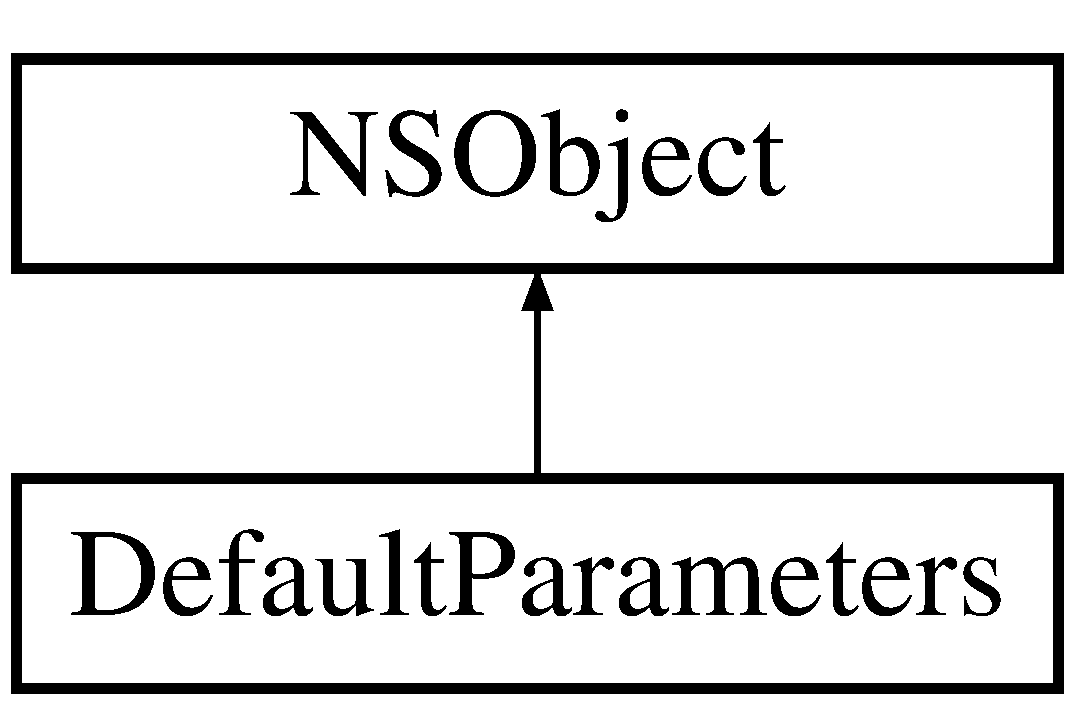
\includegraphics[height=2.000000cm]{interface_default_parameters}
\end{center}
\end{figure}
\subsection*{Instance Methods}
\begin{DoxyCompactItemize}
\item 
(id) -\/ \hyperlink{interface_default_parameters_a56118e230ce34a2601faf5c95a358cb6}{init\-:}
\end{DoxyCompactItemize}
\subsection*{Properties}
\begin{DoxyCompactItemize}
\item 
\hypertarget{interface_default_parameters_aebb372b87de453d373aac55ecddc6303}{N\-S\-String $\ast$ \hyperlink{interface_default_parameters_aebb372b87de453d373aac55ecddc6303}{params}}\label{interface_default_parameters_aebb372b87de453d373aac55ecddc6303}

\begin{DoxyCompactList}\small\item\em A string containing all of the default parameters including font, and size. \end{DoxyCompactList}\end{DoxyCompactItemize}


\subsection{Detailed Description}
This class currently holds a string with the default parameters, but was created to allow for expansion if we would want to parse the string into its individual pieces and be able to update them individually. 

\subsection{Method Documentation}
\hypertarget{interface_default_parameters_a56118e230ce34a2601faf5c95a358cb6}{\index{Default\-Parameters@{Default\-Parameters}!init\-:@{init\-:}}
\index{init\-:@{init\-:}!DefaultParameters@{Default\-Parameters}}
\subsubsection[{init\-:}]{\setlength{\rightskip}{0pt plus 5cm}-\/ (id) init\-: 
\begin{DoxyParamCaption}
\item[{(N\-S\-String$\ast$)}]{data}
\end{DoxyParamCaption}
}}\label{interface_default_parameters_a56118e230ce34a2601faf5c95a358cb6}
Initializes the \hyperlink{interface_default_parameters}{Default\-Parameters}. 
\begin{DoxyParams}{Parameters}
{\em data} & the string of data containing the default parameters of the model. \\
\hline
\end{DoxyParams}
\begin{DoxyReturn}{Returns}
a pointer to the newly created \hyperlink{interface_default_parameters}{Default\-Parameters} object. 
\end{DoxyReturn}


The documentation for this class was generated from the following files\-:\begin{DoxyCompactItemize}
\item 
Group\-Modeling\-App/Default\-Parameters.\-h\item 
Group\-Modeling\-App/Default\-Parameters.\-m\end{DoxyCompactItemize}

\hypertarget{interface_detailed_help_section_view_controller}{\section{Detailed\-Help\-Section\-View\-Controller Class Reference}
\label{interface_detailed_help_section_view_controller}\index{Detailed\-Help\-Section\-View\-Controller@{Detailed\-Help\-Section\-View\-Controller}}
}
Inheritance diagram for Detailed\-Help\-Section\-View\-Controller\-:\begin{figure}[H]
\begin{center}
\leavevmode
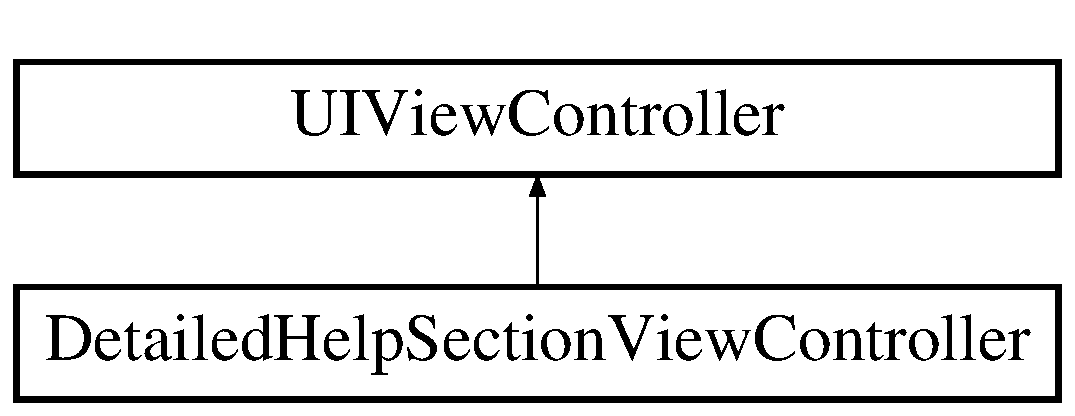
\includegraphics[height=2.000000cm]{interface_detailed_help_section_view_controller}
\end{center}
\end{figure}


The documentation for this class was generated from the following file\-:\begin{DoxyCompactItemize}
\item 
Group\-Modeling\-App/Detailed\-Help\-Section\-View\-Controller.\-h\end{DoxyCompactItemize}

\hypertarget{category_detailed_help_section_view_controller_07_08}{\section{Detailed\-Help\-Section\-View\-Controller() Category Reference}
\label{category_detailed_help_section_view_controller_07_08}\index{Detailed\-Help\-Section\-View\-Controller()@{Detailed\-Help\-Section\-View\-Controller()}}
}


The documentation for this category was generated from the following file\-:\begin{DoxyCompactItemize}
\item 
Group\-Modeling\-App/Detailed\-Help\-Section\-View\-Controller.\-m\end{DoxyCompactItemize}

\hypertarget{interface_event}{\section{Event Class Reference}
\label{interface_event}\index{Event@{Event}}
}


A class used to construct events that occur in the simulation.  




{\ttfamily \#import $<$Event.\-h$>$}

Inheritance diagram for Event\-:\begin{figure}[H]
\begin{center}
\leavevmode
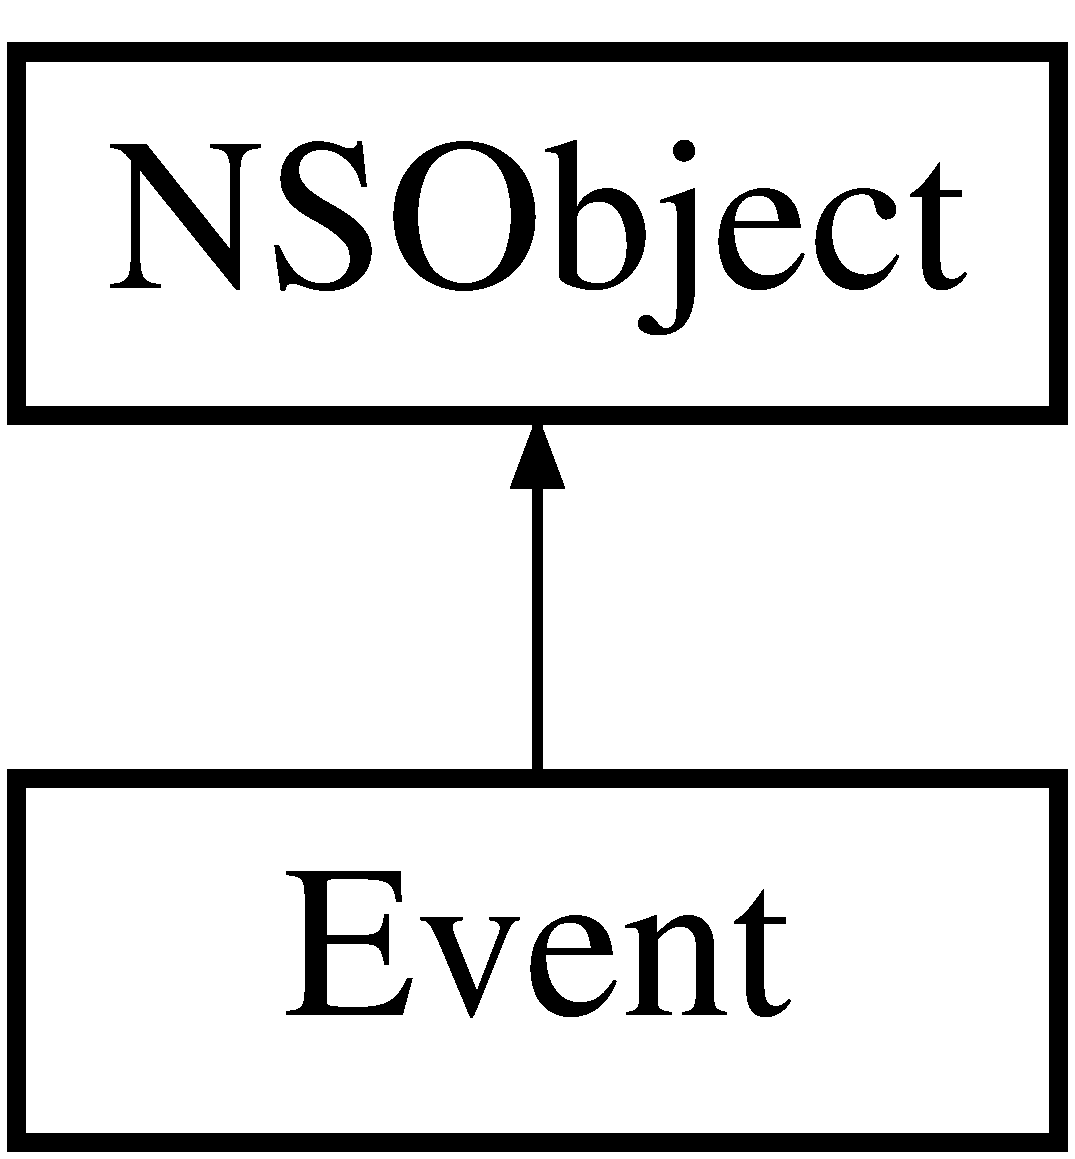
\includegraphics[height=2.000000cm]{interface_event}
\end{center}
\end{figure}
\subsection*{Instance Methods}
\begin{DoxyCompactItemize}
\item 
(id) -\/ \hyperlink{interface_event_a9f84a217411ee0ffbaa3def1332ec8bd}{init\-With\-Desc\-I\-D\-:}
\item 
(id) -\/ \hyperlink{interface_event_ae719cd1948e9cfa11caf1eea81012b4c}{init\-With\-Desc\-I\-D\-:and\-Object\-I\-D\-:}
\item 
(id) -\/ \hyperlink{interface_event_ae0b25c192d084ad864831170aac1d542}{init\-With\-Desc\-I\-D\-:and\-Details\-:}
\item 
(id) -\/ \hyperlink{interface_event_ae185f9bf45394b5d54c542085c91b133}{init\-With\-Desc\-I\-D\-:and\-Object\-I\-D\-:and\-Details\-:}
\end{DoxyCompactItemize}
\subsection*{Properties}
\begin{DoxyCompactItemize}
\item 
\hypertarget{interface_event_a7999a182561543e6f8a6b11633fdf26f}{N\-S\-Number $\ast$ \hyperlink{interface_event_a7999a182561543e6f8a6b11633fdf26f}{time}}\label{interface_event_a7999a182561543e6f8a6b11633fdf26f}

\begin{DoxyCompactList}\small\item\em The time the event occurred. \end{DoxyCompactList}\item 
\hypertarget{interface_event_aecb5d4221768a4af5d82df3420a25339}{int \hyperlink{interface_event_aecb5d4221768a4af5d82df3420a25339}{description\-I\-D}}\label{interface_event_aecb5d4221768a4af5d82df3420a25339}

\begin{DoxyCompactList}\small\item\em The id number of the generic event. \end{DoxyCompactList}\item 
\hypertarget{interface_event_a32f790016241cf78c44782a6007a744f}{int \hyperlink{interface_event_a32f790016241cf78c44782a6007a744f}{object\-I\-D}}\label{interface_event_a32f790016241cf78c44782a6007a744f}

\begin{DoxyCompactList}\small\item\em The id number of the object that was affected by the change. \end{DoxyCompactList}\item 
\hypertarget{interface_event_a8fc6cd2b92f759c4e2a74e32d615e4dd}{N\-S\-String $\ast$ \hyperlink{interface_event_a8fc6cd2b92f759c4e2a74e32d615e4dd}{details}}\label{interface_event_a8fc6cd2b92f759c4e2a74e32d615e4dd}

\begin{DoxyCompactList}\small\item\em Any details regarding the change. \end{DoxyCompactList}\end{DoxyCompactItemize}


\subsection{Detailed Description}
A class used to construct events that occur in the simulation. 

\subsection{Method Documentation}
\hypertarget{interface_event_a9f84a217411ee0ffbaa3def1332ec8bd}{\index{Event@{Event}!init\-With\-Desc\-I\-D\-:@{init\-With\-Desc\-I\-D\-:}}
\index{init\-With\-Desc\-I\-D\-:@{init\-With\-Desc\-I\-D\-:}!Event@{Event}}
\subsubsection[{init\-With\-Desc\-I\-D\-:}]{\setlength{\rightskip}{0pt plus 5cm}-\/ (id) init\-With\-Desc\-I\-D\-: 
\begin{DoxyParamCaption}
\item[{(int)}]{desc\-I\-D}
\end{DoxyParamCaption}
}}\label{interface_event_a9f84a217411ee0ffbaa3def1332ec8bd}
Initializes the \hyperlink{interface_event}{Event} given the description id. Will fill in the other aspects of the class with defaults. Calls init\-With\-Desc\-I\-D\-: and\-Object\-I\-D\-: and\-Details\-:. 
\begin{DoxyParams}{Parameters}
{\em desc\-I\-D} & the identification number of the generic description message. \\
\hline
\end{DoxyParams}
\begin{DoxyReturn}{Returns}
a pointer to the event object. 
\end{DoxyReturn}
\hypertarget{interface_event_ae0b25c192d084ad864831170aac1d542}{\index{Event@{Event}!init\-With\-Desc\-I\-D\-:and\-Details\-:@{init\-With\-Desc\-I\-D\-:and\-Details\-:}}
\index{init\-With\-Desc\-I\-D\-:and\-Details\-:@{init\-With\-Desc\-I\-D\-:and\-Details\-:}!Event@{Event}}
\subsubsection[{init\-With\-Desc\-I\-D\-:and\-Details\-:}]{\setlength{\rightskip}{0pt plus 5cm}-\/ (id) {\bf init\-With\-Desc\-I\-D\-:} 
\begin{DoxyParamCaption}
\item[{(int)}]{desc\-I\-D}
\item[{andDetails:(N\-S\-String$\ast$)}]{details}
\end{DoxyParamCaption}
}}\label{interface_event_ae0b25c192d084ad864831170aac1d542}
Initializes the \hyperlink{interface_event}{Event} given the description id and details. Will fill in the other aspects of the class with defaults. Calls init\-With\-Desc\-I\-D\-: and\-Object\-I\-D\-: and\-Details\-:. 
\begin{DoxyParams}{Parameters}
{\em desc\-I\-D} & the identification number of the generic description message. \\
\hline
{\em details} & details about the event not captured in the generic message. \\
\hline
\end{DoxyParams}
\begin{DoxyReturn}{Returns}
a pointer to the event object. 
\end{DoxyReturn}
\hypertarget{interface_event_ae719cd1948e9cfa11caf1eea81012b4c}{\index{Event@{Event}!init\-With\-Desc\-I\-D\-:and\-Object\-I\-D\-:@{init\-With\-Desc\-I\-D\-:and\-Object\-I\-D\-:}}
\index{init\-With\-Desc\-I\-D\-:and\-Object\-I\-D\-:@{init\-With\-Desc\-I\-D\-:and\-Object\-I\-D\-:}!Event@{Event}}
\subsubsection[{init\-With\-Desc\-I\-D\-:and\-Object\-I\-D\-:}]{\setlength{\rightskip}{0pt plus 5cm}-\/ (id) {\bf init\-With\-Desc\-I\-D\-:} 
\begin{DoxyParamCaption}
\item[{(int)}]{desc\-I\-D}
\item[{andObjectID:(int)}]{obj\-I\-D}
\end{DoxyParamCaption}
}}\label{interface_event_ae719cd1948e9cfa11caf1eea81012b4c}
Initializes the \hyperlink{interface_event}{Event} given the description id and object id. Will fill in the other aspects of the class with defaults. Calls init\-With\-Desc\-I\-D\-: and\-Object\-I\-D\-: and\-Details\-:. 
\begin{DoxyParams}{Parameters}
{\em desc\-I\-D} & the identification number of the generic description message. \\
\hline
{\em obj\-Id} & the identification number of the object changed. \\
\hline
\end{DoxyParams}
\begin{DoxyReturn}{Returns}
a pointer to the event object. 
\end{DoxyReturn}
\hypertarget{interface_event_ae185f9bf45394b5d54c542085c91b133}{\index{Event@{Event}!init\-With\-Desc\-I\-D\-:and\-Object\-I\-D\-:and\-Details\-:@{init\-With\-Desc\-I\-D\-:and\-Object\-I\-D\-:and\-Details\-:}}
\index{init\-With\-Desc\-I\-D\-:and\-Object\-I\-D\-:and\-Details\-:@{init\-With\-Desc\-I\-D\-:and\-Object\-I\-D\-:and\-Details\-:}!Event@{Event}}
\subsubsection[{init\-With\-Desc\-I\-D\-:and\-Object\-I\-D\-:and\-Details\-:}]{\setlength{\rightskip}{0pt plus 5cm}-\/ (id) {\bf init\-With\-Desc\-I\-D\-:} 
\begin{DoxyParamCaption}
\item[{(int)}]{desc\-I\-D}
\item[{andObjectID:(int)}]{obj\-I\-D}
\item[{andDetails:(N\-S\-String$\ast$)}]{details}
\end{DoxyParamCaption}
}}\label{interface_event_ae185f9bf45394b5d54c542085c91b133}
Initializes the \hyperlink{interface_event}{Event} given the description id, object id, and details. 
\begin{DoxyParams}{Parameters}
{\em desc\-I\-D} & the identification number of the generic description message. \\
\hline
{\em obj\-Id} & the identification number of the object changed. \\
\hline
{\em details} & details about the event not captured in the generic message. \\
\hline
\end{DoxyParams}
\begin{DoxyReturn}{Returns}
a pointer to the event object. 
\end{DoxyReturn}


The documentation for this class was generated from the following files\-:\begin{DoxyCompactItemize}
\item 
Group\-Modeling\-App/Event.\-h\item 
Group\-Modeling\-App/Event.\-m\end{DoxyCompactItemize}

\hypertarget{interface_event_logger}{\section{Event\-Logger Class Reference}
\label{interface_event_logger}\index{Event\-Logger@{Event\-Logger}}
}


A class used to keep a record of all of the events the user makes during a modeling session.  




{\ttfamily \#import $<$Event\-Logger.\-h$>$}

Inheritance diagram for Event\-Logger\-:\begin{figure}[H]
\begin{center}
\leavevmode
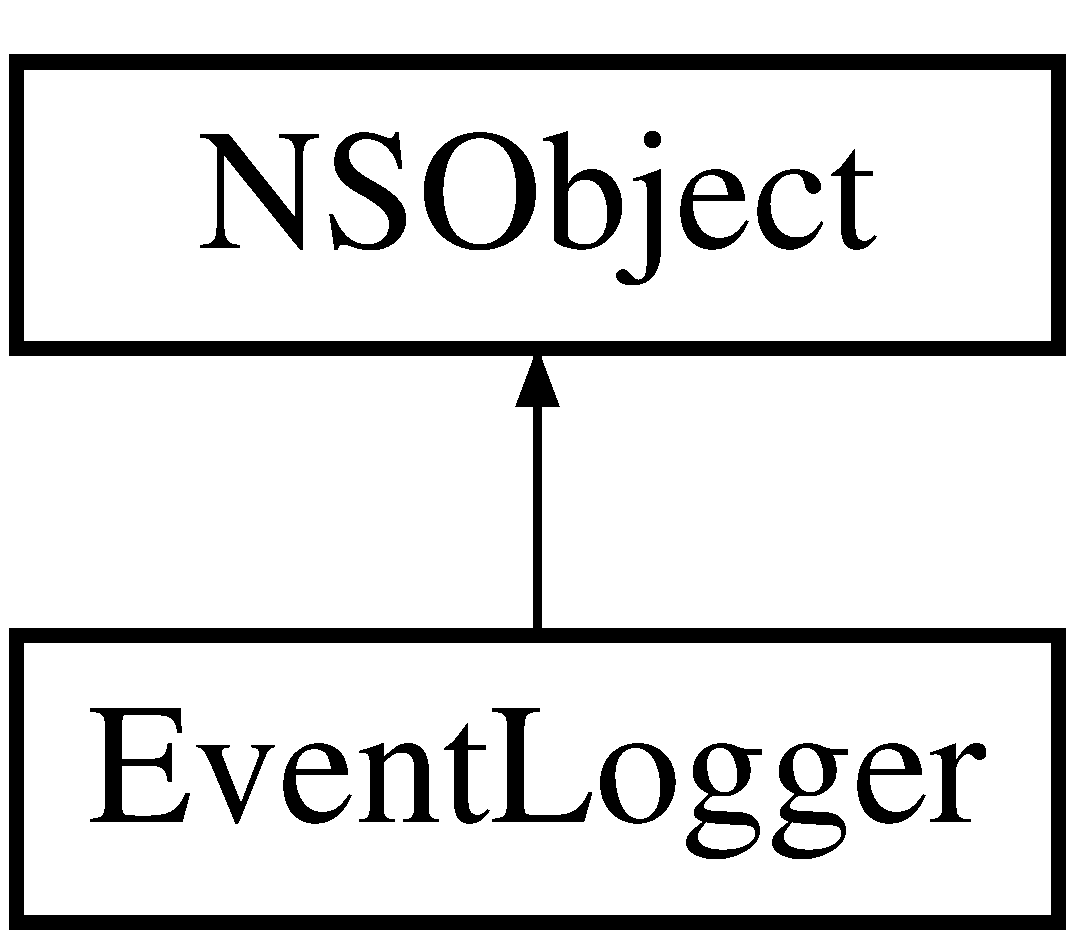
\includegraphics[height=2.000000cm]{interface_event_logger}
\end{center}
\end{figure}
\subsection*{Instance Methods}
\begin{DoxyCompactItemize}
\item 
(void) -\/ \hyperlink{interface_event_logger_aa085061d6f02d4b8b40c8b347c676f9f}{add\-Event\-:}
\item 
(N\-S\-Mutable\-Array $\ast$) -\/ \hyperlink{interface_event_logger_ac66e3dc819bc1cf129a2141875b440a3}{create\-Events\-Output}
\item 
(void) -\/ \hyperlink{interface_event_logger_a0ad12aea4a582b9d7393847f90718307}{clear\-Events\-List\-:}
\item 
\hypertarget{interface_event_logger_a60120e85b3b04e0212654fd51bc1a679}{(void) -\/ \hyperlink{interface_event_logger_a60120e85b3b04e0212654fd51bc1a679}{populate\-Event\-Key}}\label{interface_event_logger_a60120e85b3b04e0212654fd51bc1a679}

\begin{DoxyCompactList}\small\item\em Maps the event description to the corresponding description id and adds it to the events key array. \end{DoxyCompactList}\end{DoxyCompactItemize}
\subsection*{Class Methods}
\begin{DoxyCompactItemize}
\item 
(\hyperlink{interface_event_logger}{Event\-Logger} $\ast$) + \hyperlink{interface_event_logger_a6343b40276111dd1d7275bbde3a3e508}{shared\-Event\-Logger}
\end{DoxyCompactItemize}
\subsection*{Properties}
\begin{DoxyCompactItemize}
\item 
\hypertarget{interface_event_logger_a67a1a529ac51538c28ff99617238ebcc}{N\-S\-Mutable\-Array $\ast$ \hyperlink{interface_event_logger_a67a1a529ac51538c28ff99617238ebcc}{events}}\label{interface_event_logger_a67a1a529ac51538c28ff99617238ebcc}

\begin{DoxyCompactList}\small\item\em An array containing all of the events that occur in the app. \end{DoxyCompactList}\item 
\hypertarget{interface_event_logger_a85a7cbe7f3811f03518390b615822105}{N\-S\-Mutable\-Dictionary $\ast$ \hyperlink{interface_event_logger_a85a7cbe7f3811f03518390b615822105}{events\-Key}}\label{interface_event_logger_a85a7cbe7f3811f03518390b615822105}

\begin{DoxyCompactList}\small\item\em An array containing the mapping of event ids to their description. \end{DoxyCompactList}\end{DoxyCompactItemize}


\subsection{Detailed Description}
A class used to keep a record of all of the events the user makes during a modeling session. 

\subsection{Method Documentation}
\hypertarget{interface_event_logger_aa085061d6f02d4b8b40c8b347c676f9f}{\index{Event\-Logger@{Event\-Logger}!add\-Event\-:@{add\-Event\-:}}
\index{add\-Event\-:@{add\-Event\-:}!EventLogger@{Event\-Logger}}
\subsubsection[{add\-Event\-:}]{\setlength{\rightskip}{0pt plus 5cm}-\/ (void) add\-Event\-: 
\begin{DoxyParamCaption}
\item[{({\bf Event}$\ast$)}]{new\-Event}
\end{DoxyParamCaption}
}}\label{interface_event_logger_aa085061d6f02d4b8b40c8b347c676f9f}
Will add a record in the event log with the time stamp and the event that occurred. 
\begin{DoxyParams}{Parameters}
{\em new\-Event} & an instance of an \hyperlink{interface_event}{Event} containing the details of the event that should be added. \\
\hline
\end{DoxyParams}
\hypertarget{interface_event_logger_a0ad12aea4a582b9d7393847f90718307}{\index{Event\-Logger@{Event\-Logger}!clear\-Events\-List\-:@{clear\-Events\-List\-:}}
\index{clear\-Events\-List\-:@{clear\-Events\-List\-:}!EventLogger@{Event\-Logger}}
\subsubsection[{clear\-Events\-List\-:}]{\setlength{\rightskip}{0pt plus 5cm}-\/ (void) clear\-Events\-List\-: 
\begin{DoxyParamCaption}
\item[{(int)}]{num}
\end{DoxyParamCaption}
}}\label{interface_event_logger_a0ad12aea4a582b9d7393847f90718307}
Removes all of the events in the list. 
\begin{DoxyParams}{Parameters}
{\em num} & the last event that was saved to the database. \\
\hline
\end{DoxyParams}
\hypertarget{interface_event_logger_ac66e3dc819bc1cf129a2141875b440a3}{\index{Event\-Logger@{Event\-Logger}!create\-Events\-Output@{create\-Events\-Output}}
\index{create\-Events\-Output@{create\-Events\-Output}!EventLogger@{Event\-Logger}}
\subsubsection[{create\-Events\-Output}]{\setlength{\rightskip}{0pt plus 5cm}-\/ (N\-S\-Mutable\-Array $\ast$) create\-Events\-Output 
\begin{DoxyParamCaption}
{}
\end{DoxyParamCaption}
}}\label{interface_event_logger_ac66e3dc819bc1cf129a2141875b440a3}
Constructs the file of events for the analysis. \begin{DoxyReturn}{Returns}
an array of events with formatted output. 
\end{DoxyReturn}
\hypertarget{interface_event_logger_a6343b40276111dd1d7275bbde3a3e508}{\index{Event\-Logger@{Event\-Logger}!shared\-Event\-Logger@{shared\-Event\-Logger}}
\index{shared\-Event\-Logger@{shared\-Event\-Logger}!EventLogger@{Event\-Logger}}
\subsubsection[{shared\-Event\-Logger}]{\setlength{\rightskip}{0pt plus 5cm}+ ({\bf Event\-Logger} $\ast$) shared\-Event\-Logger 
\begin{DoxyParamCaption}
{}
\end{DoxyParamCaption}
}}\label{interface_event_logger_a6343b40276111dd1d7275bbde3a3e508}
Forces the \hyperlink{interface_event_logger}{Event\-Logger} to be a singleton class. \begin{DoxyReturn}{Returns}
a pointer to the single instance of the event logger. 
\end{DoxyReturn}


The documentation for this class was generated from the following files\-:\begin{DoxyCompactItemize}
\item 
Group\-Modeling\-App/Event\-Logger.\-h\item 
Group\-Modeling\-App/Event\-Logger.\-m\end{DoxyCompactItemize}

\hypertarget{interface_file_i_o}{\section{File\-I\-O Class Reference}
\label{interface_file_i_o}\index{File\-I\-O@{File\-I\-O}}
}


A class that handles the parsing of mdl files to import into the application. Also is responsible for exporting the model back into a Vensim file for saving state and for use in Vensim again.  




{\ttfamily \#import $<$File\-I\-O.\-h$>$}

Inheritance diagram for File\-I\-O\-:\begin{figure}[H]
\begin{center}
\leavevmode
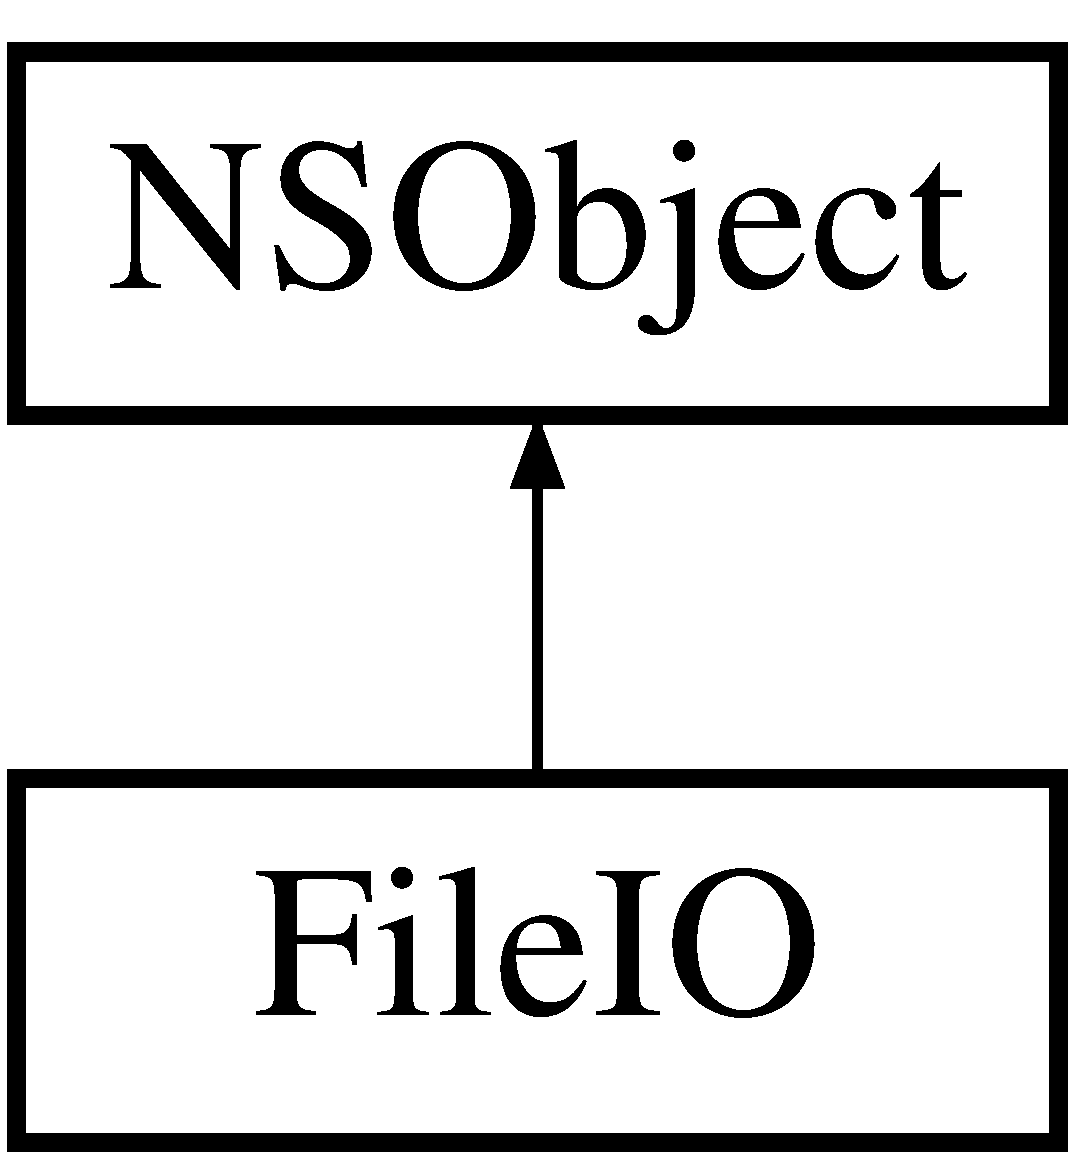
\includegraphics[height=2.000000cm]{interface_file_i_o}
\end{center}
\end{figure}
\subsection*{Instance Methods}
\begin{DoxyCompactItemize}
\item 
(void) -\/ \hyperlink{interface_file_i_o_a2bb3d58ae1f0fac924e831a424e1365b}{import\-Model\-:}
\item 
(N\-S\-String $\ast$) -\/ \hyperlink{interface_file_i_o_a521b8da51a857f38be6622a220cf70c5}{open\-File}
\item 
(N\-S\-U\-R\-L $\ast$) -\/ \hyperlink{interface_file_i_o_ae00d68df671c5290f0e6774adf469f49}{export\-Model}
\item 
\hypertarget{interface_file_i_o_ab012ca0b3749e8e0fb26a09a92d28d02}{(void) -\/ \hyperlink{interface_file_i_o_ab012ca0b3749e8e0fb26a09a92d28d02}{export\-Event\-Logging}}\label{interface_file_i_o_ab012ca0b3749e8e0fb26a09a92d28d02}

\begin{DoxyCompactList}\small\item\em Will export the model event logging data and write it to a file event\-Logging.\-txt. \end{DoxyCompactList}\item 
(N\-S\-Number $\ast$) -\/ \hyperlink{interface_file_i_o_a628a9ac631ce93a2e49ac8155b62eaf1}{get\-File\-I\-D}
\item 
(N\-S\-Number $\ast$) -\/ \hyperlink{interface_file_i_o_a305324f84521a6c2966a744c620c6009}{get\-Next\-Available\-File\-I\-D}
\item 
(void) -\/ \hyperlink{interface_file_i_o_a00a3fe9bd4e7c407327987606c18028a}{process\-Component\-:loop\-Name\-:}
\item 
\hypertarget{interface_file_i_o_a0282f6418e27f223af8dc89cc5142d31}{(void) -\/ \hyperlink{interface_file_i_o_a0282f6418e27f223af8dc89cc5142d31}{update\-Causal\-Link\-Connections}}\label{interface_file_i_o_a0282f6418e27f223af8dc89cc5142d31}

\begin{DoxyCompactList}\small\item\em Once the file has been read in completely we can finish processing the data. The causal link parent and child objects upon import point to a string id of the parent and child, instead we would like the parent and child to point to the instance of those Variables. Likewise, each variable would like to keep track of which Causal\-Links are indegree and outdegree. \end{DoxyCompactList}\end{DoxyCompactItemize}
\subsection*{Class Methods}
\begin{DoxyCompactItemize}
\item 
(\hyperlink{interface_file_i_o}{File\-I\-O} $\ast$) + \hyperlink{interface_file_i_o_a010550b3de2e660a2a14d4dce2990078}{shared\-File\-I\-O}
\item 
(N\-S\-Data $\ast$) + \hyperlink{interface_file_i_o_ac570de2e8f37bc126a9f9536f34bc09d}{sha1\-:}
\item 
(N\-S\-String $\ast$) + \hyperlink{interface_file_i_o_a3e844772cd8f89ba85d4bd369a093fd8}{base64for\-Data\-:}
\end{DoxyCompactItemize}


\subsection{Detailed Description}
A class that handles the parsing of mdl files to import into the application. Also is responsible for exporting the model back into a Vensim file for saving state and for use in Vensim again. 

\subsection{Method Documentation}
\hypertarget{interface_file_i_o_a3e844772cd8f89ba85d4bd369a093fd8}{\index{File\-I\-O@{File\-I\-O}!base64for\-Data\-:@{base64for\-Data\-:}}
\index{base64for\-Data\-:@{base64for\-Data\-:}!FileIO@{File\-I\-O}}
\subsubsection[{base64for\-Data\-:}]{\setlength{\rightskip}{0pt plus 5cm}+ (N\-S\-String $\ast$) base64for\-Data\-: 
\begin{DoxyParamCaption}
\item[{(N\-S\-Data$\ast$)}]{the\-Data}
\end{DoxyParamCaption}
}}\label{interface_file_i_o_a3e844772cd8f89ba85d4bd369a093fd8}
Converts the hashed dat to a base64 string for comparison with what is stored in the database. 
\begin{DoxyParams}{Parameters}
{\em the\-Data} & the hash value to be converted. \\
\hline
\end{DoxyParams}
\begin{DoxyReturn}{Returns}
the converted nsdata to base64 string 
\end{DoxyReturn}
\hypertarget{interface_file_i_o_ae00d68df671c5290f0e6774adf469f49}{\index{File\-I\-O@{File\-I\-O}!export\-Model@{export\-Model}}
\index{export\-Model@{export\-Model}!FileIO@{File\-I\-O}}
\subsubsection[{export\-Model}]{\setlength{\rightskip}{0pt plus 5cm}-\/ (N\-S\-U\-R\-L $\ast$) export\-Model 
\begin{DoxyParamCaption}
{}
\end{DoxyParamCaption}
}}\label{interface_file_i_o_ae00d68df671c5290f0e6774adf469f49}
Will export the model and write it to a file output.\-mdl. \begin{DoxyReturn}{Returns}
the url location of the file. 
\end{DoxyReturn}
Add the current max I\-D, used for tracking events. Stored as -\/\#\#. \hypertarget{interface_file_i_o_a628a9ac631ce93a2e49ac8155b62eaf1}{\index{File\-I\-O@{File\-I\-O}!get\-File\-I\-D@{get\-File\-I\-D}}
\index{get\-File\-I\-D@{get\-File\-I\-D}!FileIO@{File\-I\-O}}
\subsubsection[{get\-File\-I\-D}]{\setlength{\rightskip}{0pt plus 5cm}-\/ (N\-S\-Number $\ast$) get\-File\-I\-D 
\begin{DoxyParamCaption}
{}
\end{DoxyParamCaption}
}}\label{interface_file_i_o_a628a9ac631ce93a2e49ac8155b62eaf1}
Get the parent file global idenitifer (gid) so we can keep track of when a specific user modifies the same file or any derivative of the original file. The gid will be unique per user + parent file combination. \begin{DoxyReturn}{Returns}
a gid value for this eventlog record. 
\end{DoxyReturn}
\hypertarget{interface_file_i_o_a305324f84521a6c2966a744c620c6009}{\index{File\-I\-O@{File\-I\-O}!get\-Next\-Available\-File\-I\-D@{get\-Next\-Available\-File\-I\-D}}
\index{get\-Next\-Available\-File\-I\-D@{get\-Next\-Available\-File\-I\-D}!FileIO@{File\-I\-O}}
\subsubsection[{get\-Next\-Available\-File\-I\-D}]{\setlength{\rightskip}{0pt plus 5cm}-\/ (N\-S\-Number $\ast$) get\-Next\-Available\-File\-I\-D 
\begin{DoxyParamCaption}
{}
\end{DoxyParamCaption}
}}\label{interface_file_i_o_a305324f84521a6c2966a744c620c6009}
If a new file has been created, or a user has not edited an existing file before, we will need to create a new gid for this user/file combination. \begin{DoxyReturn}{Returns}
the next available file gid in the database. 
\end{DoxyReturn}
\hypertarget{interface_file_i_o_a2bb3d58ae1f0fac924e831a424e1365b}{\index{File\-I\-O@{File\-I\-O}!import\-Model\-:@{import\-Model\-:}}
\index{import\-Model\-:@{import\-Model\-:}!FileIO@{File\-I\-O}}
\subsubsection[{import\-Model\-:}]{\setlength{\rightskip}{0pt plus 5cm}-\/ (void) import\-Model\-: 
\begin{DoxyParamCaption}
\item[{(N\-S\-Array$\ast$)}]{lines}
\end{DoxyParamCaption}
}}\label{interface_file_i_o_a2bb3d58ae1f0fac924e831a424e1365b}
Opens a Vensim mdl file and parses through it to populate the model. Will update the \hyperlink{interface_model}{Model} object with its simulation control parameters, default model parameters, and all components including any \hyperlink{interface_variable}{Variable}, \hyperlink{interface_causal_link}{Causal\-Link}, and \hyperlink{interface_loop}{Loop}. \begin{DoxyRefDesc}{Todo}
\item[\hyperlink{todo__todo000003}{Todo}]The name of the loop being on the next line kind of a pain \end{DoxyRefDesc}
\hypertarget{interface_file_i_o_a521b8da51a857f38be6622a220cf70c5}{\index{File\-I\-O@{File\-I\-O}!open\-File@{open\-File}}
\index{open\-File@{open\-File}!FileIO@{File\-I\-O}}
\subsubsection[{open\-File}]{\setlength{\rightskip}{0pt plus 5cm}-\/ (N\-S\-String $\ast$) open\-File 
\begin{DoxyParamCaption}
{}
\end{DoxyParamCaption}
}}\label{interface_file_i_o_a521b8da51a857f38be6622a220cf70c5}
Will open the selected Vensim file to import and use. \begin{DoxyNote}{Note}
this is only used when wanting to test in the simulator. 
\end{DoxyNote}
\begin{DoxyReturn}{Returns}
a string contraining the entire file 
\end{DoxyReturn}
\hypertarget{interface_file_i_o_a00a3fe9bd4e7c407327987606c18028a}{\index{File\-I\-O@{File\-I\-O}!process\-Component\-:loop\-Name\-:@{process\-Component\-:loop\-Name\-:}}
\index{process\-Component\-:loop\-Name\-:@{process\-Component\-:loop\-Name\-:}!FileIO@{File\-I\-O}}
\subsubsection[{process\-Component\-:loop\-Name\-:}]{\setlength{\rightskip}{0pt plus 5cm}-\/ (void) process\-Component\-: 
\begin{DoxyParamCaption}
\item[{(N\-S\-String$\ast$)}]{string}
\item[{loopName:(N\-S\-String$\ast$)}]{loop\-Name}
\end{DoxyParamCaption}
}}\label{interface_file_i_o_a00a3fe9bd4e7c407327987606c18028a}
Will create a new component of type \hyperlink{interface_causal_link}{Causal\-Link}, \hyperlink{interface_variable}{Variable}, or \hyperlink{interface_loop}{Loop} and add it to the model. 
\begin{DoxyParams}{Parameters}
{\em string} & the input string from the Vensim mdl file that provides specification for the component. \\
\hline
{\em loop\-Name} & the provided name for a loop. This will be ignored for causal links and variables. \\
\hline
\end{DoxyParams}
\hypertarget{interface_file_i_o_ac570de2e8f37bc126a9f9536f34bc09d}{\index{File\-I\-O@{File\-I\-O}!sha1\-:@{sha1\-:}}
\index{sha1\-:@{sha1\-:}!FileIO@{File\-I\-O}}
\subsubsection[{sha1\-:}]{\setlength{\rightskip}{0pt plus 5cm}+ (N\-S\-Data $\ast$) sha1\-: 
\begin{DoxyParamCaption}
\item[{(N\-S\-Data $\ast$)}]{data}
\end{DoxyParamCaption}
}}\label{interface_file_i_o_ac570de2e8f37bc126a9f9536f34bc09d}
Will compute a sha1 hash function on some data. 
\begin{DoxyParams}{Parameters}
{\em data} & the data to be hashed. \\
\hline
{\em a} & sha1 hash of data. \\
\hline
\end{DoxyParams}
\hypertarget{interface_file_i_o_a010550b3de2e660a2a14d4dce2990078}{\index{File\-I\-O@{File\-I\-O}!shared\-File\-I\-O@{shared\-File\-I\-O}}
\index{shared\-File\-I\-O@{shared\-File\-I\-O}!FileIO@{File\-I\-O}}
\subsubsection[{shared\-File\-I\-O}]{\setlength{\rightskip}{0pt plus 5cm}+ ({\bf File\-I\-O} $\ast$) shared\-File\-I\-O 
\begin{DoxyParamCaption}
{}
\end{DoxyParamCaption}
}}\label{interface_file_i_o_a010550b3de2e660a2a14d4dce2990078}
Forces the \hyperlink{interface_model}{Model} to be a singleton class. \begin{DoxyReturn}{Returns}
a pointer to the single instance of the model. 
\end{DoxyReturn}


The documentation for this class was generated from the following files\-:\begin{DoxyCompactItemize}
\item 
Group\-Modeling\-App/File\-I\-O.\-h\item 
Group\-Modeling\-App/File\-I\-O.\-m\end{DoxyCompactItemize}

\hypertarget{interface_help_section_view_controller}{\section{Help\-Section\-View\-Controller Class Reference}
\label{interface_help_section_view_controller}\index{Help\-Section\-View\-Controller@{Help\-Section\-View\-Controller}}
}


A Table view controller used to handle the help section.  




{\ttfamily \#import $<$Help\-Section\-View\-Controller.\-h$>$}

Inheritance diagram for Help\-Section\-View\-Controller\-:\begin{figure}[H]
\begin{center}
\leavevmode
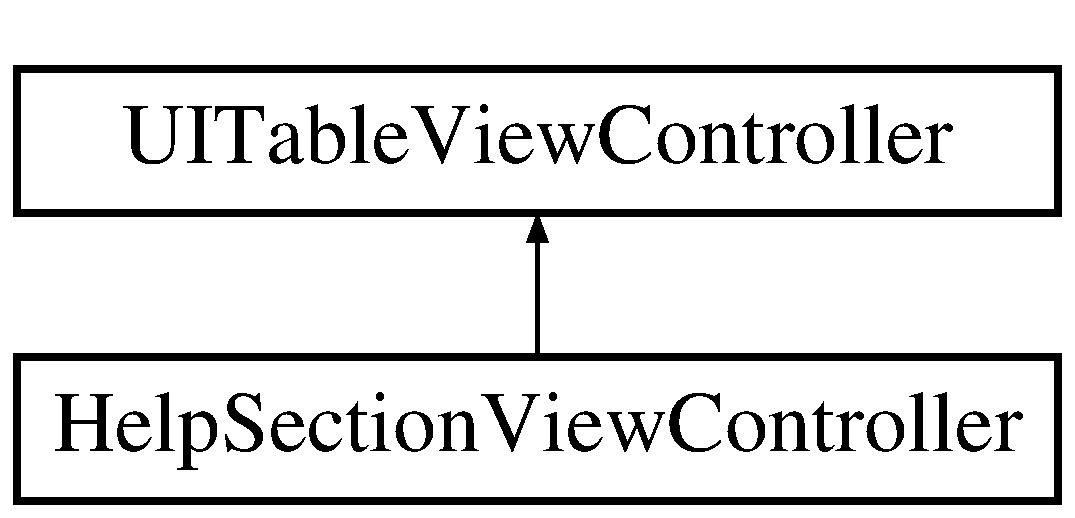
\includegraphics[height=2.000000cm]{interface_help_section_view_controller}
\end{center}
\end{figure}
\subsection*{Instance Methods}
\begin{DoxyCompactItemize}
\item 
(\hyperlink{interface_m_f_side_menu_container_view_controller}{M\-F\-Side\-Menu\-Container\-View\-Controller} $\ast$) -\/ \hyperlink{interface_help_section_view_controller_ad9f497773e1c2f5e420929a60f3bf7df}{menu\-Container\-View\-Controller}
\item 
\hypertarget{interface_help_section_view_controller_a9644bcb73520daa217ad0709b0e6bd64}{(void) -\/ \hyperlink{interface_help_section_view_controller_a9644bcb73520daa217ad0709b0e6bd64}{setup\-Menu\-Bar\-Button\-Items}}\label{interface_help_section_view_controller_a9644bcb73520daa217ad0709b0e6bd64}

\begin{DoxyCompactList}\small\item\em Sets up the menu bar of the view controller. \end{DoxyCompactList}\item 
(U\-I\-Bar\-Button\-Item $\ast$) -\/ \hyperlink{interface_help_section_view_controller_afb11718c8a0c6f7abd85dfbc7adb1cd1}{left\-Menu\-Bar\-Button\-Item}
\item 
(void) -\/ \hyperlink{interface_help_section_view_controller_a738b842dc5261f08da93880f0b006b55}{left\-Side\-Menu\-Button\-Pressed\-:}
\end{DoxyCompactItemize}


\subsection{Detailed Description}
A Table view controller used to handle the help section. 

\subsection{Method Documentation}
\hypertarget{interface_help_section_view_controller_afb11718c8a0c6f7abd85dfbc7adb1cd1}{\index{Help\-Section\-View\-Controller@{Help\-Section\-View\-Controller}!left\-Menu\-Bar\-Button\-Item@{left\-Menu\-Bar\-Button\-Item}}
\index{left\-Menu\-Bar\-Button\-Item@{left\-Menu\-Bar\-Button\-Item}!HelpSectionViewController@{Help\-Section\-View\-Controller}}
\subsubsection[{left\-Menu\-Bar\-Button\-Item}]{\setlength{\rightskip}{0pt plus 5cm}-\/ (U\-I\-Bar\-Button\-Item $\ast$) left\-Menu\-Bar\-Button\-Item 
\begin{DoxyParamCaption}
{}
\end{DoxyParamCaption}
}}\label{interface_help_section_view_controller_afb11718c8a0c6f7abd85dfbc7adb1cd1}
Creates the left menu bar button item. This item will be responsible for opening the menu. \begin{DoxyReturn}{Returns}
the left menu bar button item. 
\end{DoxyReturn}
\hypertarget{interface_help_section_view_controller_a738b842dc5261f08da93880f0b006b55}{\index{Help\-Section\-View\-Controller@{Help\-Section\-View\-Controller}!left\-Side\-Menu\-Button\-Pressed\-:@{left\-Side\-Menu\-Button\-Pressed\-:}}
\index{left\-Side\-Menu\-Button\-Pressed\-:@{left\-Side\-Menu\-Button\-Pressed\-:}!HelpSectionViewController@{Help\-Section\-View\-Controller}}
\subsubsection[{left\-Side\-Menu\-Button\-Pressed\-:}]{\setlength{\rightskip}{0pt plus 5cm}-\/ (void) left\-Side\-Menu\-Button\-Pressed\-: 
\begin{DoxyParamCaption}
\item[{(id)}]{sender}
\end{DoxyParamCaption}
}}\label{interface_help_section_view_controller_a738b842dc5261f08da93880f0b006b55}
Callback for when the left menu button is pressed. 
\begin{DoxyParams}{Parameters}
{\em sender} & the id of the sender object. \\
\hline
\end{DoxyParams}
\hypertarget{interface_help_section_view_controller_ad9f497773e1c2f5e420929a60f3bf7df}{\index{Help\-Section\-View\-Controller@{Help\-Section\-View\-Controller}!menu\-Container\-View\-Controller@{menu\-Container\-View\-Controller}}
\index{menu\-Container\-View\-Controller@{menu\-Container\-View\-Controller}!HelpSectionViewController@{Help\-Section\-View\-Controller}}
\subsubsection[{menu\-Container\-View\-Controller}]{\setlength{\rightskip}{0pt plus 5cm}-\/ ({\bf M\-F\-Side\-Menu\-Container\-View\-Controller} $\ast$) menu\-Container\-View\-Controller 
\begin{DoxyParamCaption}
{}
\end{DoxyParamCaption}
}}\label{interface_help_section_view_controller_ad9f497773e1c2f5e420929a60f3bf7df}
Gets the menu container view controller. \begin{DoxyReturn}{Returns}
the menu container view controller. 
\end{DoxyReturn}


The documentation for this class was generated from the following files\-:\begin{DoxyCompactItemize}
\item 
Group\-Modeling\-App/Help\-Section\-View\-Controller.\-h\item 
Group\-Modeling\-App/Help\-Section\-View\-Controller.\-m\end{DoxyCompactItemize}

\hypertarget{category_help_section_view_controller_07_08}{\section{Help\-Section\-View\-Controller() Category Reference}
\label{category_help_section_view_controller_07_08}\index{Help\-Section\-View\-Controller()@{Help\-Section\-View\-Controller()}}
}


The documentation for this category was generated from the following file\-:\begin{DoxyCompactItemize}
\item 
Group\-Modeling\-App/Help\-Section\-View\-Controller.\-m\end{DoxyCompactItemize}

\hypertarget{interface_loop}{\section{Loop Class Reference}
\label{interface_loop}\index{Loop@{Loop}}
}


A subclass of \hyperlink{interface_component}{Component} containing the data related to a feedback loop of a causal loop diagram. ex. In a diagram on K-\/12 school attendance, a feedback loop would occur where as \char`\"{}\-Students Desire to Go to School\char`\"{} increases so does their \char`\"{}\-Mean daily attendance rate\char`\"{} and as their \char`\"{}\-Mean Daily attendance rate\char`\"{} increases so does a \char`\"{}\-Students Desire to Go to School\char`\"{}.  




{\ttfamily \#import $<$Loop.\-h$>$}

Inheritance diagram for Loop\-:\begin{figure}[H]
\begin{center}
\leavevmode
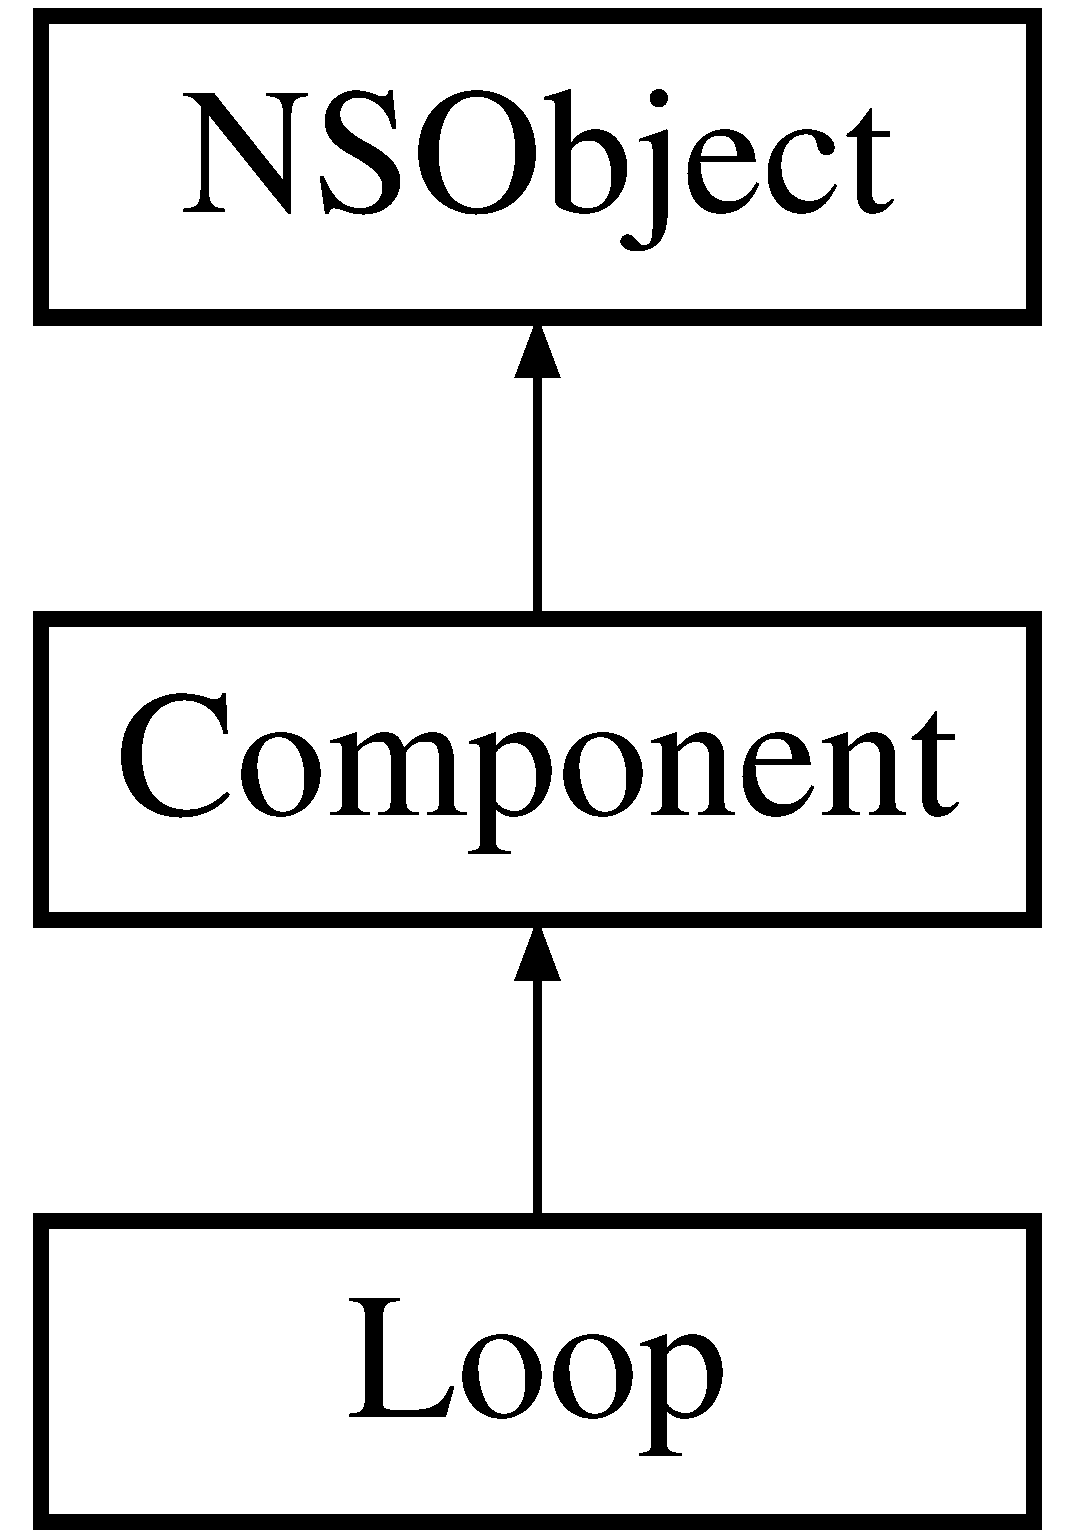
\includegraphics[height=3.000000cm]{interface_loop}
\end{center}
\end{figure}
\subsection*{Instance Methods}
\begin{DoxyCompactItemize}
\item 
(id) -\/ \hyperlink{interface_loop_ad35655514796f99b2f95f9d97ee9cbc1}{init\-:var\-Name\-:}
\item 
(id) -\/ \hyperlink{interface_loop_a9755af4c66523c228c80713cab6396fe}{init\-With\-Location\-:}
\item 
(N\-S\-String $\ast$) -\/ \hyperlink{interface_loop_a404a48142c96cacac68633e2d2c00701}{create\-Loop\-Output\-String}
\end{DoxyCompactItemize}
\subsection*{Properties}
\begin{DoxyCompactItemize}
\item 
\hypertarget{interface_loop_a0e3597199260a059ec632e5d54adb06e}{int \hyperlink{interface_loop_a0e3597199260a059ec632e5d54adb06e}{text\-Position}}\label{interface_loop_a0e3597199260a059ec632e5d54adb06e}

\begin{DoxyCompactList}\small\item\em Where the text holding the feedback loop name is located in relation to the feedback loop object. \end{DoxyCompactList}\item 
\hypertarget{interface_loop_a73b1ecad68943855563486ea8848e95f}{\hyperlink{interface_loop_view}{Loop\-View} $\ast$ \hyperlink{interface_loop_a73b1ecad68943855563486ea8848e95f}{view}}\label{interface_loop_a73b1ecad68943855563486ea8848e95f}

\begin{DoxyCompactList}\small\item\em The U\-I\-View that will contain the graphical representation of the loop. \end{DoxyCompactList}\end{DoxyCompactItemize}
\subsection*{Additional Inherited Members}


\subsection{Detailed Description}
A subclass of \hyperlink{interface_component}{Component} containing the data related to a feedback loop of a causal loop diagram. ex. In a diagram on K-\/12 school attendance, a feedback loop would occur where as \char`\"{}\-Students Desire to Go to School\char`\"{} increases so does their \char`\"{}\-Mean daily attendance rate\char`\"{} and as their \char`\"{}\-Mean Daily attendance rate\char`\"{} increases so does a \char`\"{}\-Students Desire to Go to School\char`\"{}. 

\subsection{Method Documentation}
\hypertarget{interface_loop_a404a48142c96cacac68633e2d2c00701}{\index{Loop@{Loop}!create\-Loop\-Output\-String@{create\-Loop\-Output\-String}}
\index{create\-Loop\-Output\-String@{create\-Loop\-Output\-String}!Loop@{Loop}}
\subsubsection[{create\-Loop\-Output\-String}]{\setlength{\rightskip}{0pt plus 5cm}-\/ (N\-S\-String $\ast$) create\-Loop\-Output\-String 
\begin{DoxyParamCaption}
{}
\end{DoxyParamCaption}
}}\label{interface_loop_a404a48142c96cacac68633e2d2c00701}
Constructs the output string for a \hyperlink{interface_loop}{Loop}. The string is constructed to be readable by Vensim. Follows the string pattern\-: \mbox{[}Object Type\mbox{]},\mbox{[}Object id\mbox{]},0,\mbox{[}X Location\mbox{]},\mbox{[}Y Location\mbox{]},20,20,\mbox{[}Symbol\mbox{]},7,0,0,\mbox{[}Text Position\mbox{]},0,0,0,\mbox{[}Shape color\mbox{]},\mbox{[}Background Color\mbox{]} \mbox{[}Comment\mbox{]} \begin{DoxyReturn}{Returns}
the string of data for the variable. 
\end{DoxyReturn}
\hypertarget{interface_loop_ad35655514796f99b2f95f9d97ee9cbc1}{\index{Loop@{Loop}!init\-:var\-Name\-:@{init\-:var\-Name\-:}}
\index{init\-:var\-Name\-:@{init\-:var\-Name\-:}!Loop@{Loop}}
\subsubsection[{init\-:var\-Name\-:}]{\setlength{\rightskip}{0pt plus 5cm}-\/ (id) init\-: 
\begin{DoxyParamCaption}
\item[{(N\-S\-Array$\ast$)}]{data}
\item[{varName:(N\-S\-String$\ast$)}]{my\-Name}
\end{DoxyParamCaption}
}}\label{interface_loop_ad35655514796f99b2f95f9d97ee9cbc1}
Initializes the \hyperlink{interface_loop}{Loop} when you are reading from an mdl file. 
\begin{DoxyParams}{Parameters}
{\em data} & an array of strings containing all of the data for the feedback loop from a Vensim mdl file. \\
\hline
{\em my\-Name} & the name associated with the feedback loop. Unlike Variables and Causal\-Links, \hyperlink{interface_loop}{Loop} names are located on a different line in the Vensim mdl file from the rest of the loop attributes. \\
\hline
\end{DoxyParams}
\begin{DoxyReturn}{Returns}
a pointer to the newly created \hyperlink{interface_loop}{Loop}. 
\end{DoxyReturn}
\hypertarget{interface_loop_a9755af4c66523c228c80713cab6396fe}{\index{Loop@{Loop}!init\-With\-Location\-:@{init\-With\-Location\-:}}
\index{init\-With\-Location\-:@{init\-With\-Location\-:}!Loop@{Loop}}
\subsubsection[{init\-With\-Location\-:}]{\setlength{\rightskip}{0pt plus 5cm}-\/ (id) init\-With\-Location\-: 
\begin{DoxyParamCaption}
\item[{(C\-G\-Point)}]{location}
\end{DoxyParamCaption}
}}\label{interface_loop_a9755af4c66523c228c80713cab6396fe}
Initizlizes the \hyperlink{interface_loop}{Loop} when you are adding a brand new variable. 
\begin{DoxyParams}{Parameters}
{\em location} & the location of the new object in the frame. \\
\hline
\end{DoxyParams}
\begin{DoxyReturn}{Returns}
a pointer to the newly created \hyperlink{interface_loop}{Loop}. 
\end{DoxyReturn}


The documentation for this class was generated from the following files\-:\begin{DoxyCompactItemize}
\item 
Group\-Modeling\-App/Loop.\-h\item 
Group\-Modeling\-App/Loop.\-m\end{DoxyCompactItemize}

\hypertarget{interface_loop_edit_menu_view}{\section{Loop\-Edit\-Menu\-View Class Reference}
\label{interface_loop_edit_menu_view}\index{Loop\-Edit\-Menu\-View@{Loop\-Edit\-Menu\-View}}
}


The view that will contain the edit menu for Loops.  




{\ttfamily \#import $<$Loop\-Edit\-Menu\-View.\-h$>$}

Inheritance diagram for Loop\-Edit\-Menu\-View\-:\begin{figure}[H]
\begin{center}
\leavevmode
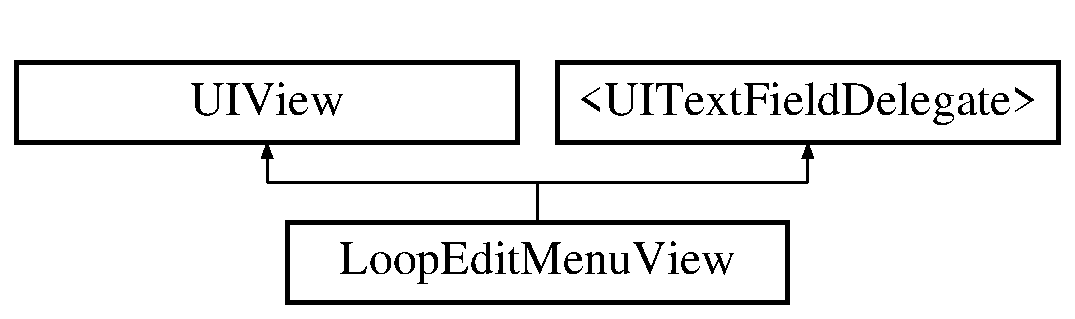
\includegraphics[height=2.000000cm]{interface_loop_edit_menu_view}
\end{center}
\end{figure}
\subsection*{Instance Methods}
\begin{DoxyCompactItemize}
\item 
(id) -\/ \hyperlink{interface_loop_edit_menu_view_ad1475d40e606d4f009f89321944e3678}{init\-With\-Frame\-:view\-:}
\item 
\hypertarget{interface_loop_edit_menu_view_ae0f43dc61fe8f377acde5d5c252b6c0e}{(void) -\/ \hyperlink{interface_loop_edit_menu_view_ae0f43dc61fe8f377acde5d5c252b6c0e}{update\-Loop}}\label{interface_loop_edit_menu_view_ae0f43dc61fe8f377acde5d5c252b6c0e}

\begin{DoxyCompactList}\small\item\em This method will be called when the save button is called to save the attributes. \end{DoxyCompactList}\item 
\hypertarget{interface_loop_edit_menu_view_a8395f57f6403f4f8775c1062aca14bc6}{(void) -\/ \hyperlink{interface_loop_edit_menu_view_a8395f57f6403f4f8775c1062aca14bc6}{symbol\-Control\-Change}}\label{interface_loop_edit_menu_view_a8395f57f6403f4f8775c1062aca14bc6}

\begin{DoxyCompactList}\small\item\em Notifies the logger when a new option from the symbol segmented control has been changed. \end{DoxyCompactList}\item 
(void) -\/ \hyperlink{interface_loop_edit_menu_view_ac9394b979597f8df8e15f5abc1cc7a2e}{text\-Field\-Did\-Begin\-Editing\-:}
\item 
(void) -\/ \hyperlink{interface_loop_edit_menu_view_aa7337263d1e997c99cdc506fc61dcea3}{text\-Field\-Did\-End\-Editing\-:}
\item 
(B\-O\-O\-L) -\/ \hyperlink{interface_loop_edit_menu_view_a1a8ec9c257f3a894dc9b3389477f55e9}{text\-Field\-Should\-Return\-:}
\end{DoxyCompactItemize}
\subsection*{Properties}
\begin{DoxyCompactItemize}
\item 
\hypertarget{interface_loop_edit_menu_view_af91fc4ee7ce5ce8ac3b0f00e38824b04}{U\-I\-Label $\ast$ \hyperlink{interface_loop_edit_menu_view_af91fc4ee7ce5ce8ac3b0f00e38824b04}{name\-Label}}\label{interface_loop_edit_menu_view_af91fc4ee7ce5ce8ac3b0f00e38824b04}

\begin{DoxyCompactList}\small\item\em The label that represents what name\-Text\-Field represents. \end{DoxyCompactList}\item 
\hypertarget{interface_loop_edit_menu_view_a5cbc9eaf5c10f7b61fa933746ae0bb6e}{U\-I\-Text\-Field $\ast$ \hyperlink{interface_loop_edit_menu_view_a5cbc9eaf5c10f7b61fa933746ae0bb6e}{name\-Text\-Field}}\label{interface_loop_edit_menu_view_a5cbc9eaf5c10f7b61fa933746ae0bb6e}

\begin{DoxyCompactList}\small\item\em The text field that contains the name of the object. \end{DoxyCompactList}\item 
\hypertarget{interface_loop_edit_menu_view_a6fdbff14250b254546c94f76fc96d7d6}{\hyperlink{interface_loop_view}{Loop\-View} $\ast$ \hyperlink{interface_loop_edit_menu_view_a6fdbff14250b254546c94f76fc96d7d6}{object\-View}}\label{interface_loop_edit_menu_view_a6fdbff14250b254546c94f76fc96d7d6}

\begin{DoxyCompactList}\small\item\em The view of the object that you are editing. \end{DoxyCompactList}\item 
\hypertarget{interface_loop_edit_menu_view_aef6c133a316fec6f579fc8f5c041d83e}{U\-I\-Segmented\-Control $\ast$ \hyperlink{interface_loop_edit_menu_view_aef6c133a316fec6f579fc8f5c041d83e}{symbol\-Controls}}\label{interface_loop_edit_menu_view_aef6c133a316fec6f579fc8f5c041d83e}

\begin{DoxyCompactList}\small\item\em The segmented control that allows the user to change the symbol. \end{DoxyCompactList}\item 
\hypertarget{interface_loop_edit_menu_view_a9c70b5765d0c00ae39e54c929356d7f6}{U\-I\-Label $\ast$ \hyperlink{interface_loop_edit_menu_view_a9c70b5765d0c00ae39e54c929356d7f6}{symbol\-Label}}\label{interface_loop_edit_menu_view_a9c70b5765d0c00ae39e54c929356d7f6}

\begin{DoxyCompactList}\small\item\em The label that represents what symbol\-Controls represents. \end{DoxyCompactList}\end{DoxyCompactItemize}


\subsection{Detailed Description}
The view that will contain the edit menu for Loops. 

\subsection{Method Documentation}
\hypertarget{interface_loop_edit_menu_view_ad1475d40e606d4f009f89321944e3678}{\index{Loop\-Edit\-Menu\-View@{Loop\-Edit\-Menu\-View}!init\-With\-Frame\-:view\-:@{init\-With\-Frame\-:view\-:}}
\index{init\-With\-Frame\-:view\-:@{init\-With\-Frame\-:view\-:}!LoopEditMenuView@{Loop\-Edit\-Menu\-View}}
\subsubsection[{init\-With\-Frame\-:view\-:}]{\setlength{\rightskip}{0pt plus 5cm}-\/ (id) init\-With\-Frame\-: 
\begin{DoxyParamCaption}
\item[{(C\-G\-Rect)}]{frame}
\item[{view:(U\-I\-View$\ast$)}]{view}
\end{DoxyParamCaption}
}}\label{interface_loop_edit_menu_view_ad1475d40e606d4f009f89321944e3678}
Initializes the view. 
\begin{DoxyParams}{Parameters}
{\em frame} & the frame the view is contained within. \\
\hline
\end{DoxyParams}
\begin{DoxyReturn}{Returns}
an id of the newly created view. 
\end{DoxyReturn}
\hypertarget{interface_loop_edit_menu_view_ac9394b979597f8df8e15f5abc1cc7a2e}{\index{Loop\-Edit\-Menu\-View@{Loop\-Edit\-Menu\-View}!text\-Field\-Did\-Begin\-Editing\-:@{text\-Field\-Did\-Begin\-Editing\-:}}
\index{text\-Field\-Did\-Begin\-Editing\-:@{text\-Field\-Did\-Begin\-Editing\-:}!LoopEditMenuView@{Loop\-Edit\-Menu\-View}}
\subsubsection[{text\-Field\-Did\-Begin\-Editing\-:}]{\setlength{\rightskip}{0pt plus 5cm}-\/ (void) text\-Field\-Did\-Begin\-Editing\-: 
\begin{DoxyParamCaption}
\item[{(U\-I\-Text\-Field $\ast$)}]{text\-Field}
\end{DoxyParamCaption}
}}\label{interface_loop_edit_menu_view_ac9394b979597f8df8e15f5abc1cc7a2e}
Will log when the keyboard opens up for the user to edit. 
\begin{DoxyParams}{Parameters}
{\em text\-Field} & the textfield that makes the call. \\
\hline
\end{DoxyParams}
\hypertarget{interface_loop_edit_menu_view_aa7337263d1e997c99cdc506fc61dcea3}{\index{Loop\-Edit\-Menu\-View@{Loop\-Edit\-Menu\-View}!text\-Field\-Did\-End\-Editing\-:@{text\-Field\-Did\-End\-Editing\-:}}
\index{text\-Field\-Did\-End\-Editing\-:@{text\-Field\-Did\-End\-Editing\-:}!LoopEditMenuView@{Loop\-Edit\-Menu\-View}}
\subsubsection[{text\-Field\-Did\-End\-Editing\-:}]{\setlength{\rightskip}{0pt plus 5cm}-\/ (void) text\-Field\-Did\-End\-Editing\-: 
\begin{DoxyParamCaption}
\item[{(U\-I\-Text\-Field $\ast$)}]{text\-Field}
\end{DoxyParamCaption}
}}\label{interface_loop_edit_menu_view_aa7337263d1e997c99cdc506fc61dcea3}
Will log when the keyboard closes. Cannot place event in text\-Field\-Should\-Return becuase i\-O\-S 5 does not call the method. 
\begin{DoxyParams}{Parameters}
{\em text\-Field} & the textfield that makes the call. \\
\hline
\end{DoxyParams}
\hypertarget{interface_loop_edit_menu_view_a1a8ec9c257f3a894dc9b3389477f55e9}{\index{Loop\-Edit\-Menu\-View@{Loop\-Edit\-Menu\-View}!text\-Field\-Should\-Return\-:@{text\-Field\-Should\-Return\-:}}
\index{text\-Field\-Should\-Return\-:@{text\-Field\-Should\-Return\-:}!LoopEditMenuView@{Loop\-Edit\-Menu\-View}}
\subsubsection[{text\-Field\-Should\-Return\-:}]{\setlength{\rightskip}{0pt plus 5cm}-\/ (B\-O\-O\-L) text\-Field\-Should\-Return\-: 
\begin{DoxyParamCaption}
\item[{(U\-I\-Text\-Field $\ast$)}]{text\-Field}
\end{DoxyParamCaption}
}}\label{interface_loop_edit_menu_view_a1a8ec9c257f3a894dc9b3389477f55e9}
Determines whether the keyboard should close for the text field. 
\begin{DoxyParams}{Parameters}
{\em text\-Field} & the textfield that makes the call. \\
\hline
\end{DoxyParams}
\begin{DoxyReturn}{Returns}
will always be true and the keyboard will always close when the Done button is pressed. 
\end{DoxyReturn}


The documentation for this class was generated from the following files\-:\begin{DoxyCompactItemize}
\item 
Group\-Modeling\-App/Loop\-Edit\-Menu\-View.\-h\item 
Group\-Modeling\-App/Loop\-Edit\-Menu\-View.\-m\end{DoxyCompactItemize}

\hypertarget{interface_loop_view}{\section{Loop\-View Class Reference}
\label{interface_loop_view}\index{Loop\-View@{Loop\-View}}
}


A view that contains the graphical representation of a \hyperlink{interface_loop}{Loop}.  




{\ttfamily \#import $<$Loop\-View.\-h$>$}

Inheritance diagram for Loop\-View\-:\begin{figure}[H]
\begin{center}
\leavevmode
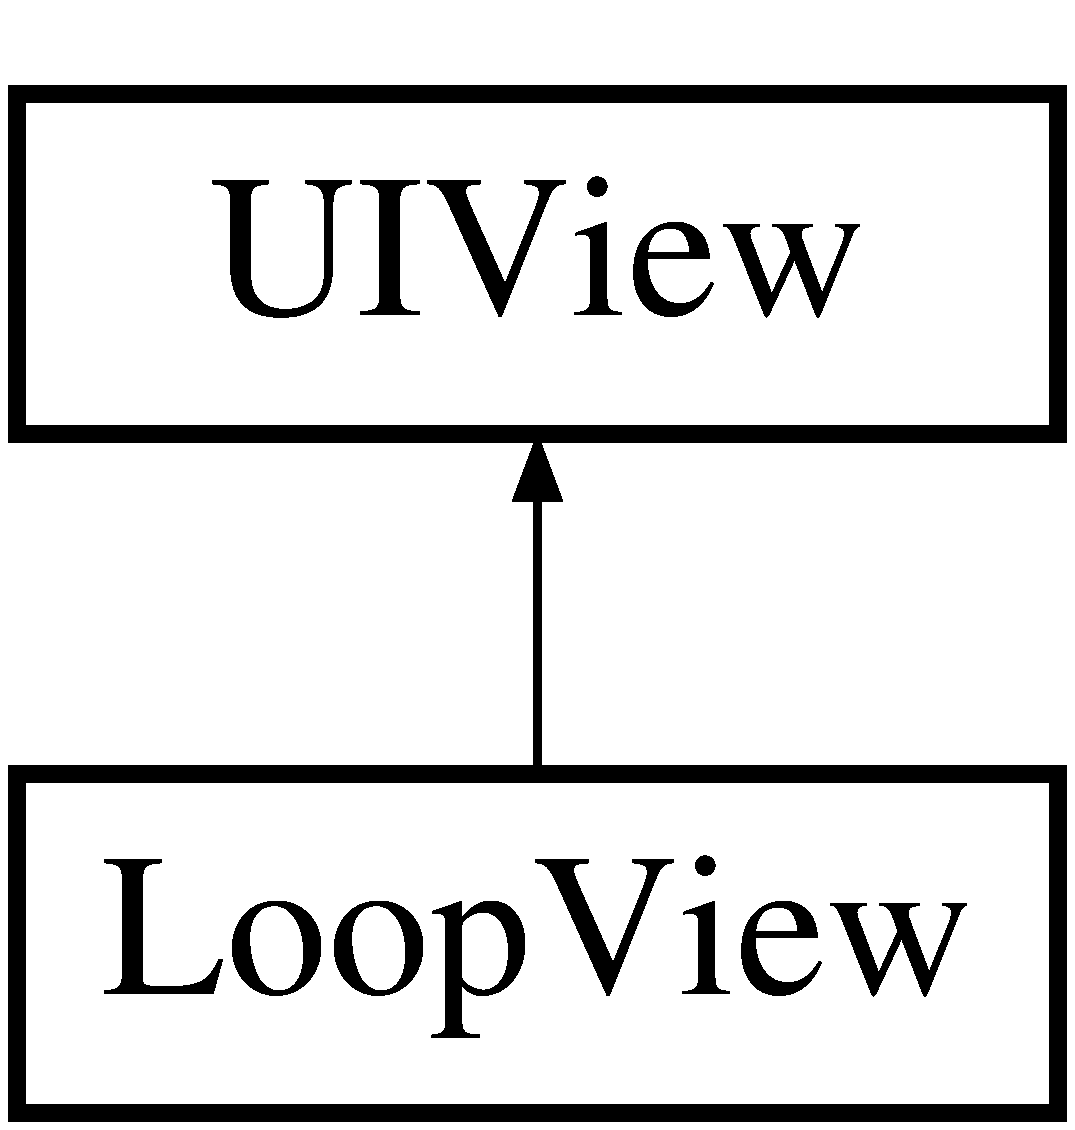
\includegraphics[height=2.000000cm]{interface_loop_view}
\end{center}
\end{figure}
\subsection*{Instance Methods}
\begin{DoxyCompactItemize}
\item 
(id) -\/ \hyperlink{interface_loop_view_a1e7227b1d41e651a603e80315935a3ee}{init\-With\-Frame\-:and\-Parent\-:}
\item 
(void) -\/ \hyperlink{interface_loop_view_a8c03538769a6fcbd7aa8e672cf4b5c96}{draw\-Rect\-:}
\item 
(void) -\/ \hyperlink{interface_loop_view_a2357112d7fefe9f720ac82c881236830}{touches\-Began\-:with\-Event\-:}
\item 
(void) -\/ \hyperlink{interface_loop_view_a06bf1152e9fa0dd16bf7f46128ae0cff}{touches\-Moved\-:with\-Event\-:}
\item 
(void) -\/ \hyperlink{interface_loop_view_ad9cc995e0aa0c5e28ab827a06c897c36}{touches\-Ended\-:with\-Event\-:}
\item 
(void) -\/ \hyperlink{interface_loop_view_a38393b10eebe5376725616eb446df377}{handle\-Single\-Tap\-:}
\end{DoxyCompactItemize}
\subsection*{Properties}
\begin{DoxyCompactItemize}
\item 
\hypertarget{interface_loop_view_a4b93d352d2fca75b34e1b5a50e03f587}{N\-S\-String $\ast$ \hyperlink{interface_loop_view_a4b93d352d2fca75b34e1b5a50e03f587}{name}}\label{interface_loop_view_a4b93d352d2fca75b34e1b5a50e03f587}

\begin{DoxyCompactList}\small\item\em The name of the loop. \end{DoxyCompactList}\item 
\hypertarget{interface_loop_view_a0df1d66872ef90fe830b9118e0c76202}{bool \hyperlink{interface_loop_view_a0df1d66872ef90fe830b9118e0c76202}{is\-Clockwise}}\label{interface_loop_view_a0df1d66872ef90fe830b9118e0c76202}

\begin{DoxyCompactList}\small\item\em Determines if the symbol is a clockwise loop. \end{DoxyCompactList}\item 
\hypertarget{interface_loop_view_a4376b99467d16ed71554a4a6ddd4ae0a}{id \hyperlink{interface_loop_view_a4376b99467d16ed71554a4a6ddd4ae0a}{parent}}\label{interface_loop_view_a4376b99467d16ed71554a4a6ddd4ae0a}

\begin{DoxyCompactList}\small\item\em Pointer to the parent of this view. \end{DoxyCompactList}\end{DoxyCompactItemize}


\subsection{Detailed Description}
A view that contains the graphical representation of a \hyperlink{interface_loop}{Loop}. 

\subsection{Method Documentation}
\hypertarget{interface_loop_view_a8c03538769a6fcbd7aa8e672cf4b5c96}{\index{Loop\-View@{Loop\-View}!draw\-Rect\-:@{draw\-Rect\-:}}
\index{draw\-Rect\-:@{draw\-Rect\-:}!LoopView@{Loop\-View}}
\subsubsection[{draw\-Rect\-:}]{\setlength{\rightskip}{0pt plus 5cm}-\/ (void) draw\-Rect\-: 
\begin{DoxyParamCaption}
\item[{(C\-G\-Rect)}]{rect}
\end{DoxyParamCaption}
}}\label{interface_loop_view_a8c03538769a6fcbd7aa8e672cf4b5c96}
Draws the receiver’s image within the passed-\/in rectangle. This is an overridden method. 
\begin{DoxyParams}{Parameters}
{\em rect} & the frame of the view in which objects can be drawn. \\
\hline
\end{DoxyParams}
\hypertarget{interface_loop_view_a38393b10eebe5376725616eb446df377}{\index{Loop\-View@{Loop\-View}!handle\-Single\-Tap\-:@{handle\-Single\-Tap\-:}}
\index{handle\-Single\-Tap\-:@{handle\-Single\-Tap\-:}!LoopView@{Loop\-View}}
\subsubsection[{handle\-Single\-Tap\-:}]{\setlength{\rightskip}{0pt plus 5cm}-\/ (void) handle\-Single\-Tap\-: 
\begin{DoxyParamCaption}
\item[{(U\-I\-Tap\-Gesture\-Recognizer $\ast$)}]{sender}
\end{DoxyParamCaption}
}}\label{interface_loop_view_a38393b10eebe5376725616eb446df377}
Will open up the menu of options for the object on a single tap. 
\begin{DoxyParams}{Parameters}
{\em sender} & the recognizer that fired the method call. \\
\hline
\end{DoxyParams}
\hypertarget{interface_loop_view_a1e7227b1d41e651a603e80315935a3ee}{\index{Loop\-View@{Loop\-View}!init\-With\-Frame\-:and\-Parent\-:@{init\-With\-Frame\-:and\-Parent\-:}}
\index{init\-With\-Frame\-:and\-Parent\-:@{init\-With\-Frame\-:and\-Parent\-:}!LoopView@{Loop\-View}}
\subsubsection[{init\-With\-Frame\-:and\-Parent\-:}]{\setlength{\rightskip}{0pt plus 5cm}-\/ (id) init\-With\-Frame\-: 
\begin{DoxyParamCaption}
\item[{(C\-G\-Rect)}]{frame}
\item[{andParent:(id)}]{parent}
\end{DoxyParamCaption}
}}\label{interface_loop_view_a1e7227b1d41e651a603e80315935a3ee}
Initializes the view. 
\begin{DoxyParams}{Parameters}
{\em frame} & the frame the view is contained within. \\
\hline
{\em parent} & a pointer to the parent object that holds the view. \\
\hline
\end{DoxyParams}
\begin{DoxyReturn}{Returns}
an id of the newly created view 
\end{DoxyReturn}
\hypertarget{interface_loop_view_a2357112d7fefe9f720ac82c881236830}{\index{Loop\-View@{Loop\-View}!touches\-Began\-:with\-Event\-:@{touches\-Began\-:with\-Event\-:}}
\index{touches\-Began\-:with\-Event\-:@{touches\-Began\-:with\-Event\-:}!LoopView@{Loop\-View}}
\subsubsection[{touches\-Began\-:with\-Event\-:}]{\setlength{\rightskip}{0pt plus 5cm}-\/ (void) touches\-Began\-: 
\begin{DoxyParamCaption}
\item[{(N\-S\-Set $\ast$)}]{touches}
\item[{withEvent:(U\-I\-Event $\ast$)}]{event}
\end{DoxyParamCaption}
}}\label{interface_loop_view_a2357112d7fefe9f720ac82c881236830}
Logs event at the beginning of moving the loop. 
\begin{DoxyParams}{Parameters}
{\em touches} & the set of touch events registered by the application. \\
\hline
{\em event} & the U\-I\-Event that fired the the method call. \\
\hline
\end{DoxyParams}
\hypertarget{interface_loop_view_ad9cc995e0aa0c5e28ab827a06c897c36}{\index{Loop\-View@{Loop\-View}!touches\-Ended\-:with\-Event\-:@{touches\-Ended\-:with\-Event\-:}}
\index{touches\-Ended\-:with\-Event\-:@{touches\-Ended\-:with\-Event\-:}!LoopView@{Loop\-View}}
\subsubsection[{touches\-Ended\-:with\-Event\-:}]{\setlength{\rightskip}{0pt plus 5cm}-\/ (void) touches\-Ended\-: 
\begin{DoxyParamCaption}
\item[{(N\-S\-Set $\ast$)}]{touches}
\item[{withEvent:(U\-I\-Event $\ast$)}]{event}
\end{DoxyParamCaption}
}}\label{interface_loop_view_ad9cc995e0aa0c5e28ab827a06c897c36}
Logs event at the end of moving the loop. 
\begin{DoxyParams}{Parameters}
{\em touches} & the set of touch events registered by the application. \\
\hline
{\em event} & the U\-I\-Event that fired the the method call. \\
\hline
\end{DoxyParams}
\hypertarget{interface_loop_view_a06bf1152e9fa0dd16bf7f46128ae0cff}{\index{Loop\-View@{Loop\-View}!touches\-Moved\-:with\-Event\-:@{touches\-Moved\-:with\-Event\-:}}
\index{touches\-Moved\-:with\-Event\-:@{touches\-Moved\-:with\-Event\-:}!LoopView@{Loop\-View}}
\subsubsection[{touches\-Moved\-:with\-Event\-:}]{\setlength{\rightskip}{0pt plus 5cm}-\/ (void) touches\-Moved\-: 
\begin{DoxyParamCaption}
\item[{(N\-S\-Set $\ast$)}]{touches}
\item[{withEvent:(U\-I\-Event $\ast$)}]{event}
\end{DoxyParamCaption}
}}\label{interface_loop_view_a06bf1152e9fa0dd16bf7f46128ae0cff}
Handles moving the loop object across the view when the user drags the object. 
\begin{DoxyParams}{Parameters}
{\em touches} & the set of touch events registered by the application. \\
\hline
{\em event} & the U\-I\-Event that fired the the method call. \\
\hline
\end{DoxyParams}


The documentation for this class was generated from the following files\-:\begin{DoxyCompactItemize}
\item 
Group\-Modeling\-App/Loop\-View.\-h\item 
Group\-Modeling\-App/Loop\-View.\-m\end{DoxyCompactItemize}

\hypertarget{interface_m_f_side_menu_container_view_controller}{\section{M\-F\-Side\-Menu\-Container\-View\-Controller Class Reference}
\label{interface_m_f_side_menu_container_view_controller}\index{M\-F\-Side\-Menu\-Container\-View\-Controller@{M\-F\-Side\-Menu\-Container\-View\-Controller}}
}
Inheritance diagram for M\-F\-Side\-Menu\-Container\-View\-Controller\-:\begin{figure}[H]
\begin{center}
\leavevmode
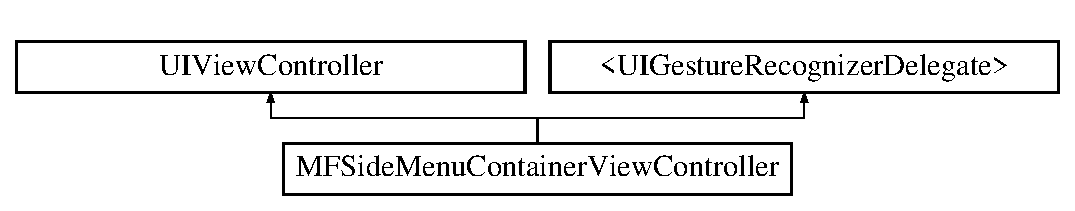
\includegraphics[height=2.000000cm]{interface_m_f_side_menu_container_view_controller}
\end{center}
\end{figure}
\subsection*{Instance Methods}
\begin{DoxyCompactItemize}
\item 
\hypertarget{interface_m_f_side_menu_container_view_controller_a14def1b095d58eadd905ed12be837526}{(void) -\/ \hyperlink{interface_m_f_side_menu_container_view_controller_a14def1b095d58eadd905ed12be837526}{open\-Help\-Section}}\label{interface_m_f_side_menu_container_view_controller_a14def1b095d58eadd905ed12be837526}

\begin{DoxyCompactList}\small\item\em Pushes the help section view controller onto the stack making it visible. \end{DoxyCompactList}\item 
\hypertarget{interface_m_f_side_menu_container_view_controller_a3a8b7ec3ac60d621cbf41613b8be4977}{(void) -\/ \hyperlink{interface_m_f_side_menu_container_view_controller_a3a8b7ec3ac60d621cbf41613b8be4977}{return\-To\-Root}}\label{interface_m_f_side_menu_container_view_controller_a3a8b7ec3ac60d621cbf41613b8be4977}

\begin{DoxyCompactList}\small\item\em Pops back to the root view controller which will be the model. \end{DoxyCompactList}\item 
\hypertarget{interface_m_f_side_menu_container_view_controller_ab0deb7fe845f3f889cab59cdce30413b}{(void) -\/ {\bfseries toggle\-Left\-Side\-Menu\-Completion\-:}}\label{interface_m_f_side_menu_container_view_controller_ab0deb7fe845f3f889cab59cdce30413b}

\item 
\hypertarget{interface_m_f_side_menu_container_view_controller_a7e73bdb0e4c6ac09cd15a282a31e866f}{(void) -\/ {\bfseries set\-Menu\-State\-:completion\-:}}\label{interface_m_f_side_menu_container_view_controller_a7e73bdb0e4c6ac09cd15a282a31e866f}

\item 
\hypertarget{interface_m_f_side_menu_container_view_controller_a69177c8c40668aa71e60a23ae975de3b}{(void) -\/ {\bfseries set\-Menu\-Width\-:animated\-:}}\label{interface_m_f_side_menu_container_view_controller_a69177c8c40668aa71e60a23ae975de3b}

\item 
\hypertarget{interface_m_f_side_menu_container_view_controller_a57209e9a2c33ce3433427a7903da4367}{(void) -\/ {\bfseries set\-Left\-Menu\-Width\-:animated\-:}}\label{interface_m_f_side_menu_container_view_controller_a57209e9a2c33ce3433427a7903da4367}

\end{DoxyCompactItemize}
\subsection*{Class Methods}
\begin{DoxyCompactItemize}
\item 
(\hyperlink{interface_m_f_side_menu_container_view_controller}{M\-F\-Side\-Menu\-Container\-View\-Controller} $\ast$) + \hyperlink{interface_m_f_side_menu_container_view_controller_a8dd4ba3c4452eb18fe9bfe73aebd978a}{container\-With\-Center\-View\-Controller\-:left\-Menu\-View\-Controller\-:}
\end{DoxyCompactItemize}
\subsection*{Properties}
\begin{DoxyCompactItemize}
\item 
\hypertarget{interface_m_f_side_menu_container_view_controller_a49e8e7e16a8d53b0e0c4378994c3abe5}{U\-I\-Navigation\-Controller $\ast$ {\bfseries center\-View\-Controller}}\label{interface_m_f_side_menu_container_view_controller_a49e8e7e16a8d53b0e0c4378994c3abe5}

\item 
\hypertarget{interface_m_f_side_menu_container_view_controller_a048098d93fef8397e4419e77d697b521}{U\-I\-View\-Controller $\ast$ {\bfseries left\-Menu\-View\-Controller}}\label{interface_m_f_side_menu_container_view_controller_a048098d93fef8397e4419e77d697b521}

\item 
\hypertarget{interface_m_f_side_menu_container_view_controller_a4ee6f366285ae4e3b63af91d8aeed278}{M\-F\-Side\-Menu\-State {\bfseries menu\-State}}\label{interface_m_f_side_menu_container_view_controller_a4ee6f366285ae4e3b63af91d8aeed278}

\item 
\hypertarget{interface_m_f_side_menu_container_view_controller_aee44d69de8e8ce0550b7302d69c5558a}{M\-F\-Side\-Menu\-Pan\-Mode {\bfseries pan\-Mode}}\label{interface_m_f_side_menu_container_view_controller_aee44d69de8e8ce0550b7302d69c5558a}

\item 
\hypertarget{interface_m_f_side_menu_container_view_controller_a342f7eaf6e1081866b0020cc21004798}{C\-G\-Float {\bfseries menu\-Animation\-Default\-Duration}}\label{interface_m_f_side_menu_container_view_controller_a342f7eaf6e1081866b0020cc21004798}

\item 
\hypertarget{interface_m_f_side_menu_container_view_controller_aa7cfc1198278935cb2ec2f24896ffac1}{C\-G\-Float {\bfseries menu\-Animation\-Max\-Duration}}\label{interface_m_f_side_menu_container_view_controller_aa7cfc1198278935cb2ec2f24896ffac1}

\item 
\hypertarget{interface_m_f_side_menu_container_view_controller_a84e32827e2bce1c3393774bc6c084ade}{C\-G\-Float {\bfseries menu\-Width}}\label{interface_m_f_side_menu_container_view_controller_a84e32827e2bce1c3393774bc6c084ade}

\item 
\hypertarget{interface_m_f_side_menu_container_view_controller_ad4a34ce849a37f5acdcb23ed6a7e745e}{C\-G\-Float {\bfseries left\-Menu\-Width}}\label{interface_m_f_side_menu_container_view_controller_ad4a34ce849a37f5acdcb23ed6a7e745e}

\item 
\hypertarget{interface_m_f_side_menu_container_view_controller_abb51782bddbe51511e4e9ed0bf48048d}{B\-O\-O\-L {\bfseries shadow\-Enabled}}\label{interface_m_f_side_menu_container_view_controller_abb51782bddbe51511e4e9ed0bf48048d}

\item 
\hypertarget{interface_m_f_side_menu_container_view_controller_af0f3c352b73af28b000459cb754541b1}{C\-G\-Float {\bfseries shadow\-Radius}}\label{interface_m_f_side_menu_container_view_controller_af0f3c352b73af28b000459cb754541b1}

\item 
\hypertarget{interface_m_f_side_menu_container_view_controller_a850ca4f7b12e4210f803c24ece6b7e0c}{C\-G\-Float {\bfseries shadow\-Opacity}}\label{interface_m_f_side_menu_container_view_controller_a850ca4f7b12e4210f803c24ece6b7e0c}

\item 
\hypertarget{interface_m_f_side_menu_container_view_controller_aebef02c51c68b688a74b905cfbe7ecac}{U\-I\-Color $\ast$ {\bfseries shadow\-Color}}\label{interface_m_f_side_menu_container_view_controller_aebef02c51c68b688a74b905cfbe7ecac}

\item 
\hypertarget{interface_m_f_side_menu_container_view_controller_a291bcae1d839e9308389ae3f3721b883}{B\-O\-O\-L {\bfseries menu\-Slide\-Animation\-Enabled}}\label{interface_m_f_side_menu_container_view_controller_a291bcae1d839e9308389ae3f3721b883}

\item 
\hypertarget{interface_m_f_side_menu_container_view_controller_ae6d8aee0f4015d7b9022ad51518dae63}{C\-G\-Float {\bfseries menu\-Slide\-Animation\-Factor}}\label{interface_m_f_side_menu_container_view_controller_ae6d8aee0f4015d7b9022ad51518dae63}

\end{DoxyCompactItemize}


\subsection{Method Documentation}
\hypertarget{interface_m_f_side_menu_container_view_controller_a8dd4ba3c4452eb18fe9bfe73aebd978a}{\index{M\-F\-Side\-Menu\-Container\-View\-Controller@{M\-F\-Side\-Menu\-Container\-View\-Controller}!container\-With\-Center\-View\-Controller\-:left\-Menu\-View\-Controller\-:@{container\-With\-Center\-View\-Controller\-:left\-Menu\-View\-Controller\-:}}
\index{container\-With\-Center\-View\-Controller\-:left\-Menu\-View\-Controller\-:@{container\-With\-Center\-View\-Controller\-:left\-Menu\-View\-Controller\-:}!MFSideMenuContainerViewController@{M\-F\-Side\-Menu\-Container\-View\-Controller}}
\subsubsection[{container\-With\-Center\-View\-Controller\-:left\-Menu\-View\-Controller\-:}]{\setlength{\rightskip}{0pt plus 5cm}+ ({\bf M\-F\-Side\-Menu\-Container\-View\-Controller} $\ast$) container\-With\-Center\-View\-Controller\-: 
\begin{DoxyParamCaption}
\item[{(id)}]{center\-View\-Controller}
\item[{leftMenuViewController:(id)}]{left\-Menu\-View\-Controller}
\end{DoxyParamCaption}
}}\label{interface_m_f_side_menu_container_view_controller_a8dd4ba3c4452eb18fe9bfe73aebd978a}
Creates a container with a left side menu and a center working view controller. 
\begin{DoxyParams}{Parameters}
{\em center\-View\-Controller} & the view controller for the center. \\
\hline
{\em left\-Menu\-View\-Controller} & the view controller for the side menu. \\
\hline
\end{DoxyParams}
\begin{DoxyReturn}{Returns}
an instance of \hyperlink{interface_m_f_side_menu_container_view_controller}{M\-F\-Side\-Menu\-Container\-View\-Controller}. 
\end{DoxyReturn}


The documentation for this class was generated from the following files\-:\begin{DoxyCompactItemize}
\item 
Group\-Modeling\-App/M\-F\-Side\-Menu\-Container\-View\-Controller.\-h\item 
Group\-Modeling\-App/M\-F\-Side\-Menu\-Container\-View\-Controller.\-m\end{DoxyCompactItemize}

\hypertarget{category_m_f_side_menu_container_view_controller_07_08}{\section{M\-F\-Side\-Menu\-Container\-View\-Controller() Category Reference}
\label{category_m_f_side_menu_container_view_controller_07_08}\index{M\-F\-Side\-Menu\-Container\-View\-Controller()@{M\-F\-Side\-Menu\-Container\-View\-Controller()}}
}
\subsection*{Properties}
\begin{DoxyCompactItemize}
\item 
\hypertarget{category_m_f_side_menu_container_view_controller_07_08_ace43610b9ba71ee914c426728caebcb7}{U\-I\-View $\ast$ {\bfseries menu\-Container\-View}}\label{category_m_f_side_menu_container_view_controller_07_08_ace43610b9ba71ee914c426728caebcb7}

\item 
\hypertarget{category_m_f_side_menu_container_view_controller_07_08_ab22b3ae21049ea6126b3399910c458f3}{C\-G\-Point {\bfseries pan\-Gesture\-Origin}}\label{category_m_f_side_menu_container_view_controller_07_08_ab22b3ae21049ea6126b3399910c458f3}

\item 
\hypertarget{category_m_f_side_menu_container_view_controller_07_08_a2fee6262ec666a3ba9ef6712a5f56b86}{C\-G\-Float {\bfseries pan\-Gesture\-Velocity}}\label{category_m_f_side_menu_container_view_controller_07_08_a2fee6262ec666a3ba9ef6712a5f56b86}

\item 
\hypertarget{category_m_f_side_menu_container_view_controller_07_08_ac99172d884a172137c0bd03e5eee0e68}{M\-F\-Side\-Menu\-Pan\-Direction {\bfseries pan\-Direction}}\label{category_m_f_side_menu_container_view_controller_07_08_ac99172d884a172137c0bd03e5eee0e68}

\end{DoxyCompactItemize}


The documentation for this category was generated from the following file\-:\begin{DoxyCompactItemize}
\item 
Group\-Modeling\-App/M\-F\-Side\-Menu\-Container\-View\-Controller.\-m\end{DoxyCompactItemize}

\hypertarget{interface_model}{\section{Model Class Reference}
\label{interface_model}\index{Model@{Model}}
}


This class is responsible for holding all aspects of a causal loop diagram model. This includes all causal links, variables, feedback loops, simulation parameters, and default parameters.  




{\ttfamily \#import $<$Model.\-h$>$}

Inheritance diagram for Model\-:\begin{figure}[H]
\begin{center}
\leavevmode
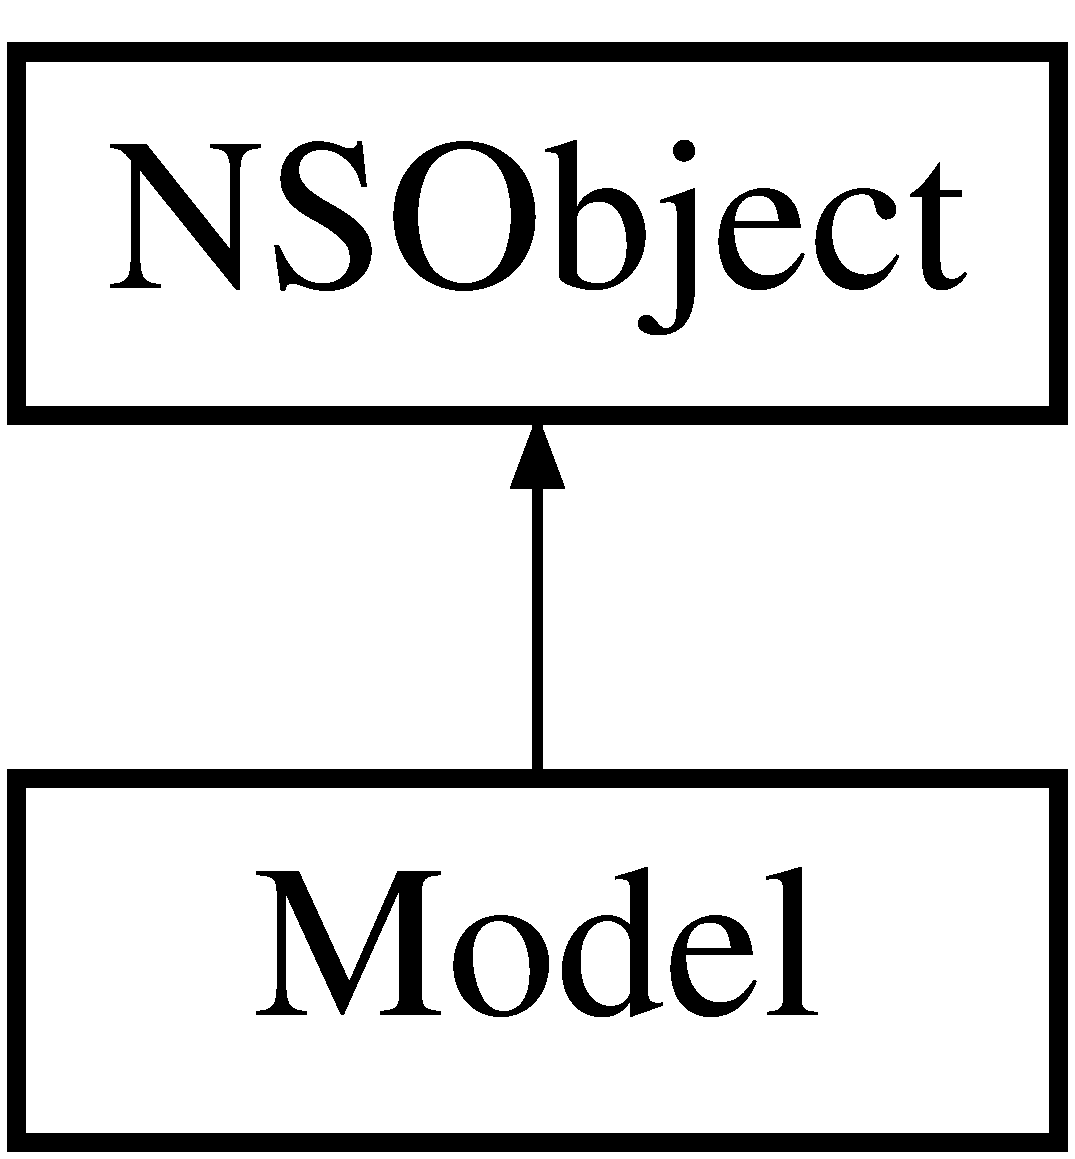
\includegraphics[height=2.000000cm]{interface_model}
\end{center}
\end{figure}
\subsection*{Instance Methods}
\begin{DoxyCompactItemize}
\item 
(void) -\/ \hyperlink{interface_model_a1aa9ffd361768e65dff67ca34bece31e}{clear\-Model}
\begin{DoxyCompactList}\small\item\em Clears the model when you need to create or load a brand new file. \end{DoxyCompactList}\item 
(N\-S\-String $\ast$) -\/ \hyperlink{interface_model_a91805a3382a6a5e971b6ba41cf239d13}{construct\-Location\-Details\-:}
\item 
(N\-S\-Mutable\-Array $\ast$) -\/ \hyperlink{interface_model_a11e5b56412cf5554242194f97c3f0289}{create\-Variable\-Map}
\item 
(N\-S\-Mutable\-Array $\ast$) -\/ \hyperlink{interface_model_a4a8949c3a08298f59357fd8e23da5b4e}{create\-Components\-Export}
\item 
(int) -\/ \hyperlink{interface_model_adc802e370fc8db1828ab0720ccf1b421}{add\-Casual\-Link\-With\-Parent\-:and\-Child\-:}
\item 
(void) -\/ \hyperlink{interface_model_a47282c90df52a90537c270e38f7ab896}{add\-Component\-:}
\item 
(int) -\/ \hyperlink{interface_model_af6d6ffe8413a0199fa4810a378023496}{delete\-Causal\-Link\-:}
\item 
(int) -\/ \hyperlink{interface_model_aa4479c88b7241e0f24079c0318d37b54}{delete\-Loop\-:}
\item 
(int) -\/ \hyperlink{interface_model_a6a9cee44b5ea8954538199c1ceb07eff}{delete\-Variable\-:}
\item 
(U\-I\-View $\ast$) -\/ \hyperlink{interface_model_ab40d7b555b5fd0c7306b1035fa959158}{get\-View\-Controller\-View}
\item 
(U\-I\-View\-Controller $\ast$) -\/ \hyperlink{interface_model_aa36ee992fc98c9ef079d6b8954299479}{get\-View\-Controller}
\item 
(\hyperlink{interface_variable}{Variable} $\ast$) -\/ \hyperlink{interface_model_a9ccc4c0d1f6d72f49cdd2e105607d71a}{get\-Variable\-:}
\item 
(\hyperlink{interface_variable}{Variable} $\ast$) -\/ \hyperlink{interface_model_ab7e33b4b1a19e36620ba81922065ec22}{get\-Variable\-At\-Point\-:}
\item 
(void) -\/ \hyperlink{interface_model_aface1baeb2283622b46ce5725fbd3064}{move\-Variable\-:}
\item 
(void) -\/ \hyperlink{interface_model_a9417e1d438a60f39d050eb0dfc500a72}{set\-Variable\-Color\-:}
\item 
(C\-G\-Rect) -\/ \hyperlink{interface_model_a462b730c3f085149c45b1901fbb924ca}{find\-Model\-Frame}
\end{DoxyCompactItemize}
\subsection*{Class Methods}
\begin{DoxyCompactItemize}
\item 
(\hyperlink{interface_model}{Model} $\ast$) + \hyperlink{interface_model_a4f1d39e1881443e4ecd87d660e9c91b4}{shared\-Model}
\end{DoxyCompactItemize}
\subsection*{Properties}
\begin{DoxyCompactItemize}
\item 
\hypertarget{interface_model_a84e232bb9b9692876f48dc2e95c8c2ab}{N\-S\-Mutable\-Array $\ast$ \hyperlink{interface_model_a84e232bb9b9692876f48dc2e95c8c2ab}{components}}\label{interface_model_a84e232bb9b9692876f48dc2e95c8c2ab}

\begin{DoxyCompactList}\small\item\em An array that contains all variables, causal links, and feedback loops of the model. \end{DoxyCompactList}\item 
\hypertarget{interface_model_a4be35dd9732f61e8d31f36497e615ac4}{\hyperlink{interface_default_parameters}{Default\-Parameters} $\ast$ \hyperlink{interface_model_a4be35dd9732f61e8d31f36497e615ac4}{default\-Params}}\label{interface_model_a4be35dd9732f61e8d31f36497e615ac4}

\begin{DoxyCompactList}\small\item\em An instance of \hyperlink{interface_default_parameters}{Default\-Parameters} which contains the Vensim default parameters for the model such as font and size. \end{DoxyCompactList}\item 
\hypertarget{interface_model_a2be19c9425d7cfdc74424a9afbdbd9de}{\hyperlink{interface_control_parameters}{Control\-Parameters} $\ast$ \hyperlink{interface_model_a2be19c9425d7cfdc74424a9afbdbd9de}{control\-Params}}\label{interface_model_a2be19c9425d7cfdc74424a9afbdbd9de}

\begin{DoxyCompactList}\small\item\em An instance of \hyperlink{interface_control_parameters}{Control\-Parameters} which contains the Vensim control parameters which specify how the simulation runs. \end{DoxyCompactList}\item 
\hypertarget{interface_model_ad6dba38c5d11da948afdddbd0a6e2caa}{N\-S\-Data $\ast$ \hyperlink{interface_model_ad6dba38c5d11da948afdddbd0a6e2caa}{starting\-Hash}}\label{interface_model_ad6dba38c5d11da948afdddbd0a6e2caa}

\begin{DoxyCompactList}\small\item\em A hash string of the file that was imported from Dropbox. Will be null if brand new file. \end{DoxyCompactList}\item 
\hypertarget{interface_model_a3a3aa4972b9e878cf839228535944a82}{N\-S\-Data $\ast$ \hyperlink{interface_model_a3a3aa4972b9e878cf839228535944a82}{ending\-Hash}}\label{interface_model_a3a3aa4972b9e878cf839228535944a82}

\begin{DoxyCompactList}\small\item\em A hash string of the file that was exported to Dropbox. \end{DoxyCompactList}\end{DoxyCompactItemize}


\subsection{Detailed Description}
This class is responsible for holding all aspects of a causal loop diagram model. This includes all causal links, variables, feedback loops, simulation parameters, and default parameters. 

\subsection{Method Documentation}
\hypertarget{interface_model_adc802e370fc8db1828ab0720ccf1b421}{\index{Model@{Model}!add\-Casual\-Link\-With\-Parent\-:and\-Child\-:@{add\-Casual\-Link\-With\-Parent\-:and\-Child\-:}}
\index{add\-Casual\-Link\-With\-Parent\-:and\-Child\-:@{add\-Casual\-Link\-With\-Parent\-:and\-Child\-:}!Model@{Model}}
\subsubsection[{add\-Casual\-Link\-With\-Parent\-:and\-Child\-:}]{\setlength{\rightskip}{0pt plus 5cm}-\/ (int) add\-Casual\-Link\-With\-Parent\-: 
\begin{DoxyParamCaption}
\item[{({\bf Variable}$\ast$)}]{parent}
\item[{andChild:({\bf Variable}$\ast$)}]{child}
\end{DoxyParamCaption}
}}\label{interface_model_adc802e370fc8db1828ab0720ccf1b421}
Will add a new causal\-Link to the model given a parent and a child. The link will be a straight line from the parent to the child. 
\begin{DoxyParams}{Parameters}
{\em parent} & the parent \hyperlink{interface_variable}{Variable} of the causal link. \\
\hline
{\em child} & the child \hyperlink{interface_variable}{Variable} of the causal link. \\
\hline
\end{DoxyParams}
\begin{DoxyReturn}{Returns}
the id number of the newly created causal link. 
\end{DoxyReturn}
\hypertarget{interface_model_a47282c90df52a90537c270e38f7ab896}{\index{Model@{Model}!add\-Component\-:@{add\-Component\-:}}
\index{add\-Component\-:@{add\-Component\-:}!Model@{Model}}
\subsubsection[{add\-Component\-:}]{\setlength{\rightskip}{0pt plus 5cm}-\/ (void) add\-Component\-: 
\begin{DoxyParamCaption}
\item[{(id)}]{obj}
\end{DoxyParamCaption}
}}\label{interface_model_a47282c90df52a90537c270e38f7ab896}
Adds a newly created object to the list of components existing in the model. 
\begin{DoxyParams}{Parameters}
{\em obj} & an object that needs to be added to the model. Will be either a \hyperlink{interface_causal_link}{Causal\-Link}, \hyperlink{interface_variable}{Variable} or a \hyperlink{interface_loop}{Loop}. \\
\hline
\end{DoxyParams}
\hypertarget{interface_model_a1aa9ffd361768e65dff67ca34bece31e}{\index{Model@{Model}!clear\-Model@{clear\-Model}}
\index{clear\-Model@{clear\-Model}!Model@{Model}}
\subsubsection[{clear\-Model}]{\setlength{\rightskip}{0pt plus 5cm}-\/ (void) clear\-Model 
\begin{DoxyParamCaption}
{}
\end{DoxyParamCaption}
}}\label{interface_model_a1aa9ffd361768e65dff67ca34bece31e}


Clears the model when you need to create or load a brand new file. 

\begin{DoxyNote}{Note}
do not think i want to do this here... Will erase initial condtions when a user tries to open a file. Need to detemine when event lists are cleared. 
\end{DoxyNote}
\hypertarget{interface_model_a91805a3382a6a5e971b6ba41cf239d13}{\index{Model@{Model}!construct\-Location\-Details\-:@{construct\-Location\-Details\-:}}
\index{construct\-Location\-Details\-:@{construct\-Location\-Details\-:}!Model@{Model}}
\subsubsection[{construct\-Location\-Details\-:}]{\setlength{\rightskip}{0pt plus 5cm}-\/ (N\-S\-String $\ast$) construct\-Location\-Details\-: 
\begin{DoxyParamCaption}
\item[{(C\-G\-Point)}]{location}
\end{DoxyParamCaption}
}}\label{interface_model_a91805a3382a6a5e971b6ba41cf239d13}
Constructs the details message for all moving events. 
\begin{DoxyParams}{Parameters}
{\em location} & the point where the object is located. \\
\hline
\end{DoxyParams}
\begin{DoxyReturn}{Returns}
a string with the location. 
\end{DoxyReturn}
\hypertarget{interface_model_a4a8949c3a08298f59357fd8e23da5b4e}{\index{Model@{Model}!create\-Components\-Export@{create\-Components\-Export}}
\index{create\-Components\-Export@{create\-Components\-Export}!Model@{Model}}
\subsubsection[{create\-Components\-Export}]{\setlength{\rightskip}{0pt plus 5cm}-\/ (N\-S\-Mutable\-Array $\ast$) create\-Components\-Export 
\begin{DoxyParamCaption}
{}
\end{DoxyParamCaption}
}}\label{interface_model_a4a8949c3a08298f59357fd8e23da5b4e}
Constructs a list of output strings for every component. \begin{DoxyReturn}{Returns}
an array of output strings for all components. 
\end{DoxyReturn}
\hypertarget{interface_model_a11e5b56412cf5554242194f97c3f0289}{\index{Model@{Model}!create\-Variable\-Map@{create\-Variable\-Map}}
\index{create\-Variable\-Map@{create\-Variable\-Map}!Model@{Model}}
\subsubsection[{create\-Variable\-Map}]{\setlength{\rightskip}{0pt plus 5cm}-\/ (N\-S\-Mutable\-Array $\ast$) create\-Variable\-Map 
\begin{DoxyParamCaption}
{}
\end{DoxyParamCaption}
}}\label{interface_model_a11e5b56412cf5554242194f97c3f0289}
Iterates over all of the Variables in the model and constructs the Vensim Function of() map for each one. \begin{DoxyReturn}{Returns}
an array of strings that hold all of the output text of the variable maps. 
\end{DoxyReturn}
\hypertarget{interface_model_af6d6ffe8413a0199fa4810a378023496}{\index{Model@{Model}!delete\-Causal\-Link\-:@{delete\-Causal\-Link\-:}}
\index{delete\-Causal\-Link\-:@{delete\-Causal\-Link\-:}!Model@{Model}}
\subsubsection[{delete\-Causal\-Link\-:}]{\setlength{\rightskip}{0pt plus 5cm}-\/ (int) delete\-Causal\-Link\-: 
\begin{DoxyParamCaption}
\item[{(id)}]{link\-View}
\end{DoxyParamCaption}
}}\label{interface_model_af6d6ffe8413a0199fa4810a378023496}
Searches the list of components for a \hyperlink{interface_causal_link}{Causal\-Link} component with a specified \hyperlink{interface_causal_link_view}{Causal\-Link\-View}. 
\begin{DoxyParams}{Parameters}
{\em link\-View} & the view associated with the Casual\-Link. \\
\hline
\end{DoxyParams}
\begin{DoxyReturn}{Returns}
the id numbder of the causal link that was deleted for logging purposes. 
\end{DoxyReturn}
\hypertarget{interface_model_aa4479c88b7241e0f24079c0318d37b54}{\index{Model@{Model}!delete\-Loop\-:@{delete\-Loop\-:}}
\index{delete\-Loop\-:@{delete\-Loop\-:}!Model@{Model}}
\subsubsection[{delete\-Loop\-:}]{\setlength{\rightskip}{0pt plus 5cm}-\/ (int) delete\-Loop\-: 
\begin{DoxyParamCaption}
\item[{(id)}]{loop\-View}
\end{DoxyParamCaption}
}}\label{interface_model_aa4479c88b7241e0f24079c0318d37b54}
Searched the list of components for a \hyperlink{interface_loop}{Loop} component with a specified \hyperlink{interface_loop_view}{Loop\-View}. 
\begin{DoxyParams}{Parameters}
{\em loop\-View} & the view associated with the \hyperlink{interface_loop}{Loop}. \\
\hline
\end{DoxyParams}
\begin{DoxyReturn}{Returns}
the id numbder of the loop that was deleted for logging purposes. 
\end{DoxyReturn}
\hypertarget{interface_model_a6a9cee44b5ea8954538199c1ceb07eff}{\index{Model@{Model}!delete\-Variable\-:@{delete\-Variable\-:}}
\index{delete\-Variable\-:@{delete\-Variable\-:}!Model@{Model}}
\subsubsection[{delete\-Variable\-:}]{\setlength{\rightskip}{0pt plus 5cm}-\/ (int) delete\-Variable\-: 
\begin{DoxyParamCaption}
\item[{(id)}]{variable\-View}
\end{DoxyParamCaption}
}}\label{interface_model_a6a9cee44b5ea8954538199c1ceb07eff}
Searched the list of components for a \hyperlink{interface_variable}{Variable} component with a specified \hyperlink{interface_variable_view}{Variable\-View}. 
\begin{DoxyParams}{Parameters}
{\em variable\-View} & the view associated with the \hyperlink{interface_variable}{Variable}. \\
\hline
\end{DoxyParams}
\begin{DoxyReturn}{Returns}
the id numbder of the variable that was deleted for logging purposes. 
\end{DoxyReturn}
\hypertarget{interface_model_a462b730c3f085149c45b1901fbb924ca}{\index{Model@{Model}!find\-Model\-Frame@{find\-Model\-Frame}}
\index{find\-Model\-Frame@{find\-Model\-Frame}!Model@{Model}}
\subsubsection[{find\-Model\-Frame}]{\setlength{\rightskip}{0pt plus 5cm}-\/ (C\-G\-Rect) find\-Model\-Frame 
\begin{DoxyParamCaption}
{}
\end{DoxyParamCaption}
}}\label{interface_model_a462b730c3f085149c45b1901fbb924ca}
Will find the smallest frame that will contain the entire model. Used for taking pictures of the model. \begin{DoxyReturn}{Returns}
a C\-G\-Rect of the frame of the entire model. 
\end{DoxyReturn}
\hypertarget{interface_model_a9ccc4c0d1f6d72f49cdd2e105607d71a}{\index{Model@{Model}!get\-Variable\-:@{get\-Variable\-:}}
\index{get\-Variable\-:@{get\-Variable\-:}!Model@{Model}}
\subsubsection[{get\-Variable\-:}]{\setlength{\rightskip}{0pt plus 5cm}-\/ ({\bf Variable} $\ast$) get\-Variable\-: 
\begin{DoxyParamCaption}
\item[{(N\-S\-Number$\ast$)}]{id\-Number}
\end{DoxyParamCaption}
}}\label{interface_model_a9ccc4c0d1f6d72f49cdd2e105607d71a}
Searches the list of components for a \hyperlink{interface_variable}{Variable} component with a specified id. 
\begin{DoxyParams}{Parameters}
{\em id\-Number} & the id number of the \hyperlink{interface_variable}{Variable} that is being searched for. \\
\hline
\end{DoxyParams}
\begin{DoxyReturn}{Returns}
a pointer to a variable object with an id of id\-Number. 
\end{DoxyReturn}
\hypertarget{interface_model_ab7e33b4b1a19e36620ba81922065ec22}{\index{Model@{Model}!get\-Variable\-At\-Point\-:@{get\-Variable\-At\-Point\-:}}
\index{get\-Variable\-At\-Point\-:@{get\-Variable\-At\-Point\-:}!Model@{Model}}
\subsubsection[{get\-Variable\-At\-Point\-:}]{\setlength{\rightskip}{0pt plus 5cm}-\/ ({\bf Variable} $\ast$) get\-Variable\-At\-Point\-: 
\begin{DoxyParamCaption}
\item[{(C\-G\-Point)}]{point}
\end{DoxyParamCaption}
}}\label{interface_model_ab7e33b4b1a19e36620ba81922065ec22}
Searches the list of components for a \hyperlink{interface_variable}{Variable} component that contains the provided point. 
\begin{DoxyParams}{Parameters}
{\em point} & the point within the superview frame. \\
\hline
\end{DoxyParams}
\begin{DoxyReturn}{Returns}
pointer to a \hyperlink{interface_variable}{Variable} object that contains the point, nil if none do. 
\end{DoxyReturn}
\hypertarget{interface_model_aa36ee992fc98c9ef079d6b8954299479}{\index{Model@{Model}!get\-View\-Controller@{get\-View\-Controller}}
\index{get\-View\-Controller@{get\-View\-Controller}!Model@{Model}}
\subsubsection[{get\-View\-Controller}]{\setlength{\rightskip}{0pt plus 5cm}-\/ (U\-I\-View\-Controller $\ast$) get\-View\-Controller 
\begin{DoxyParamCaption}
{}
\end{DoxyParamCaption}
}}\label{interface_model_aa36ee992fc98c9ef079d6b8954299479}
Gets the view controller. \begin{DoxyReturn}{Returns}
a pointer to the currently displayed view controller. 
\end{DoxyReturn}
\hypertarget{interface_model_ab40d7b555b5fd0c7306b1035fa959158}{\index{Model@{Model}!get\-View\-Controller\-View@{get\-View\-Controller\-View}}
\index{get\-View\-Controller\-View@{get\-View\-Controller\-View}!Model@{Model}}
\subsubsection[{get\-View\-Controller\-View}]{\setlength{\rightskip}{0pt plus 5cm}-\/ (U\-I\-View $\ast$) get\-View\-Controller\-View 
\begin{DoxyParamCaption}
{}
\end{DoxyParamCaption}
}}\label{interface_model_ab40d7b555b5fd0c7306b1035fa959158}
Gets the root view controller view. \begin{DoxyReturn}{Returns}
the currently displayed view controller view from the app delegate. 
\end{DoxyReturn}
\hypertarget{interface_model_aface1baeb2283622b46ce5725fbd3064}{\index{Model@{Model}!move\-Variable\-:@{move\-Variable\-:}}
\index{move\-Variable\-:@{move\-Variable\-:}!Model@{Model}}
\subsubsection[{move\-Variable\-:}]{\setlength{\rightskip}{0pt plus 5cm}-\/ (void) move\-Variable\-: 
\begin{DoxyParamCaption}
\item[{(id)}]{variable\-View}
\end{DoxyParamCaption}
}}\label{interface_model_aface1baeb2283622b46ce5725fbd3064}
Searches the list of components for a \hyperlink{interface_variable}{Variable} component with a specified \hyperlink{interface_variable_view}{Variable\-View} and will move the attached Causal\-Links. 
\begin{DoxyParams}{Parameters}
{\em variable\-View} & the view associated with the \hyperlink{interface_variable}{Variable}. \\
\hline
\end{DoxyParams}
\hypertarget{interface_model_a9417e1d438a60f39d050eb0dfc500a72}{\index{Model@{Model}!set\-Variable\-Color\-:@{set\-Variable\-Color\-:}}
\index{set\-Variable\-Color\-:@{set\-Variable\-Color\-:}!Model@{Model}}
\subsubsection[{set\-Variable\-Color\-:}]{\setlength{\rightskip}{0pt plus 5cm}-\/ (void) set\-Variable\-Color\-: 
\begin{DoxyParamCaption}
\item[{(C\-G\-Point)}]{location}
\end{DoxyParamCaption}
}}\label{interface_model_a9417e1d438a60f39d050eb0dfc500a72}
Will iterate over all of the variables in the model and make a call to determine if the provided point lies within the bounds of the variable's view frame to change the box color. This is used when a user is creating a new causal link. 
\begin{DoxyParams}{Parameters}
{\em location} & the point in the coordinate space user to determine if a variable contains that point. \\
\hline
\end{DoxyParams}
\hypertarget{interface_model_a4f1d39e1881443e4ecd87d660e9c91b4}{\index{Model@{Model}!shared\-Model@{shared\-Model}}
\index{shared\-Model@{shared\-Model}!Model@{Model}}
\subsubsection[{shared\-Model}]{\setlength{\rightskip}{0pt plus 5cm}+ ({\bf Model} $\ast$) shared\-Model 
\begin{DoxyParamCaption}
{}
\end{DoxyParamCaption}
}}\label{interface_model_a4f1d39e1881443e4ecd87d660e9c91b4}
Forces the \hyperlink{interface_model}{Model} to be a singleton class. \begin{DoxyReturn}{Returns}
a pointer to the single instance of the model. 
\end{DoxyReturn}


The documentation for this class was generated from the following files\-:\begin{DoxyCompactItemize}
\item 
Group\-Modeling\-App/Model.\-h\item 
Group\-Modeling\-App/Model.\-m\end{DoxyCompactItemize}

\hypertarget{interface_model_section_view}{\section{Model\-Section\-View Class Reference}
\label{interface_model_section_view}\index{Model\-Section\-View@{Model\-Section\-View}}
}


A view that displays the \hyperlink{interface_model}{Model} and allows for modifications to the model.  




{\ttfamily \#import $<$Model\-Section\-View.\-h$>$}

Inheritance diagram for Model\-Section\-View\-:\begin{figure}[H]
\begin{center}
\leavevmode
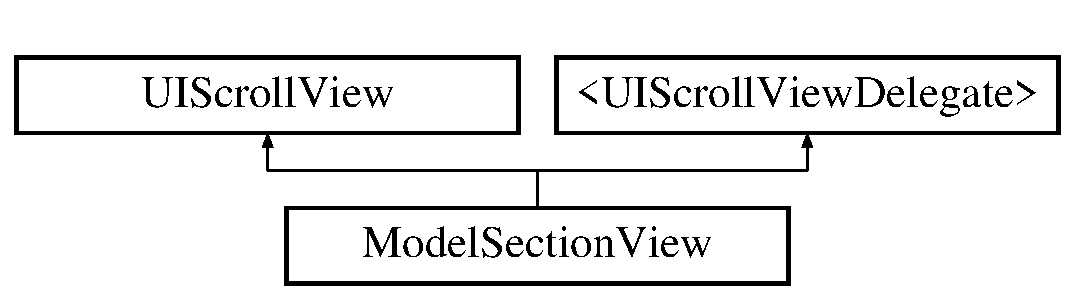
\includegraphics[height=2.000000cm]{interface_model_section_view}
\end{center}
\end{figure}
\subsection*{Instance Methods}
\begin{DoxyCompactItemize}
\item 
(id) -\/ \hyperlink{interface_model_section_view_a4213bb26f5207ee3f402fe463badc691}{init}
\item 
(void) -\/ \hyperlink{interface_model_section_view_a8c03538769a6fcbd7aa8e672cf4b5c96}{draw\-Rect\-:}
\item 
(void) -\/ \hyperlink{interface_model_section_view_abe37687ff567bae7bca561f22b7a1802}{handle\-Double\-Tap\-:}
\item 
(U\-I\-View $\ast$) -\/ \hyperlink{interface_model_section_view_ac1af4c1c7381cee5560d9ddebdf8203a}{hit\-Test\-:with\-Event\-:}
\item 
(void) -\/ \hyperlink{interface_model_section_view_aad6be714d494a1b1bfd3e148ac1ff13b}{scroll\-View\-Will\-Begin\-Dragging\-:}
\item 
(void) -\/ \hyperlink{interface_model_section_view_a863eaf47ffa7b051ba103a60fc8bfdf8}{scroll\-View\-Did\-Scroll\-:}
\item 
(void) -\/ \hyperlink{interface_model_section_view_ab8c0489df0e1103bd844273e1f31cd9e}{scroll\-View\-Did\-End\-Dragging\-:will\-Decelerate\-:}
\item 
(void) -\/ \hyperlink{interface_model_section_view_a33f55893a32225b60aba8e51445250c6}{scroll\-View\-Did\-End\-Decelerating\-:}
\end{DoxyCompactItemize}


\subsection{Detailed Description}
A view that displays the \hyperlink{interface_model}{Model} and allows for modifications to the model. 

\subsection{Method Documentation}
\hypertarget{interface_model_section_view_a8c03538769a6fcbd7aa8e672cf4b5c96}{\index{Model\-Section\-View@{Model\-Section\-View}!draw\-Rect\-:@{draw\-Rect\-:}}
\index{draw\-Rect\-:@{draw\-Rect\-:}!ModelSectionView@{Model\-Section\-View}}
\subsubsection[{draw\-Rect\-:}]{\setlength{\rightskip}{0pt plus 5cm}-\/ (void) draw\-Rect\-: 
\begin{DoxyParamCaption}
\item[{(C\-G\-Rect)}]{rect}
\end{DoxyParamCaption}
}}\label{interface_model_section_view_a8c03538769a6fcbd7aa8e672cf4b5c96}
Draws the receiver’s image within the passed-\/in rectangle. This is an overridden method. 
\begin{DoxyParams}{Parameters}
{\em rect} & the frame of the view in which objects can be drawn. \\
\hline
\end{DoxyParams}
\hypertarget{interface_model_section_view_abe37687ff567bae7bca561f22b7a1802}{\index{Model\-Section\-View@{Model\-Section\-View}!handle\-Double\-Tap\-:@{handle\-Double\-Tap\-:}}
\index{handle\-Double\-Tap\-:@{handle\-Double\-Tap\-:}!ModelSectionView@{Model\-Section\-View}}
\subsubsection[{handle\-Double\-Tap\-:}]{\setlength{\rightskip}{0pt plus 5cm}-\/ (void) handle\-Double\-Tap\-: 
\begin{DoxyParamCaption}
\item[{(U\-I\-Tap\-Gesture\-Recognizer $\ast$)}]{sender}
\end{DoxyParamCaption}
}}\label{interface_model_section_view_abe37687ff567bae7bca561f22b7a1802}
Will add a new object on a double tap. 
\begin{DoxyParams}{Parameters}
{\em sender} & the recognizer that fired the method call. \\
\hline
\end{DoxyParams}
\hypertarget{interface_model_section_view_ac1af4c1c7381cee5560d9ddebdf8203a}{\index{Model\-Section\-View@{Model\-Section\-View}!hit\-Test\-:with\-Event\-:@{hit\-Test\-:with\-Event\-:}}
\index{hit\-Test\-:with\-Event\-:@{hit\-Test\-:with\-Event\-:}!ModelSectionView@{Model\-Section\-View}}
\subsubsection[{hit\-Test\-:with\-Event\-:}]{\setlength{\rightskip}{0pt plus 5cm}-\/ (U\-I\-View $\ast$) hit\-Test\-: 
\begin{DoxyParamCaption}
\item[{(C\-G\-Point)}]{point}
\item[{withEvent:(U\-I\-Event $\ast$)}]{event}
\end{DoxyParamCaption}
}}\label{interface_model_section_view_ac1af4c1c7381cee5560d9ddebdf8203a}
Used to determine if the event is for the scroll view or any associated subview 
\begin{DoxyParams}{Parameters}
{\em point} & the point at which the user has touched. \\
\hline
{\em event} & the event that triggered this method call. \\
\hline
\end{DoxyParams}
\begin{DoxyReturn}{Returns}
the view object that is the farthest descendent the current view and contains point. Returns nil if the point lies completely outside the receiver’s view hierarchy. 
\end{DoxyReturn}
\hypertarget{interface_model_section_view_a4213bb26f5207ee3f402fe463badc691}{\index{Model\-Section\-View@{Model\-Section\-View}!init@{init}}
\index{init@{init}!ModelSectionView@{Model\-Section\-View}}
\subsubsection[{init}]{\setlength{\rightskip}{0pt plus 5cm}-\/ (id) init 
\begin{DoxyParamCaption}
{}
\end{DoxyParamCaption}
}}\label{interface_model_section_view_a4213bb26f5207ee3f402fe463badc691}
Initializes the view. 
\begin{DoxyParams}{Parameters}
{\em frame} & the frame the view is contained within. \\
\hline
\end{DoxyParams}
\begin{DoxyReturn}{Returns}
an id of the newly created view. 
\end{DoxyReturn}
\hypertarget{interface_model_section_view_a33f55893a32225b60aba8e51445250c6}{\index{Model\-Section\-View@{Model\-Section\-View}!scroll\-View\-Did\-End\-Decelerating\-:@{scroll\-View\-Did\-End\-Decelerating\-:}}
\index{scroll\-View\-Did\-End\-Decelerating\-:@{scroll\-View\-Did\-End\-Decelerating\-:}!ModelSectionView@{Model\-Section\-View}}
\subsubsection[{scroll\-View\-Did\-End\-Decelerating\-:}]{\setlength{\rightskip}{0pt plus 5cm}-\/ (void) scroll\-View\-Did\-End\-Decelerating\-: 
\begin{DoxyParamCaption}
\item[{(U\-I\-Scroll\-View $\ast$)}]{scroll\-View}
\end{DoxyParamCaption}
}}\label{interface_model_section_view_a33f55893a32225b60aba8e51445250c6}
Notifies the logger that the scroll window has stopped scrolling. The user may have simply released their finger or swiped their finger. 
\begin{DoxyParams}{Parameters}
{\em scroll\-View} & the scrollview for which the event has occured. \\
\hline
\end{DoxyParams}
\hypertarget{interface_model_section_view_ab8c0489df0e1103bd844273e1f31cd9e}{\index{Model\-Section\-View@{Model\-Section\-View}!scroll\-View\-Did\-End\-Dragging\-:will\-Decelerate\-:@{scroll\-View\-Did\-End\-Dragging\-:will\-Decelerate\-:}}
\index{scroll\-View\-Did\-End\-Dragging\-:will\-Decelerate\-:@{scroll\-View\-Did\-End\-Dragging\-:will\-Decelerate\-:}!ModelSectionView@{Model\-Section\-View}}
\subsubsection[{scroll\-View\-Did\-End\-Dragging\-:will\-Decelerate\-:}]{\setlength{\rightskip}{0pt plus 5cm}-\/ (void) scroll\-View\-Did\-End\-Dragging\-: 
\begin{DoxyParamCaption}
\item[{(U\-I\-Scroll\-View $\ast$)}]{scroll\-View}
\item[{willDecelerate:(B\-O\-O\-L)}]{decelerate}
\end{DoxyParamCaption}
}}\label{interface_model_section_view_ab8c0489df0e1103bd844273e1f31cd9e}
Notifies the logger that the user has stopped dragging the scrollview. 
\begin{DoxyParams}{Parameters}
{\em scroll\-View} & the scrollview for which the event has occured. \\
\hline
{\em decelerate} & T\-R\-U\-E if the scrolling will continue because the user has swiped their finger. F\-A\-L\-S\-E if the user simply released their finger. \\
\hline
\end{DoxyParams}
\hypertarget{interface_model_section_view_a863eaf47ffa7b051ba103a60fc8bfdf8}{\index{Model\-Section\-View@{Model\-Section\-View}!scroll\-View\-Did\-Scroll\-:@{scroll\-View\-Did\-Scroll\-:}}
\index{scroll\-View\-Did\-Scroll\-:@{scroll\-View\-Did\-Scroll\-:}!ModelSectionView@{Model\-Section\-View}}
\subsubsection[{scroll\-View\-Did\-Scroll\-:}]{\setlength{\rightskip}{0pt plus 5cm}-\/ (void) scroll\-View\-Did\-Scroll\-: 
\begin{DoxyParamCaption}
\item[{(U\-I\-Scroll\-View $\ast$)}]{scroll\-View}
\end{DoxyParamCaption}
}}\label{interface_model_section_view_a863eaf47ffa7b051ba103a60fc8bfdf8}
Notifies the logger that the user is scrolling. 
\begin{DoxyParams}{Parameters}
{\em scroll\-View} & the scrollview for which the event has occured. \\
\hline
\end{DoxyParams}
\hypertarget{interface_model_section_view_aad6be714d494a1b1bfd3e148ac1ff13b}{\index{Model\-Section\-View@{Model\-Section\-View}!scroll\-View\-Will\-Begin\-Dragging\-:@{scroll\-View\-Will\-Begin\-Dragging\-:}}
\index{scroll\-View\-Will\-Begin\-Dragging\-:@{scroll\-View\-Will\-Begin\-Dragging\-:}!ModelSectionView@{Model\-Section\-View}}
\subsubsection[{scroll\-View\-Will\-Begin\-Dragging\-:}]{\setlength{\rightskip}{0pt plus 5cm}-\/ (void) scroll\-View\-Will\-Begin\-Dragging\-: 
\begin{DoxyParamCaption}
\item[{(U\-I\-Scroll\-View $\ast$)}]{scroll\-View}
\end{DoxyParamCaption}
}}\label{interface_model_section_view_aad6be714d494a1b1bfd3e148ac1ff13b}
Notifies the logger that the user has begun scrolling. 
\begin{DoxyParams}{Parameters}
{\em scroll\-View} & the scrollview for which the event has occured. \\
\hline
\end{DoxyParams}


The documentation for this class was generated from the following files\-:\begin{DoxyCompactItemize}
\item 
Group\-Modeling\-App/Model\-Section\-View.\-h\item 
Group\-Modeling\-App/Model\-Section\-View.\-m\end{DoxyCompactItemize}

\hypertarget{interface_model_section_view_controller}{\section{Model\-Section\-View\-Controller Class Reference}
\label{interface_model_section_view_controller}\index{Model\-Section\-View\-Controller@{Model\-Section\-View\-Controller}}
}


The view controller that handles interaction with the model section.  




{\ttfamily \#import $<$Model\-Section\-View\-Controller.\-h$>$}

Inheritance diagram for Model\-Section\-View\-Controller\-:\begin{figure}[H]
\begin{center}
\leavevmode
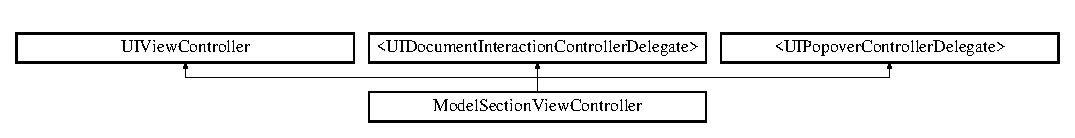
\includegraphics[height=1.403509cm]{interface_model_section_view_controller}
\end{center}
\end{figure}
\subsection*{Instance Methods}
\begin{DoxyCompactItemize}
\item 
(id) -\/ \hyperlink{interface_model_section_view_controller_a4213bb26f5207ee3f402fe463badc691}{init}
\item 
(void) -\/ \hyperlink{interface_model_section_view_controller_aa58593cee765899b690466d15042bf77}{reachability\-Changed\-:}
\item 
(void) -\/ \hyperlink{interface_model_section_view_controller_ab5dd369587af6b3abdd89f312624875f}{check\-Internet\-Connection\-:}
\item 
(void) -\/ \hyperlink{interface_model_section_view_controller_a8331227f39fd462d9e4eb04f06c2a91b}{load\-Model}
\item 
\hypertarget{interface_model_section_view_controller_a6383afe43bdf71c9197a5723793b1fb8}{(void) -\/ \hyperlink{interface_model_section_view_controller_a6383afe43bdf71c9197a5723793b1fb8}{new\-Model}}\label{interface_model_section_view_controller_a6383afe43bdf71c9197a5723793b1fb8}

\begin{DoxyCompactList}\small\item\em Will create a blank sheet so that the user can create a new model. \end{DoxyCompactList}\item 
(void) -\/ \hyperlink{interface_model_section_view_controller_a0052cb4e8c2d69372b8750f3cba55b7f}{take\-Picture\-Of\-Model}
\item 
(void) -\/ \hyperlink{interface_model_section_view_controller_a0910163cad75578d1000ea69340980bf}{image\-:did\-Finish\-Saving\-With\-Error\-:context\-Info\-:}
\item 
(void) -\/ \hyperlink{interface_model_section_view_controller_aa5a50adbd2b567d3a8ae3445329b70d1}{view\-Did\-Load}
\item 
(void) -\/ \hyperlink{interface_model_section_view_controller_a8991afe6ce31445caafbbc84338898c1}{reenable\-Save\-Button}
\item 
\hypertarget{interface_model_section_view_controller_a887a799bad6860d3fd09e0d52cb78d12}{(void) -\/ \hyperlink{interface_model_section_view_controller_a887a799bad6860d3fd09e0d52cb78d12}{save\-Model}}\label{interface_model_section_view_controller_a887a799bad6860d3fd09e0d52cb78d12}

\begin{DoxyCompactList}\small\item\em Will save the current model. \end{DoxyCompactList}\item 
(\hyperlink{interface_m_f_side_menu_container_view_controller}{M\-F\-Side\-Menu\-Container\-View\-Controller} $\ast$) -\/ \hyperlink{interface_model_section_view_controller_ad9f497773e1c2f5e420929a60f3bf7df}{menu\-Container\-View\-Controller}
\item 
(void) -\/ \hyperlink{interface_model_section_view_controller_a9644bcb73520daa217ad0709b0e6bd64}{setup\-Menu\-Bar\-Button\-Items}
\begin{DoxyCompactList}\small\item\em Sets up the menu bar of the view controller. \end{DoxyCompactList}\item 
(U\-I\-Bar\-Button\-Item $\ast$) -\/ \hyperlink{interface_model_section_view_controller_afb11718c8a0c6f7abd85dfbc7adb1cd1}{left\-Menu\-Bar\-Button\-Item}
\item 
(N\-S\-Array $\ast$) -\/ \hyperlink{interface_model_section_view_controller_a78c969d7bca3de65268ac706059e291c}{right\-Menu\-Bar\-Button\-Items}
\item 
(void) -\/ \hyperlink{interface_model_section_view_controller_a738b842dc5261f08da93880f0b006b55}{left\-Side\-Menu\-Button\-Pressed\-:}
\item 
(B\-O\-O\-L) -\/ \hyperlink{interface_model_section_view_controller_ade65ba8ae784e35b1f2b23a55afbbf9b}{can\-Become\-First\-Responder}
\item 
(B\-O\-O\-L) -\/ \hyperlink{interface_model_section_view_controller_a4a5338d3a62ac53d52a2b31880b6802c}{can\-Perform\-Action\-:with\-Sender\-:}
\item 
(void) -\/ \hyperlink{interface_model_section_view_controller_a8a501e57528492cf6ba20c9c966282e0}{create\-Update\-Menu\-:}
\item 
\hypertarget{interface_model_section_view_controller_aa7642eed869c29236ca6198804aa9624}{(void) -\/ \hyperlink{interface_model_section_view_controller_aa7642eed869c29236ca6198804aa9624}{did\-Hide\-Update\-Menu}}\label{interface_model_section_view_controller_aa7642eed869c29236ca6198804aa9624}

\begin{DoxyCompactList}\small\item\em Will log a message stating the update menu closed. \end{DoxyCompactList}\item 
(void) -\/ \hyperlink{interface_model_section_view_controller_a831a0780f91825e4c91b2116d8806c33}{create\-Edit\-Menu\-:}
\item 
(C\-G\-Rect) -\/ \hyperlink{interface_model_section_view_controller_a3ce01e8eb3a6a32185225e1bfa51454d}{get\-Variable\-Vertex\-View\-:}
\item 
(U\-I\-Toolbar $\ast$) -\/ \hyperlink{interface_model_section_view_controller_a6a24750238ea3d59bb706b8d46e1f4c4}{create\-Edit\-Menu\-Toolbar\-:}
\item 
(void) -\/ \hyperlink{interface_model_section_view_controller_ade8553713185dc0c75c1d6f543eaa54f}{popover\-Controller\-Did\-Dismiss\-Popover\-:}
\item 
\hypertarget{interface_model_section_view_controller_acb15a33593297fd02f940207a504f2a7}{(void) -\/ \hyperlink{interface_model_section_view_controller_acb15a33593297fd02f940207a504f2a7}{save\-Changes}}\label{interface_model_section_view_controller_acb15a33593297fd02f940207a504f2a7}

\begin{DoxyCompactList}\small\item\em Will save the changes made by the user related to the object they changed. \end{DoxyCompactList}\item 
(void) -\/ \hyperlink{interface_model_section_view_controller_a2ba2c7e577a0ca5fc873237ba423f514}{alert\-View\-:clicked\-Button\-At\-Index\-:}
\item 
(void) -\/ \hyperlink{interface_model_section_view_controller_ab68e5fd03354e4a1dd1a2a75ff93dbea}{show\-Delete\-Alert\-:}
\item 
(int) -\/ \hyperlink{interface_model_section_view_controller_a1dcc9249f1500714ff1b5a63b8de3982}{get\-Selected\-View\-I\-D\-Num}
\item 
(void) -\/ \hyperlink{interface_model_section_view_controller_afc53a5989b05a1405e9ac226bb05d52c}{document\-Interaction\-Controller\-Will\-Present\-Open\-In\-Menu\-:}
\item 
(void) -\/ \hyperlink{interface_model_section_view_controller_abc178903c0b14db15612cb4a3108aacc}{document\-Interaction\-Controller\-Did\-Dismiss\-Open\-In\-Menu\-:}
\item 
(void) -\/ \hyperlink{interface_model_section_view_controller_abdb08679098f7e6ac87ead9b47dd67fa}{document\-Interaction\-Controller\-:will\-Begin\-Sending\-To\-Application\-:}
\item 
\hypertarget{interface_model_section_view_controller_ae780db37d3f6bcefbebeced10969ed12}{(void) -\/ \hyperlink{interface_model_section_view_controller_ae780db37d3f6bcefbebeced10969ed12}{menu\-Change}}\label{interface_model_section_view_controller_ae780db37d3f6bcefbebeced10969ed12}

\begin{DoxyCompactList}\small\item\em Notifies the logger when a new option from the segmented control has been changed. \end{DoxyCompactList}\item 
(N\-S\-String $\ast$) -\/ \hyperlink{interface_model_section_view_controller_a165de32a7bdbc801f76d3a61012d0679}{get\-Menu\-Details}
\end{DoxyCompactItemize}
\subsection*{Properties}
\begin{DoxyCompactItemize}
\item 
\hypertarget{interface_model_section_view_controller_a1160a302c7d1456b2232508e66bf74f3}{U\-I\-Segmented\-Control $\ast$ \hyperlink{interface_model_section_view_controller_a1160a302c7d1456b2232508e66bf74f3}{controls}}\label{interface_model_section_view_controller_a1160a302c7d1456b2232508e66bf74f3}

\begin{DoxyCompactList}\small\item\em The menu of options to add new objects to the model. \end{DoxyCompactList}\item 
\hypertarget{interface_model_section_view_controller_a6177c3f5ef7ae97e8a88fb845c4d5fd5}{U\-I\-Bar\-Button\-Item $\ast$ \hyperlink{interface_model_section_view_controller_a6177c3f5ef7ae97e8a88fb845c4d5fd5}{create\-New\-Button}}\label{interface_model_section_view_controller_a6177c3f5ef7ae97e8a88fb845c4d5fd5}

\begin{DoxyCompactList}\small\item\em The button that will allow a user to create a new project. \end{DoxyCompactList}\item 
\hypertarget{interface_model_section_view_controller_a770f2666d890b557d2e94ba5e1c2cbbf}{U\-I\-Segmented\-Control $\ast$ \hyperlink{interface_model_section_view_controller_a770f2666d890b557d2e94ba5e1c2cbbf}{load\-Seg\-Control}}\label{interface_model_section_view_controller_a770f2666d890b557d2e94ba5e1c2cbbf}

\begin{DoxyCompactList}\small\item\em Segmented control for loading a model. Need it so we can disable actions and change the image. \end{DoxyCompactList}\item 
\hypertarget{interface_model_section_view_controller_a4f48727f24dc50cb5241226fe2e5300b}{U\-I\-Bar\-Button\-Item $\ast$ \hyperlink{interface_model_section_view_controller_a4f48727f24dc50cb5241226fe2e5300b}{load\-Button}}\label{interface_model_section_view_controller_a4f48727f24dc50cb5241226fe2e5300b}

\begin{DoxyCompactList}\small\item\em The button that will load saved files. \end{DoxyCompactList}\item 
\hypertarget{interface_model_section_view_controller_a21477dfcf454e9177d5fb3bd04b389e9}{U\-I\-Bar\-Button\-Item $\ast$ \hyperlink{interface_model_section_view_controller_a21477dfcf454e9177d5fb3bd04b389e9}{take\-Picture\-Button}}\label{interface_model_section_view_controller_a21477dfcf454e9177d5fb3bd04b389e9}

\begin{DoxyCompactList}\small\item\em The button that will save files. \end{DoxyCompactList}\item 
\hypertarget{interface_model_section_view_controller_a1e94870fc426dba899cad9070651e562}{U\-I\-Segmented\-Control $\ast$ \hyperlink{interface_model_section_view_controller_a1e94870fc426dba899cad9070651e562}{save\-Seg\-Control}}\label{interface_model_section_view_controller_a1e94870fc426dba899cad9070651e562}

\begin{DoxyCompactList}\small\item\em Segmented control for saving a model. Need it so we can disable actions and change the image. \end{DoxyCompactList}\item 
\hypertarget{interface_model_section_view_controller_a30e5aecd252bb0cf8095e3d435b07b29}{U\-I\-Bar\-Button\-Item $\ast$ \hyperlink{interface_model_section_view_controller_a30e5aecd252bb0cf8095e3d435b07b29}{save\-Button}}\label{interface_model_section_view_controller_a30e5aecd252bb0cf8095e3d435b07b29}

\begin{DoxyCompactList}\small\item\em The button that will save files. \end{DoxyCompactList}\item 
\hypertarget{interface_model_section_view_controller_a4f6ad6ee733bbd0760d2825f6a5ce9f4}{U\-I\-Popover\-Controller $\ast$ \hyperlink{interface_model_section_view_controller_a4f6ad6ee733bbd0760d2825f6a5ce9f4}{pop\-Over\-Controller}}\label{interface_model_section_view_controller_a4f6ad6ee733bbd0760d2825f6a5ce9f4}

\begin{DoxyCompactList}\small\item\em A pointer to a U\-I\-Popover\-Controller which will contain the edit object menu. \end{DoxyCompactList}\item 
\hypertarget{interface_model_section_view_controller_a7d349fc947db08dd56690582423a4b1b}{U\-I\-View $\ast$ \hyperlink{interface_model_section_view_controller_a7d349fc947db08dd56690582423a4b1b}{selected\-View}}\label{interface_model_section_view_controller_a7d349fc947db08dd56690582423a4b1b}

\begin{DoxyCompactList}\small\item\em A pointer to the view that has been selected for menu options. \end{DoxyCompactList}\item 
\hypertarget{interface_model_section_view_controller_a9c639830cd11257200b4bdb107ce30d7}{\hyperlink{interface_model_section_view}{Model\-Section\-View} $\ast$ \hyperlink{interface_model_section_view_controller_a9c639830cd11257200b4bdb107ce30d7}{model\-View}}\label{interface_model_section_view_controller_a9c639830cd11257200b4bdb107ce30d7}

\begin{DoxyCompactList}\small\item\em A pointer to the \hyperlink{interface_model}{Model} view. \end{DoxyCompactList}\item 
\hypertarget{interface_model_section_view_controller_add10e7d857093908d7e78eda4888c848}{\hyperlink{interface_reachability}{Reachability} $\ast$ \hyperlink{interface_model_section_view_controller_add10e7d857093908d7e78eda4888c848}{internet\-Reachability}}\label{interface_model_section_view_controller_add10e7d857093908d7e78eda4888c848}

\begin{DoxyCompactList}\small\item\em A pointer to a check the internet connection of the device. \end{DoxyCompactList}\item 
\hypertarget{interface_model_section_view_controller_a40778056811a8d1ad7c407333b490120}{U\-I\-Document\-Interaction\-Controller $\ast$ \hyperlink{interface_model_section_view_controller_a40778056811a8d1ad7c407333b490120}{document\-Interaction\-Controller}}\label{interface_model_section_view_controller_a40778056811a8d1ad7c407333b490120}

\begin{DoxyCompactList}\small\item\em A pointer to the doc interaction controller to save the file. \end{DoxyCompactList}\item 
\hypertarget{interface_model_section_view_controller_a108fcdbf1198ced2d10fe789ba64f585}{dispatch\-\_\-queue\-\_\-t \hyperlink{interface_model_section_view_controller_a108fcdbf1198ced2d10fe789ba64f585}{log\-Queue}}\label{interface_model_section_view_controller_a108fcdbf1198ced2d10fe789ba64f585}

\begin{DoxyCompactList}\small\item\em An asynchronous queue that will be used to push the log files to parse. \end{DoxyCompactList}\item 
\hypertarget{interface_model_section_view_controller_a2e838e7ff8d293aa399d4c7b714b3dbc}{bool \hyperlink{interface_model_section_view_controller_a2e838e7ff8d293aa399d4c7b714b3dbc}{is\-Log\-File\-Saving}}\label{interface_model_section_view_controller_a2e838e7ff8d293aa399d4c7b714b3dbc}

\begin{DoxyCompactList}\small\item\em Will specifiy if a log file is being pushed so we do not have the save button enabled. \end{DoxyCompactList}\end{DoxyCompactItemize}


\subsection{Detailed Description}
The view controller that handles interaction with the model section. 

\subsection{Method Documentation}
\hypertarget{interface_model_section_view_controller_a2ba2c7e577a0ca5fc873237ba423f514}{\index{Model\-Section\-View\-Controller@{Model\-Section\-View\-Controller}!alert\-View\-:clicked\-Button\-At\-Index\-:@{alert\-View\-:clicked\-Button\-At\-Index\-:}}
\index{alert\-View\-:clicked\-Button\-At\-Index\-:@{alert\-View\-:clicked\-Button\-At\-Index\-:}!ModelSectionViewController@{Model\-Section\-View\-Controller}}
\subsubsection[{alert\-View\-:clicked\-Button\-At\-Index\-:}]{\setlength{\rightskip}{0pt plus 5cm}-\/ (void) alert\-View\-: 
\begin{DoxyParamCaption}
\item[{(U\-I\-Alert\-View$\ast$)}]{alert\-View}
\item[{clickedButtonAtIndex:(int)}]{index}
\end{DoxyParamCaption}
}}\label{interface_model_section_view_controller_a2ba2c7e577a0ca5fc873237ba423f514}
Handles the action of the response from the alertviews which include deleting, creating an image and creating a new model. 
\begin{DoxyParams}{Parameters}
{\em alert\-View} & the alert that has registered an action. \\
\hline
{\em index} & the index of the button selected. \\
\hline
\end{DoxyParams}
\hypertarget{interface_model_section_view_controller_ade65ba8ae784e35b1f2b23a55afbbf9b}{\index{Model\-Section\-View\-Controller@{Model\-Section\-View\-Controller}!can\-Become\-First\-Responder@{can\-Become\-First\-Responder}}
\index{can\-Become\-First\-Responder@{can\-Become\-First\-Responder}!ModelSectionViewController@{Model\-Section\-View\-Controller}}
\subsubsection[{can\-Become\-First\-Responder}]{\setlength{\rightskip}{0pt plus 5cm}-\/ (B\-O\-O\-L) can\-Become\-First\-Responder 
\begin{DoxyParamCaption}
{}
\end{DoxyParamCaption}
}}\label{interface_model_section_view_controller_ade65ba8ae784e35b1f2b23a55afbbf9b}
Determines if the reveiver can become the first responder. \begin{DoxyReturn}{Returns}
a Boolean value indicating whether the receiver can become first responder. 
\end{DoxyReturn}
\hypertarget{interface_model_section_view_controller_a4a5338d3a62ac53d52a2b31880b6802c}{\index{Model\-Section\-View\-Controller@{Model\-Section\-View\-Controller}!can\-Perform\-Action\-:with\-Sender\-:@{can\-Perform\-Action\-:with\-Sender\-:}}
\index{can\-Perform\-Action\-:with\-Sender\-:@{can\-Perform\-Action\-:with\-Sender\-:}!ModelSectionViewController@{Model\-Section\-View\-Controller}}
\subsubsection[{can\-Perform\-Action\-:with\-Sender\-:}]{\setlength{\rightskip}{0pt plus 5cm}-\/ (B\-O\-O\-L) can\-Perform\-Action\-: 
\begin{DoxyParamCaption}
\item[{(S\-E\-L)}]{action}
\item[{withSender:(id)}]{sender}
\end{DoxyParamCaption}
}}\label{interface_model_section_view_controller_a4a5338d3a62ac53d52a2b31880b6802c}
Requests the receiving responder to enable or disable the specified command in the user interface. 
\begin{DoxyParams}{Parameters}
{\em action} & a selector that identifies a method associated with a command. \\
\hline
{\em sender} & object calling this method. \\
\hline
\end{DoxyParams}
\begin{DoxyReturn}{Returns}
Y\-E\-S if the the command identified by action should be enabled or N\-O if it should be disabled. 
\end{DoxyReturn}
\hypertarget{interface_model_section_view_controller_ab5dd369587af6b3abdd89f312624875f}{\index{Model\-Section\-View\-Controller@{Model\-Section\-View\-Controller}!check\-Internet\-Connection\-:@{check\-Internet\-Connection\-:}}
\index{check\-Internet\-Connection\-:@{check\-Internet\-Connection\-:}!ModelSectionViewController@{Model\-Section\-View\-Controller}}
\subsubsection[{check\-Internet\-Connection\-:}]{\setlength{\rightskip}{0pt plus 5cm}-\/ (void) check\-Internet\-Connection\-: 
\begin{DoxyParamCaption}
\item[{({\bf Reachability} $\ast$)}]{reachability}
\end{DoxyParamCaption}
}}\label{interface_model_section_view_controller_ab5dd369587af6b3abdd89f312624875f}
Will handle \hyperlink{interface_reachability}{Reachability} notifications about internet connection. Will disable the open and save model icons when there is no internet. 
\begin{DoxyParams}{Parameters}
{\em reachability} & the Reachablity notification. \\
\hline
\end{DoxyParams}
\hypertarget{interface_model_section_view_controller_a831a0780f91825e4c91b2116d8806c33}{\index{Model\-Section\-View\-Controller@{Model\-Section\-View\-Controller}!create\-Edit\-Menu\-:@{create\-Edit\-Menu\-:}}
\index{create\-Edit\-Menu\-:@{create\-Edit\-Menu\-:}!ModelSectionViewController@{Model\-Section\-View\-Controller}}
\subsubsection[{create\-Edit\-Menu\-:}]{\setlength{\rightskip}{0pt plus 5cm}-\/ (void) create\-Edit\-Menu\-: 
\begin{DoxyParamCaption}
\item[{(U\-I\-View$\ast$)}]{sender}
\end{DoxyParamCaption}
}}\label{interface_model_section_view_controller_a831a0780f91825e4c91b2116d8806c33}
Creates the menu for editing an object. 
\begin{DoxyParams}{Parameters}
{\em sender} & the view that called to create the menu. \\
\hline
\end{DoxyParams}
\hypertarget{interface_model_section_view_controller_a6a24750238ea3d59bb706b8d46e1f4c4}{\index{Model\-Section\-View\-Controller@{Model\-Section\-View\-Controller}!create\-Edit\-Menu\-Toolbar\-:@{create\-Edit\-Menu\-Toolbar\-:}}
\index{create\-Edit\-Menu\-Toolbar\-:@{create\-Edit\-Menu\-Toolbar\-:}!ModelSectionViewController@{Model\-Section\-View\-Controller}}
\subsubsection[{create\-Edit\-Menu\-Toolbar\-:}]{\setlength{\rightskip}{0pt plus 5cm}-\/ (U\-I\-Toolbar $\ast$) create\-Edit\-Menu\-Toolbar\-: 
\begin{DoxyParamCaption}
\item[{(C\-G\-Rect)}]{frame}
\end{DoxyParamCaption}
}}\label{interface_model_section_view_controller_a6a24750238ea3d59bb706b8d46e1f4c4}
Creates the toolbar for the edit menu. 
\begin{DoxyParams}{Parameters}
{\em frame} & the frame of the toolbar. \\
\hline
\end{DoxyParams}
\begin{DoxyReturn}{Returns}
a toolbar for the edit menu containing a save and a cancel option. 
\end{DoxyReturn}
\hypertarget{interface_model_section_view_controller_a8a501e57528492cf6ba20c9c966282e0}{\index{Model\-Section\-View\-Controller@{Model\-Section\-View\-Controller}!create\-Update\-Menu\-:@{create\-Update\-Menu\-:}}
\index{create\-Update\-Menu\-:@{create\-Update\-Menu\-:}!ModelSectionViewController@{Model\-Section\-View\-Controller}}
\subsubsection[{create\-Update\-Menu\-:}]{\setlength{\rightskip}{0pt plus 5cm}-\/ (void) create\-Update\-Menu\-: 
\begin{DoxyParamCaption}
\item[{(U\-I\-View$\ast$)}]{view}
\end{DoxyParamCaption}
}}\label{interface_model_section_view_controller_a8a501e57528492cf6ba20c9c966282e0}
Creates the menu that displays the options to update the object in the model. The current update options include edit and delete. 
\begin{DoxyParams}{Parameters}
{\em view} & the view containing the object in the model. \\
\hline
\end{DoxyParams}
\hypertarget{interface_model_section_view_controller_abdb08679098f7e6ac87ead9b47dd67fa}{\index{Model\-Section\-View\-Controller@{Model\-Section\-View\-Controller}!document\-Interaction\-Controller\-:will\-Begin\-Sending\-To\-Application\-:@{document\-Interaction\-Controller\-:will\-Begin\-Sending\-To\-Application\-:}}
\index{document\-Interaction\-Controller\-:will\-Begin\-Sending\-To\-Application\-:@{document\-Interaction\-Controller\-:will\-Begin\-Sending\-To\-Application\-:}!ModelSectionViewController@{Model\-Section\-View\-Controller}}
\subsubsection[{document\-Interaction\-Controller\-:will\-Begin\-Sending\-To\-Application\-:}]{\setlength{\rightskip}{0pt plus 5cm}-\/ (void) document\-Interaction\-Controller\-: 
\begin{DoxyParamCaption}
\item[{(U\-I\-Document\-Interaction\-Controller $\ast$)}]{controller}
\item[{willBeginSendingToApplication:(N\-S\-String $\ast$)}]{application}
\end{DoxyParamCaption}
}}\label{interface_model_section_view_controller_abdb08679098f7e6ac87ead9b47dd67fa}
Logs when an option in the open menu has been selected. 
\begin{DoxyParams}{Parameters}
{\em controller} & the document interaction controller that will display the results. \\
\hline
{\em application} & a string of the application that we are being directed to. \\
\hline
\end{DoxyParams}
\hypertarget{interface_model_section_view_controller_abc178903c0b14db15612cb4a3108aacc}{\index{Model\-Section\-View\-Controller@{Model\-Section\-View\-Controller}!document\-Interaction\-Controller\-Did\-Dismiss\-Open\-In\-Menu\-:@{document\-Interaction\-Controller\-Did\-Dismiss\-Open\-In\-Menu\-:}}
\index{document\-Interaction\-Controller\-Did\-Dismiss\-Open\-In\-Menu\-:@{document\-Interaction\-Controller\-Did\-Dismiss\-Open\-In\-Menu\-:}!ModelSectionViewController@{Model\-Section\-View\-Controller}}
\subsubsection[{document\-Interaction\-Controller\-Did\-Dismiss\-Open\-In\-Menu\-:}]{\setlength{\rightskip}{0pt plus 5cm}-\/ (void) document\-Interaction\-Controller\-Did\-Dismiss\-Open\-In\-Menu\-: 
\begin{DoxyParamCaption}
\item[{(U\-I\-Document\-Interaction\-Controller $\ast$)}]{controller}
\end{DoxyParamCaption}
}}\label{interface_model_section_view_controller_abc178903c0b14db15612cb4a3108aacc}
Logs when the open in menu to save the file has been closed. 
\begin{DoxyParams}{Parameters}
{\em controller} & the document interaction controller that will display the results. \\
\hline
\end{DoxyParams}
\hypertarget{interface_model_section_view_controller_afc53a5989b05a1405e9ac226bb05d52c}{\index{Model\-Section\-View\-Controller@{Model\-Section\-View\-Controller}!document\-Interaction\-Controller\-Will\-Present\-Open\-In\-Menu\-:@{document\-Interaction\-Controller\-Will\-Present\-Open\-In\-Menu\-:}}
\index{document\-Interaction\-Controller\-Will\-Present\-Open\-In\-Menu\-:@{document\-Interaction\-Controller\-Will\-Present\-Open\-In\-Menu\-:}!ModelSectionViewController@{Model\-Section\-View\-Controller}}
\subsubsection[{document\-Interaction\-Controller\-Will\-Present\-Open\-In\-Menu\-:}]{\setlength{\rightskip}{0pt plus 5cm}-\/ (void) document\-Interaction\-Controller\-Will\-Present\-Open\-In\-Menu\-: 
\begin{DoxyParamCaption}
\item[{(U\-I\-Document\-Interaction\-Controller $\ast$)}]{controller}
\end{DoxyParamCaption}
}}\label{interface_model_section_view_controller_afc53a5989b05a1405e9ac226bb05d52c}
Logs when the open in menu to save the file is presented. 
\begin{DoxyParams}{Parameters}
{\em controller} & the document interaction controller that will display the results. \\
\hline
\end{DoxyParams}
\hypertarget{interface_model_section_view_controller_a165de32a7bdbc801f76d3a61012d0679}{\index{Model\-Section\-View\-Controller@{Model\-Section\-View\-Controller}!get\-Menu\-Details@{get\-Menu\-Details}}
\index{get\-Menu\-Details@{get\-Menu\-Details}!ModelSectionViewController@{Model\-Section\-View\-Controller}}
\subsubsection[{get\-Menu\-Details}]{\setlength{\rightskip}{0pt plus 5cm}-\/ (N\-S\-String $\ast$) get\-Menu\-Details 
\begin{DoxyParamCaption}
{}
\end{DoxyParamCaption}
}}\label{interface_model_section_view_controller_a165de32a7bdbc801f76d3a61012d0679}
Used to get the name of the class that an update/edit menu is being created for. Will be either \hyperlink{interface_variable}{Variable}, Causal Link, or \hyperlink{interface_loop}{Loop}. \begin{DoxyReturn}{Returns}
the name of the class that is being updated. 
\end{DoxyReturn}
\hypertarget{interface_model_section_view_controller_a1dcc9249f1500714ff1b5a63b8de3982}{\index{Model\-Section\-View\-Controller@{Model\-Section\-View\-Controller}!get\-Selected\-View\-I\-D\-Num@{get\-Selected\-View\-I\-D\-Num}}
\index{get\-Selected\-View\-I\-D\-Num@{get\-Selected\-View\-I\-D\-Num}!ModelSectionViewController@{Model\-Section\-View\-Controller}}
\subsubsection[{get\-Selected\-View\-I\-D\-Num}]{\setlength{\rightskip}{0pt plus 5cm}-\/ (int) get\-Selected\-View\-I\-D\-Num 
\begin{DoxyParamCaption}
{}
\end{DoxyParamCaption}
}}\label{interface_model_section_view_controller_a1dcc9249f1500714ff1b5a63b8de3982}
Given the selected view, it will return the associated id number for the object associated with that view. \begin{DoxyReturn}{Returns}
the id number of the selected view's parent. 
\end{DoxyReturn}
\hypertarget{interface_model_section_view_controller_a3ce01e8eb3a6a32185225e1bfa51454d}{\index{Model\-Section\-View\-Controller@{Model\-Section\-View\-Controller}!get\-Variable\-Vertex\-View\-:@{get\-Variable\-Vertex\-View\-:}}
\index{get\-Variable\-Vertex\-View\-:@{get\-Variable\-Vertex\-View\-:}!ModelSectionViewController@{Model\-Section\-View\-Controller}}
\subsubsection[{get\-Variable\-Vertex\-View\-:}]{\setlength{\rightskip}{0pt plus 5cm}-\/ (C\-G\-Rect) get\-Variable\-Vertex\-View\-: 
\begin{DoxyParamCaption}
\item[{({\bf Causal\-Link\-View}$\ast$)}]{view}
\end{DoxyParamCaption}
}}\label{interface_model_section_view_controller_a3ce01e8eb3a6a32185225e1bfa51454d}
Sets up the view that will place the edit menu or update menu over the vertex. 
\begin{DoxyParams}{Parameters}
{\em view} & the casual link view of the obejct we want to have a menu appear over. \\
\hline
\end{DoxyParams}
\begin{DoxyReturn}{Returns}
the rectangle frame over the vertex. 
\end{DoxyReturn}
\hypertarget{interface_model_section_view_controller_a0910163cad75578d1000ea69340980bf}{\index{Model\-Section\-View\-Controller@{Model\-Section\-View\-Controller}!image\-:did\-Finish\-Saving\-With\-Error\-:context\-Info\-:@{image\-:did\-Finish\-Saving\-With\-Error\-:context\-Info\-:}}
\index{image\-:did\-Finish\-Saving\-With\-Error\-:context\-Info\-:@{image\-:did\-Finish\-Saving\-With\-Error\-:context\-Info\-:}!ModelSectionViewController@{Model\-Section\-View\-Controller}}
\subsubsection[{image\-:did\-Finish\-Saving\-With\-Error\-:context\-Info\-:}]{\setlength{\rightskip}{0pt plus 5cm}-\/ (void) image\-: 
\begin{DoxyParamCaption}
\item[{(U\-I\-Image $\ast$)}]{image}
\item[{didFinishSavingWithError:(N\-S\-Error $\ast$)}]{error}
\item[{contextInfo:(void$\ast$)}]{context\-Info}
\end{DoxyParamCaption}
}}\label{interface_model_section_view_controller_a0910163cad75578d1000ea69340980bf}
Called after an image of the model has been saved to notify the user if the image was successfully saved. 
\begin{DoxyParams}{Parameters}
{\em image} & the image that was saved. \\
\hline
{\em did\-Finish\-Saving\-With\-Error} & whether or not there was an error when the picture was saved. \\
\hline
{\em context\-Info} & an optional pointer to any context-\/specific data that you want passed to the completion selector. \\
\hline
\end{DoxyParams}
\hypertarget{interface_model_section_view_controller_a4213bb26f5207ee3f402fe463badc691}{\index{Model\-Section\-View\-Controller@{Model\-Section\-View\-Controller}!init@{init}}
\index{init@{init}!ModelSectionViewController@{Model\-Section\-View\-Controller}}
\subsubsection[{init}]{\setlength{\rightskip}{0pt plus 5cm}-\/ (id) init 
\begin{DoxyParamCaption}
{}
\end{DoxyParamCaption}
}}\label{interface_model_section_view_controller_a4213bb26f5207ee3f402fe463badc691}
Initializes the View Controller. Will create the views for all of the menu options. \begin{DoxyReturn}{Returns}
an id of the newly created view controller. 
\end{DoxyReturn}
\hypertarget{interface_model_section_view_controller_afb11718c8a0c6f7abd85dfbc7adb1cd1}{\index{Model\-Section\-View\-Controller@{Model\-Section\-View\-Controller}!left\-Menu\-Bar\-Button\-Item@{left\-Menu\-Bar\-Button\-Item}}
\index{left\-Menu\-Bar\-Button\-Item@{left\-Menu\-Bar\-Button\-Item}!ModelSectionViewController@{Model\-Section\-View\-Controller}}
\subsubsection[{left\-Menu\-Bar\-Button\-Item}]{\setlength{\rightskip}{0pt plus 5cm}-\/ (U\-I\-Bar\-Button\-Item $\ast$) left\-Menu\-Bar\-Button\-Item 
\begin{DoxyParamCaption}
{}
\end{DoxyParamCaption}
}}\label{interface_model_section_view_controller_afb11718c8a0c6f7abd85dfbc7adb1cd1}
Creates the left menu bar button item. This item will be responsible for opening the menu. \begin{DoxyReturn}{Returns}
the left menu bar button item. 
\end{DoxyReturn}
\hypertarget{interface_model_section_view_controller_a738b842dc5261f08da93880f0b006b55}{\index{Model\-Section\-View\-Controller@{Model\-Section\-View\-Controller}!left\-Side\-Menu\-Button\-Pressed\-:@{left\-Side\-Menu\-Button\-Pressed\-:}}
\index{left\-Side\-Menu\-Button\-Pressed\-:@{left\-Side\-Menu\-Button\-Pressed\-:}!ModelSectionViewController@{Model\-Section\-View\-Controller}}
\subsubsection[{left\-Side\-Menu\-Button\-Pressed\-:}]{\setlength{\rightskip}{0pt plus 5cm}-\/ (void) left\-Side\-Menu\-Button\-Pressed\-: 
\begin{DoxyParamCaption}
\item[{(id)}]{sender}
\end{DoxyParamCaption}
}}\label{interface_model_section_view_controller_a738b842dc5261f08da93880f0b006b55}
Callback for when the left menu button is pressed. 
\begin{DoxyParams}{Parameters}
{\em sender} & the id of the sender object. \\
\hline
\end{DoxyParams}
\hypertarget{interface_model_section_view_controller_a8331227f39fd462d9e4eb04f06c2a91b}{\index{Model\-Section\-View\-Controller@{Model\-Section\-View\-Controller}!load\-Model@{load\-Model}}
\index{load\-Model@{load\-Model}!ModelSectionViewController@{Model\-Section\-View\-Controller}}
\subsubsection[{load\-Model}]{\setlength{\rightskip}{0pt plus 5cm}-\/ (void) load\-Model 
\begin{DoxyParamCaption}
{}
\end{DoxyParamCaption}
}}\label{interface_model_section_view_controller_a8331227f39fd462d9e4eb04f06c2a91b}
Called when the load model button has been pressed. This method will redirect the user to Dropbox to open a model file. \hypertarget{interface_model_section_view_controller_ad9f497773e1c2f5e420929a60f3bf7df}{\index{Model\-Section\-View\-Controller@{Model\-Section\-View\-Controller}!menu\-Container\-View\-Controller@{menu\-Container\-View\-Controller}}
\index{menu\-Container\-View\-Controller@{menu\-Container\-View\-Controller}!ModelSectionViewController@{Model\-Section\-View\-Controller}}
\subsubsection[{menu\-Container\-View\-Controller}]{\setlength{\rightskip}{0pt plus 5cm}-\/ ({\bf M\-F\-Side\-Menu\-Container\-View\-Controller} $\ast$) menu\-Container\-View\-Controller 
\begin{DoxyParamCaption}
{}
\end{DoxyParamCaption}
}}\label{interface_model_section_view_controller_ad9f497773e1c2f5e420929a60f3bf7df}
Gets the menu container view controller. \begin{DoxyReturn}{Returns}
the menu container view controller. 
\end{DoxyReturn}
\hypertarget{interface_model_section_view_controller_ade8553713185dc0c75c1d6f543eaa54f}{\index{Model\-Section\-View\-Controller@{Model\-Section\-View\-Controller}!popover\-Controller\-Did\-Dismiss\-Popover\-:@{popover\-Controller\-Did\-Dismiss\-Popover\-:}}
\index{popover\-Controller\-Did\-Dismiss\-Popover\-:@{popover\-Controller\-Did\-Dismiss\-Popover\-:}!ModelSectionViewController@{Model\-Section\-View\-Controller}}
\subsubsection[{popover\-Controller\-Did\-Dismiss\-Popover\-:}]{\setlength{\rightskip}{0pt plus 5cm}-\/ (void) popover\-Controller\-Did\-Dismiss\-Popover\-: 
\begin{DoxyParamCaption}
\item[{(U\-I\-Popover\-Controller $\ast$)}]{popover\-Controller}
\end{DoxyParamCaption}
}}\label{interface_model_section_view_controller_ade8553713185dc0c75c1d6f543eaa54f}
Dismisses the edit menu popover window if the cancel button is pressed. 
\begin{DoxyParams}{Parameters}
{\em popover\-Controller} & the popover controller that needs to be dismissed. \\
\hline
\end{DoxyParams}
\hypertarget{interface_model_section_view_controller_aa58593cee765899b690466d15042bf77}{\index{Model\-Section\-View\-Controller@{Model\-Section\-View\-Controller}!reachability\-Changed\-:@{reachability\-Changed\-:}}
\index{reachability\-Changed\-:@{reachability\-Changed\-:}!ModelSectionViewController@{Model\-Section\-View\-Controller}}
\subsubsection[{reachability\-Changed\-:}]{\setlength{\rightskip}{0pt plus 5cm}-\/ (void) reachability\-Changed\-: 
\begin{DoxyParamCaption}
\item[{(N\-S\-Notification $\ast$)}]{note}
\end{DoxyParamCaption}
}}\label{interface_model_section_view_controller_aa58593cee765899b690466d15042bf77}
Will receive notifications from \hyperlink{interface_reachability}{Reachability} and pass it off to check if the message is about internet connection. 
\begin{DoxyParams}{Parameters}
{\em note} & the notification. \\
\hline
\end{DoxyParams}
\hypertarget{interface_model_section_view_controller_a8991afe6ce31445caafbbc84338898c1}{\index{Model\-Section\-View\-Controller@{Model\-Section\-View\-Controller}!reenable\-Save\-Button@{reenable\-Save\-Button}}
\index{reenable\-Save\-Button@{reenable\-Save\-Button}!ModelSectionViewController@{Model\-Section\-View\-Controller}}
\subsubsection[{reenable\-Save\-Button}]{\setlength{\rightskip}{0pt plus 5cm}-\/ (void) reenable\-Save\-Button 
\begin{DoxyParamCaption}
{}
\end{DoxyParamCaption}
}}\label{interface_model_section_view_controller_a8991afe6ce31445caafbbc84338898c1}
Will be used to re-\/enable the save button when the log file has been sent to Parse. We restrict the user from pushing more than one time when there is a event logging record on the queue trying to be pushed to Parse. \hypertarget{interface_model_section_view_controller_a78c969d7bca3de65268ac706059e291c}{\index{Model\-Section\-View\-Controller@{Model\-Section\-View\-Controller}!right\-Menu\-Bar\-Button\-Items@{right\-Menu\-Bar\-Button\-Items}}
\index{right\-Menu\-Bar\-Button\-Items@{right\-Menu\-Bar\-Button\-Items}!ModelSectionViewController@{Model\-Section\-View\-Controller}}
\subsubsection[{right\-Menu\-Bar\-Button\-Items}]{\setlength{\rightskip}{0pt plus 5cm}-\/ (N\-S\-Array $\ast$) right\-Menu\-Bar\-Button\-Items 
\begin{DoxyParamCaption}
{}
\end{DoxyParamCaption}
}}\label{interface_model_section_view_controller_a78c969d7bca3de65268ac706059e291c}
Creates the left menu bar button item. This item will be responsible for opening the menu. \begin{DoxyReturn}{Returns}
an array of items contained in the right menu. 
\end{DoxyReturn}
\hypertarget{interface_model_section_view_controller_a9644bcb73520daa217ad0709b0e6bd64}{\index{Model\-Section\-View\-Controller@{Model\-Section\-View\-Controller}!setup\-Menu\-Bar\-Button\-Items@{setup\-Menu\-Bar\-Button\-Items}}
\index{setup\-Menu\-Bar\-Button\-Items@{setup\-Menu\-Bar\-Button\-Items}!ModelSectionViewController@{Model\-Section\-View\-Controller}}
\subsubsection[{setup\-Menu\-Bar\-Button\-Items}]{\setlength{\rightskip}{0pt plus 5cm}-\/ (void) setup\-Menu\-Bar\-Button\-Items 
\begin{DoxyParamCaption}
{}
\end{DoxyParamCaption}
}}\label{interface_model_section_view_controller_a9644bcb73520daa217ad0709b0e6bd64}


Sets up the menu bar of the view controller. 

\begin{DoxyNote}{Note}
Commented out because we do not need the menu right now. 
\end{DoxyNote}
\hypertarget{interface_model_section_view_controller_ab68e5fd03354e4a1dd1a2a75ff93dbea}{\index{Model\-Section\-View\-Controller@{Model\-Section\-View\-Controller}!show\-Delete\-Alert\-:@{show\-Delete\-Alert\-:}}
\index{show\-Delete\-Alert\-:@{show\-Delete\-Alert\-:}!ModelSectionViewController@{Model\-Section\-View\-Controller}}
\subsubsection[{show\-Delete\-Alert\-:}]{\setlength{\rightskip}{0pt plus 5cm}-\/ (void) show\-Delete\-Alert\-: 
\begin{DoxyParamCaption}
\item[{(U\-I\-View$\ast$)}]{sender}
\end{DoxyParamCaption}
}}\label{interface_model_section_view_controller_ab68e5fd03354e4a1dd1a2a75ff93dbea}
Displays an alert message once a user has selected to delete an object. This message will appear to confirm that user did indeed mean to delete the object. 
\begin{DoxyParams}{Parameters}
{\em sender} & the view that made the call to display the alert. \\
\hline
\end{DoxyParams}
\hypertarget{interface_model_section_view_controller_a0052cb4e8c2d69372b8750f3cba55b7f}{\index{Model\-Section\-View\-Controller@{Model\-Section\-View\-Controller}!take\-Picture\-Of\-Model@{take\-Picture\-Of\-Model}}
\index{take\-Picture\-Of\-Model@{take\-Picture\-Of\-Model}!ModelSectionViewController@{Model\-Section\-View\-Controller}}
\subsubsection[{take\-Picture\-Of\-Model}]{\setlength{\rightskip}{0pt plus 5cm}-\/ (void) take\-Picture\-Of\-Model 
\begin{DoxyParamCaption}
{}
\end{DoxyParamCaption}
}}\label{interface_model_section_view_controller_a0052cb4e8c2d69372b8750f3cba55b7f}
Method that is called when the take picture of model button has been selected. Will save the picture to the user's photo album. \hypertarget{interface_model_section_view_controller_aa5a50adbd2b567d3a8ae3445329b70d1}{\index{Model\-Section\-View\-Controller@{Model\-Section\-View\-Controller}!view\-Did\-Load@{view\-Did\-Load}}
\index{view\-Did\-Load@{view\-Did\-Load}!ModelSectionViewController@{Model\-Section\-View\-Controller}}
\subsubsection[{view\-Did\-Load}]{\setlength{\rightskip}{0pt plus 5cm}-\/ (void) view\-Did\-Load 
\begin{DoxyParamCaption}
{}
\end{DoxyParamCaption}
}}\label{interface_model_section_view_controller_aa5a50adbd2b567d3a8ae3445329b70d1}
Called when the view finishes loading. Will set the default shown view and other attrubutes. A pointer to a variable to see if we have internet connection. 

The documentation for this class was generated from the following files\-:\begin{DoxyCompactItemize}
\item 
Group\-Modeling\-App/Model\-Section\-View\-Controller.\-h\item 
Group\-Modeling\-App/Model\-Section\-View\-Controller.\-m\end{DoxyCompactItemize}

\hypertarget{category_model_section_view_controller_07_08}{\section{Model\-Section\-View\-Controller() Category Reference}
\label{category_model_section_view_controller_07_08}\index{Model\-Section\-View\-Controller()@{Model\-Section\-View\-Controller()}}
}


The documentation for this category was generated from the following file\-:\begin{DoxyCompactItemize}
\item 
Group\-Modeling\-App/Model\-Section\-View\-Controller.\-m\end{DoxyCompactItemize}

\hypertarget{interface_new_causal_link}{\section{New\-Causal\-Link Class Reference}
\label{interface_new_causal_link}\index{New\-Causal\-Link@{New\-Causal\-Link}}
}


Creates the temporary line that represents where the link is going to connect to variables. This is used only when the user is dragging a new link from one variable to a new one.  




{\ttfamily \#import $<$New\-Causal\-Link.\-h$>$}

Inheritance diagram for New\-Causal\-Link\-:\begin{figure}[H]
\begin{center}
\leavevmode
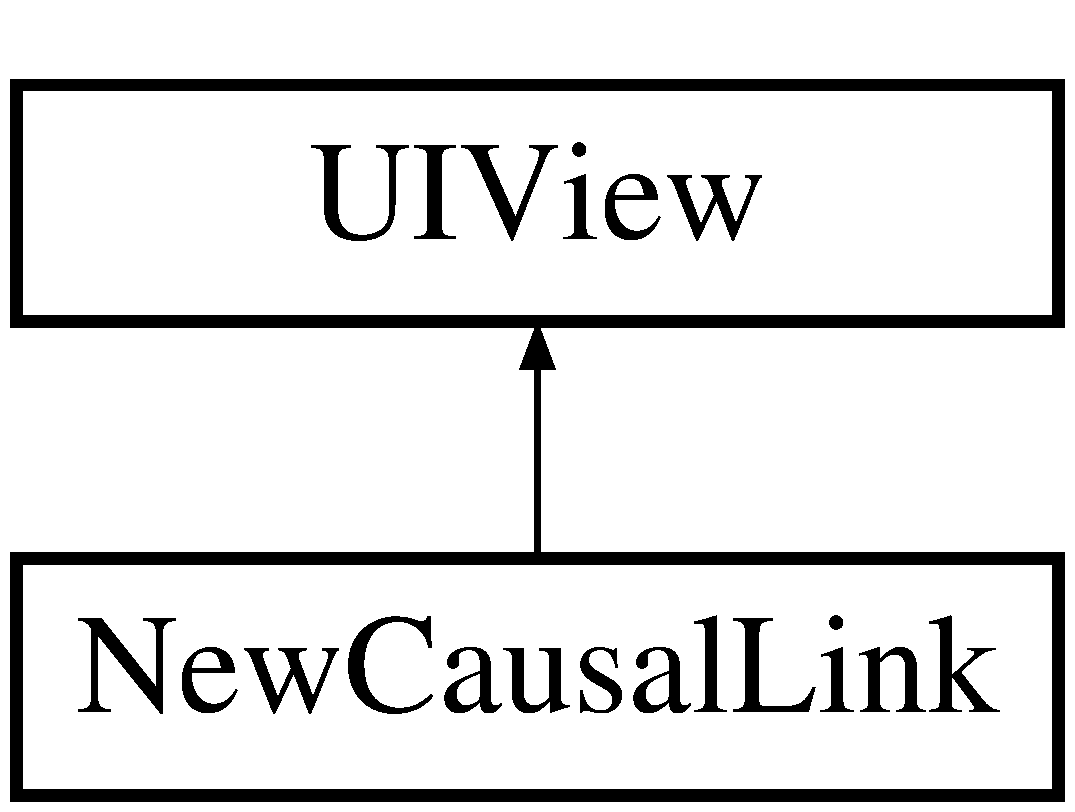
\includegraphics[height=2.000000cm]{interface_new_causal_link}
\end{center}
\end{figure}
\subsection*{Instance Methods}
\begin{DoxyCompactItemize}
\item 
(id) -\/ \hyperlink{interface_new_causal_link_a100c2da2d92d7d9a4da9ad851dcc1114}{init\-With\-Frame\-:}
\item 
(void) -\/ \hyperlink{interface_new_causal_link_a8c03538769a6fcbd7aa8e672cf4b5c96}{draw\-Rect\-:}
\end{DoxyCompactItemize}
\subsection*{Properties}
\begin{DoxyCompactItemize}
\item 
\hypertarget{interface_new_causal_link_af5c8aa466e345adfab2e58ba5509edad}{C\-G\-Point \hyperlink{interface_new_causal_link_af5c8aa466e345adfab2e58ba5509edad}{start\-Point}}\label{interface_new_causal_link_af5c8aa466e345adfab2e58ba5509edad}

\begin{DoxyCompactList}\small\item\em The starting point of the line. \end{DoxyCompactList}\item 
\hypertarget{interface_new_causal_link_a8182eda9bbf2964ae5df72b56cabffb0}{C\-G\-Point \hyperlink{interface_new_causal_link_a8182eda9bbf2964ae5df72b56cabffb0}{end\-Point}}\label{interface_new_causal_link_a8182eda9bbf2964ae5df72b56cabffb0}

\begin{DoxyCompactList}\small\item\em The ending point of the line. \end{DoxyCompactList}\end{DoxyCompactItemize}


\subsection{Detailed Description}
Creates the temporary line that represents where the link is going to connect to variables. This is used only when the user is dragging a new link from one variable to a new one. 

\subsection{Method Documentation}
\hypertarget{interface_new_causal_link_a8c03538769a6fcbd7aa8e672cf4b5c96}{\index{New\-Causal\-Link@{New\-Causal\-Link}!draw\-Rect\-:@{draw\-Rect\-:}}
\index{draw\-Rect\-:@{draw\-Rect\-:}!NewCausalLink@{New\-Causal\-Link}}
\subsubsection[{draw\-Rect\-:}]{\setlength{\rightskip}{0pt plus 5cm}-\/ (void) draw\-Rect\-: 
\begin{DoxyParamCaption}
\item[{(C\-G\-Rect)}]{rect}
\end{DoxyParamCaption}
}}\label{interface_new_causal_link_a8c03538769a6fcbd7aa8e672cf4b5c96}
Draws the receiver’s image within the passed-\/in rectangle. This is an overridden method. 
\begin{DoxyParams}{Parameters}
{\em rect} & the frame of the view in which objects can be drawn. \\
\hline
\end{DoxyParams}
\hypertarget{interface_new_causal_link_a100c2da2d92d7d9a4da9ad851dcc1114}{\index{New\-Causal\-Link@{New\-Causal\-Link}!init\-With\-Frame\-:@{init\-With\-Frame\-:}}
\index{init\-With\-Frame\-:@{init\-With\-Frame\-:}!NewCausalLink@{New\-Causal\-Link}}
\subsubsection[{init\-With\-Frame\-:}]{\setlength{\rightskip}{0pt plus 5cm}-\/ (id) init\-With\-Frame\-: 
\begin{DoxyParamCaption}
\item[{(C\-G\-Rect)}]{frame}
\end{DoxyParamCaption}
}}\label{interface_new_causal_link_a100c2da2d92d7d9a4da9ad851dcc1114}
Initializes the view. 
\begin{DoxyParams}{Parameters}
{\em frame} & the frame the view is contained within. \\
\hline
\end{DoxyParams}
\begin{DoxyReturn}{Returns}
an id of the newly created view 
\end{DoxyReturn}


The documentation for this class was generated from the following files\-:\begin{DoxyCompactItemize}
\item 
Group\-Modeling\-App/New\-Causal\-Link.\-h\item 
Group\-Modeling\-App/New\-Causal\-Link.\-m\end{DoxyCompactItemize}

\hypertarget{interface_reachability}{\section{Reachability Class Reference}
\label{interface_reachability}\index{Reachability@{Reachability}}
}
Inheritance diagram for Reachability\-:\begin{figure}[H]
\begin{center}
\leavevmode
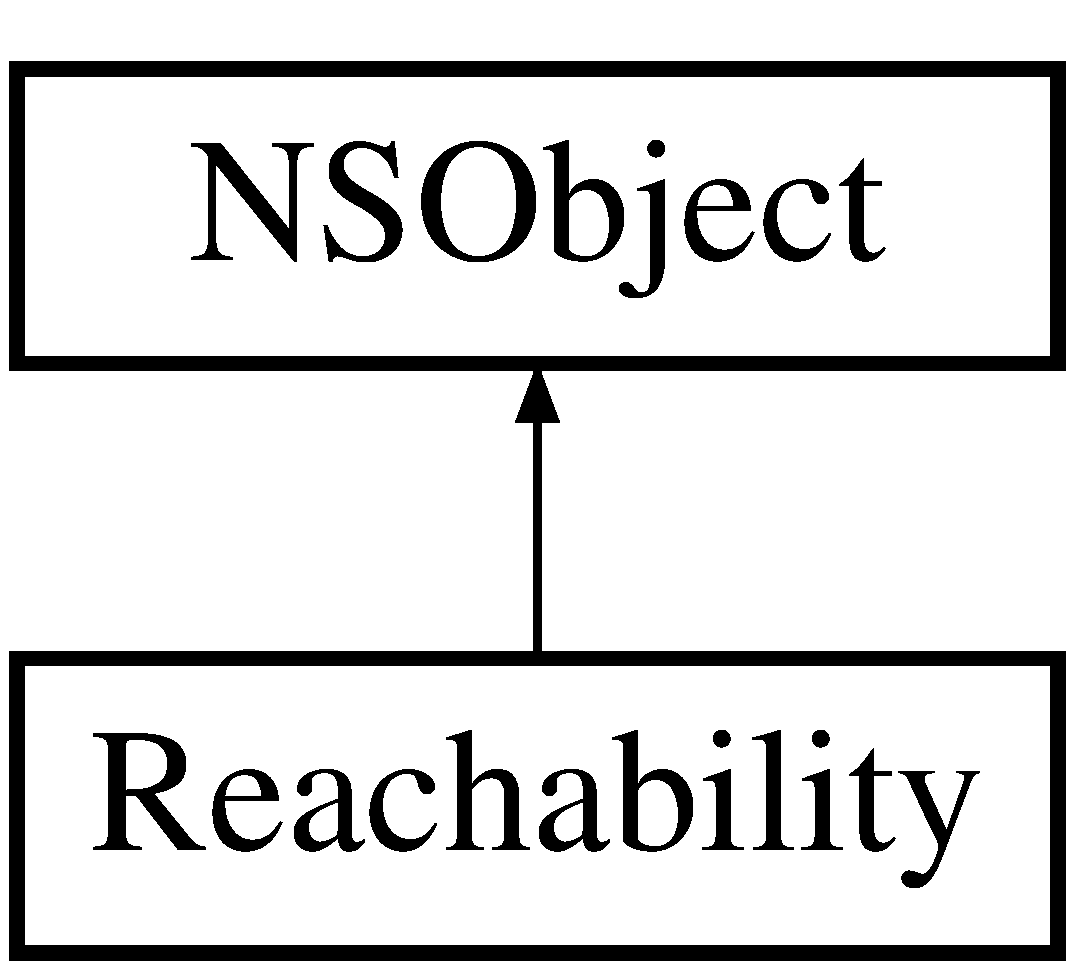
\includegraphics[height=2.000000cm]{interface_reachability}
\end{center}
\end{figure}
\subsection*{Instance Methods}
\begin{DoxyCompactItemize}
\item 
(B\-O\-O\-L) -\/ \hyperlink{interface_reachability_ab41a66b8c9a31c7164d7f67aa6026dfe}{start\-Notifier}
\item 
\hypertarget{interface_reachability_a78eccfa191bccad1d2f031906187aa63}{(void) -\/ {\bfseries stop\-Notifier}}\label{interface_reachability_a78eccfa191bccad1d2f031906187aa63}

\item 
\hypertarget{interface_reachability_a2ad5c5d8658d989648117c3b4b87b7d7}{(Network\-Status) -\/ {\bfseries current\-Reachability\-Status}}\label{interface_reachability_a2ad5c5d8658d989648117c3b4b87b7d7}

\item 
(B\-O\-O\-L) -\/ \hyperlink{interface_reachability_acbfea5cbb2bd94433fff2d814ac93028}{connection\-Required}
\end{DoxyCompactItemize}
\subsection*{Class Methods}
\begin{DoxyCompactItemize}
\item 
(instancetype) + \hyperlink{interface_reachability_a15adbd9589e5801d083aa9ef00ef3c80}{reachability\-With\-Host\-Name\-:}
\item 
(instancetype) + \hyperlink{interface_reachability_a773327c58a639c8c4ab9fec9ddcc0cd3}{reachability\-With\-Address\-:}
\item 
(instancetype) + \hyperlink{interface_reachability_a5854a2f4b1d1971459cace9ca9619b09}{reachability\-For\-Internet\-Connection}
\item 
(instancetype) + \hyperlink{interface_reachability_aead23497f0e9d4df9000549b3c258c1d}{reachability\-For\-Local\-Wi\-Fi}
\end{DoxyCompactItemize}


\subsection{Method Documentation}
\hypertarget{interface_reachability_acbfea5cbb2bd94433fff2d814ac93028}{\index{Reachability@{Reachability}!connection\-Required@{connection\-Required}}
\index{connection\-Required@{connection\-Required}!Reachability@{Reachability}}
\subsubsection[{connection\-Required}]{\setlength{\rightskip}{0pt plus 5cm}-\/ (B\-O\-O\-L) connection\-Required 
\begin{DoxyParamCaption}
{}
\end{DoxyParamCaption}
}}\label{interface_reachability_acbfea5cbb2bd94433fff2d814ac93028}
W\-W\-A\-N may be available, but not active until a connection has been established. Wi\-Fi may require a connection for V\-P\-N on Demand. \hypertarget{interface_reachability_a5854a2f4b1d1971459cace9ca9619b09}{\index{Reachability@{Reachability}!reachability\-For\-Internet\-Connection@{reachability\-For\-Internet\-Connection}}
\index{reachability\-For\-Internet\-Connection@{reachability\-For\-Internet\-Connection}!Reachability@{Reachability}}
\subsubsection[{reachability\-For\-Internet\-Connection}]{\setlength{\rightskip}{0pt plus 5cm}+ (instancetype) reachability\-For\-Internet\-Connection 
\begin{DoxyParamCaption}
{}
\end{DoxyParamCaption}
}}\label{interface_reachability_a5854a2f4b1d1971459cace9ca9619b09}
Checks whether the default route is available. Should be used by applications that do not connect to a particular host. \hypertarget{interface_reachability_aead23497f0e9d4df9000549b3c258c1d}{\index{Reachability@{Reachability}!reachability\-For\-Local\-Wi\-Fi@{reachability\-For\-Local\-Wi\-Fi}}
\index{reachability\-For\-Local\-Wi\-Fi@{reachability\-For\-Local\-Wi\-Fi}!Reachability@{Reachability}}
\subsubsection[{reachability\-For\-Local\-Wi\-Fi}]{\setlength{\rightskip}{0pt plus 5cm}+ (instancetype) reachability\-For\-Local\-Wi\-Fi 
\begin{DoxyParamCaption}
{}
\end{DoxyParamCaption}
}}\label{interface_reachability_aead23497f0e9d4df9000549b3c258c1d}
Checks whether a local Wi\-Fi connection is available. \hypertarget{interface_reachability_a773327c58a639c8c4ab9fec9ddcc0cd3}{\index{Reachability@{Reachability}!reachability\-With\-Address\-:@{reachability\-With\-Address\-:}}
\index{reachability\-With\-Address\-:@{reachability\-With\-Address\-:}!Reachability@{Reachability}}
\subsubsection[{reachability\-With\-Address\-:}]{\setlength{\rightskip}{0pt plus 5cm}+ (instancetype) reachability\-With\-Address\-: 
\begin{DoxyParamCaption}
\item[{(const struct sockaddr\-\_\-in $\ast$)}]{host\-Address}
\end{DoxyParamCaption}
}}\label{interface_reachability_a773327c58a639c8c4ab9fec9ddcc0cd3}
Use to check the reachability of a given I\-P address. \hypertarget{interface_reachability_a15adbd9589e5801d083aa9ef00ef3c80}{\index{Reachability@{Reachability}!reachability\-With\-Host\-Name\-:@{reachability\-With\-Host\-Name\-:}}
\index{reachability\-With\-Host\-Name\-:@{reachability\-With\-Host\-Name\-:}!Reachability@{Reachability}}
\subsubsection[{reachability\-With\-Host\-Name\-:}]{\setlength{\rightskip}{0pt plus 5cm}+ (instancetype) reachability\-With\-Host\-Name\-: 
\begin{DoxyParamCaption}
\item[{(N\-S\-String $\ast$)}]{host\-Name}
\end{DoxyParamCaption}
}}\label{interface_reachability_a15adbd9589e5801d083aa9ef00ef3c80}
Use to check the reachability of a given host name. \hypertarget{interface_reachability_ab41a66b8c9a31c7164d7f67aa6026dfe}{\index{Reachability@{Reachability}!start\-Notifier@{start\-Notifier}}
\index{start\-Notifier@{start\-Notifier}!Reachability@{Reachability}}
\subsubsection[{start\-Notifier}]{\setlength{\rightskip}{0pt plus 5cm}-\/ (B\-O\-O\-L) start\-Notifier 
\begin{DoxyParamCaption}
{}
\end{DoxyParamCaption}
}}\label{interface_reachability_ab41a66b8c9a31c7164d7f67aa6026dfe}
Start listening for reachability notifications on the current run loop. 

The documentation for this class was generated from the following files\-:\begin{DoxyCompactItemize}
\item 
Group\-Modeling\-App/Reachability.\-h\item 
Group\-Modeling\-App/Reachability.\-m\end{DoxyCompactItemize}

\hypertarget{interface_side_menu_view_controller}{\section{Side\-Menu\-View\-Controller Class Reference}
\label{interface_side_menu_view_controller}\index{Side\-Menu\-View\-Controller@{Side\-Menu\-View\-Controller}}
}


A view controller that handles the side menu bar.  




{\ttfamily \#import $<$Side\-Menu\-View\-Controller.\-h$>$}

Inheritance diagram for Side\-Menu\-View\-Controller\-:\begin{figure}[H]
\begin{center}
\leavevmode
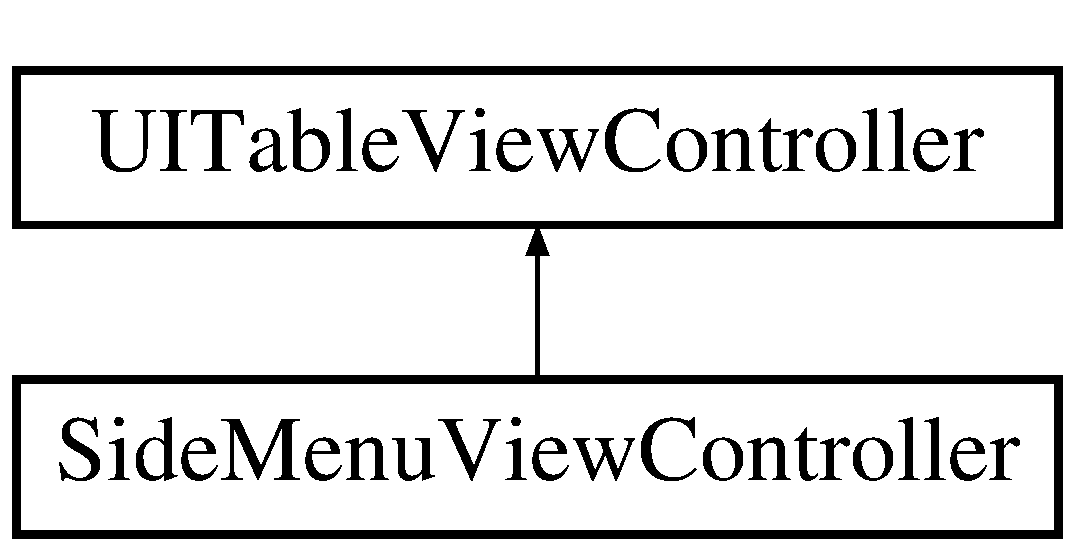
\includegraphics[height=2.000000cm]{interface_side_menu_view_controller}
\end{center}
\end{figure}
\subsection*{Instance Methods}
\begin{DoxyCompactItemize}
\item 
(\hyperlink{interface_m_f_side_menu_container_view_controller}{M\-F\-Side\-Menu\-Container\-View\-Controller} $\ast$) -\/ \hyperlink{interface_side_menu_view_controller_ad9f497773e1c2f5e420929a60f3bf7df}{menu\-Container\-View\-Controller}
\item 
(id) -\/ \hyperlink{interface_side_menu_view_controller_a4213bb26f5207ee3f402fe463badc691}{init}
\item 
\hypertarget{interface_side_menu_view_controller_a2c868393a6f59adcf2a8973ca95d631b}{(void) -\/ \hyperlink{interface_side_menu_view_controller_a2c868393a6f59adcf2a8973ca95d631b}{load\-Database}}\label{interface_side_menu_view_controller_a2c868393a6f59adcf2a8973ca95d631b}

\begin{DoxyCompactList}\small\item\em Loads the menu items. \end{DoxyCompactList}\item 
(N\-S\-String $\ast$) -\/ \hyperlink{interface_side_menu_view_controller_a5757190cb856a85c44de064864982f27}{table\-View\-:title\-For\-Header\-In\-Section\-:}
\item 
(N\-S\-Integer) -\/ \hyperlink{interface_side_menu_view_controller_a06b0471f3085f21304b18e41c6bfac6f}{number\-Of\-Sections\-In\-Table\-View\-:}
\item 
(N\-S\-Integer) -\/ \hyperlink{interface_side_menu_view_controller_aab440a4915232be470a3170a94dc5c82}{table\-View\-:number\-Of\-Rows\-In\-Section\-:}
\item 
(U\-I\-Table\-View\-Cell $\ast$) -\/ \hyperlink{interface_side_menu_view_controller_a8b22b55c4ff90cc2a2a96f2a38695ffe}{table\-View\-:cell\-For\-Row\-At\-Index\-Path\-:}
\item 
(void) -\/ \hyperlink{interface_side_menu_view_controller_a6741a2fd8b94b02a8b6adb99b30ba7d1}{table\-View\-:did\-Select\-Row\-At\-Index\-Path\-:}
\end{DoxyCompactItemize}
\subsection*{Protected Attributes}
\begin{DoxyCompactItemize}
\item 
\hypertarget{interface_side_menu_view_controller_a90224d9e597665265fbf07aac6847cc5}{N\-S\-Mutable\-Array $\ast$ {\bfseries menu\-Options}}\label{interface_side_menu_view_controller_a90224d9e597665265fbf07aac6847cc5}

\end{DoxyCompactItemize}


\subsection{Detailed Description}
A view controller that handles the side menu bar. 

\subsection{Method Documentation}
\hypertarget{interface_side_menu_view_controller_a4213bb26f5207ee3f402fe463badc691}{\index{Side\-Menu\-View\-Controller@{Side\-Menu\-View\-Controller}!init@{init}}
\index{init@{init}!SideMenuViewController@{Side\-Menu\-View\-Controller}}
\subsubsection[{init}]{\setlength{\rightskip}{0pt plus 5cm}-\/ (id) init 
\begin{DoxyParamCaption}
{}
\end{DoxyParamCaption}
}}\label{interface_side_menu_view_controller_a4213bb26f5207ee3f402fe463badc691}
Initializes the view controller. 
\begin{DoxyParams}{Parameters}
{\em style} & the style of the view controller. \\
\hline
\end{DoxyParams}
\begin{DoxyReturn}{Returns}
an id of the newly created view controller. 
\end{DoxyReturn}
\hypertarget{interface_side_menu_view_controller_ad9f497773e1c2f5e420929a60f3bf7df}{\index{Side\-Menu\-View\-Controller@{Side\-Menu\-View\-Controller}!menu\-Container\-View\-Controller@{menu\-Container\-View\-Controller}}
\index{menu\-Container\-View\-Controller@{menu\-Container\-View\-Controller}!SideMenuViewController@{Side\-Menu\-View\-Controller}}
\subsubsection[{menu\-Container\-View\-Controller}]{\setlength{\rightskip}{0pt plus 5cm}-\/ ({\bf M\-F\-Side\-Menu\-Container\-View\-Controller} $\ast$) menu\-Container\-View\-Controller 
\begin{DoxyParamCaption}
{}
\end{DoxyParamCaption}
}}\label{interface_side_menu_view_controller_ad9f497773e1c2f5e420929a60f3bf7df}
Gets the menu container view controller. \begin{DoxyReturn}{Returns}
the menu container view controller. 
\end{DoxyReturn}
\hypertarget{interface_side_menu_view_controller_a06b0471f3085f21304b18e41c6bfac6f}{\index{Side\-Menu\-View\-Controller@{Side\-Menu\-View\-Controller}!number\-Of\-Sections\-In\-Table\-View\-:@{number\-Of\-Sections\-In\-Table\-View\-:}}
\index{number\-Of\-Sections\-In\-Table\-View\-:@{number\-Of\-Sections\-In\-Table\-View\-:}!SideMenuViewController@{Side\-Menu\-View\-Controller}}
\subsubsection[{number\-Of\-Sections\-In\-Table\-View\-:}]{\setlength{\rightskip}{0pt plus 5cm}-\/ (N\-S\-Integer) number\-Of\-Sections\-In\-Table\-View\-: 
\begin{DoxyParamCaption}
\item[{(U\-I\-Table\-View $\ast$)}]{table\-View}
\end{DoxyParamCaption}
}}\label{interface_side_menu_view_controller_a06b0471f3085f21304b18e41c6bfac6f}
Returns the number of sections in the table view. 
\begin{DoxyParams}{Parameters}
{\em table\-View} & the reference table view. \\
\hline
\end{DoxyParams}
\begin{DoxyReturn}{Returns}
the number of the sections in the table view. 
\end{DoxyReturn}
\hypertarget{interface_side_menu_view_controller_a8b22b55c4ff90cc2a2a96f2a38695ffe}{\index{Side\-Menu\-View\-Controller@{Side\-Menu\-View\-Controller}!table\-View\-:cell\-For\-Row\-At\-Index\-Path\-:@{table\-View\-:cell\-For\-Row\-At\-Index\-Path\-:}}
\index{table\-View\-:cell\-For\-Row\-At\-Index\-Path\-:@{table\-View\-:cell\-For\-Row\-At\-Index\-Path\-:}!SideMenuViewController@{Side\-Menu\-View\-Controller}}
\subsubsection[{table\-View\-:cell\-For\-Row\-At\-Index\-Path\-:}]{\setlength{\rightskip}{0pt plus 5cm}-\/ (U\-I\-Table\-View\-Cell $\ast$) table\-View\-: 
\begin{DoxyParamCaption}
\item[{(U\-I\-Table\-View $\ast$)}]{table\-View}
\item[{cellForRowAtIndexPath:(N\-S\-Index\-Path $\ast$)}]{index\-Path}
\end{DoxyParamCaption}
}}\label{interface_side_menu_view_controller_a8b22b55c4ff90cc2a2a96f2a38695ffe}
Sets the label text of the cell based on what is contained in the database. 
\begin{DoxyParams}{Parameters}
{\em table\-View} & the reference table view. \\
\hline
{\em index\-Path} & the index path that contains where in the list you are. \\
\hline
\end{DoxyParams}
\begin{DoxyReturn}{Returns}
the newly created/reused cell. 
\end{DoxyReturn}
\hypertarget{interface_side_menu_view_controller_a6741a2fd8b94b02a8b6adb99b30ba7d1}{\index{Side\-Menu\-View\-Controller@{Side\-Menu\-View\-Controller}!table\-View\-:did\-Select\-Row\-At\-Index\-Path\-:@{table\-View\-:did\-Select\-Row\-At\-Index\-Path\-:}}
\index{table\-View\-:did\-Select\-Row\-At\-Index\-Path\-:@{table\-View\-:did\-Select\-Row\-At\-Index\-Path\-:}!SideMenuViewController@{Side\-Menu\-View\-Controller}}
\subsubsection[{table\-View\-:did\-Select\-Row\-At\-Index\-Path\-:}]{\setlength{\rightskip}{0pt plus 5cm}-\/ (void) table\-View\-: 
\begin{DoxyParamCaption}
\item[{(U\-I\-Table\-View $\ast$)}]{table\-View}
\item[{didSelectRowAtIndexPath:(N\-S\-Index\-Path $\ast$)}]{index\-Path}
\end{DoxyParamCaption}
}}\label{interface_side_menu_view_controller_a6741a2fd8b94b02a8b6adb99b30ba7d1}
Will update the view that is showing when a new menu option is selected. 
\begin{DoxyParams}{Parameters}
{\em table\-View} & the reference table view. \\
\hline
{\em index\-Path} & the index path that contains where in the list you are. \\
\hline
\end{DoxyParams}
\hypertarget{interface_side_menu_view_controller_aab440a4915232be470a3170a94dc5c82}{\index{Side\-Menu\-View\-Controller@{Side\-Menu\-View\-Controller}!table\-View\-:number\-Of\-Rows\-In\-Section\-:@{table\-View\-:number\-Of\-Rows\-In\-Section\-:}}
\index{table\-View\-:number\-Of\-Rows\-In\-Section\-:@{table\-View\-:number\-Of\-Rows\-In\-Section\-:}!SideMenuViewController@{Side\-Menu\-View\-Controller}}
\subsubsection[{table\-View\-:number\-Of\-Rows\-In\-Section\-:}]{\setlength{\rightskip}{0pt plus 5cm}-\/ (N\-S\-Integer) table\-View\-: 
\begin{DoxyParamCaption}
\item[{(U\-I\-Table\-View $\ast$)}]{table\-View}
\item[{numberOfRowsInSection:(N\-S\-Integer)}]{section}
\end{DoxyParamCaption}
}}\label{interface_side_menu_view_controller_aab440a4915232be470a3170a94dc5c82}
Returns the number of rows in a section in the table view. 
\begin{DoxyParams}{Parameters}
{\em table\-View} & the reference table view. \\
\hline
{\em section} & the current section of the table view. \\
\hline
\end{DoxyParams}
\begin{DoxyReturn}{Returns}
the number of the sections in the table view. 
\end{DoxyReturn}
\hypertarget{interface_side_menu_view_controller_a5757190cb856a85c44de064864982f27}{\index{Side\-Menu\-View\-Controller@{Side\-Menu\-View\-Controller}!table\-View\-:title\-For\-Header\-In\-Section\-:@{table\-View\-:title\-For\-Header\-In\-Section\-:}}
\index{table\-View\-:title\-For\-Header\-In\-Section\-:@{table\-View\-:title\-For\-Header\-In\-Section\-:}!SideMenuViewController@{Side\-Menu\-View\-Controller}}
\subsubsection[{table\-View\-:title\-For\-Header\-In\-Section\-:}]{\setlength{\rightskip}{0pt plus 5cm}-\/ (N\-S\-String $\ast$) table\-View\-: 
\begin{DoxyParamCaption}
\item[{(U\-I\-Table\-View $\ast$)}]{table\-View}
\item[{titleForHeaderInSection:(N\-S\-Integer)}]{section}
\end{DoxyParamCaption}
}}\label{interface_side_menu_view_controller_a5757190cb856a85c44de064864982f27}
Returns the title of the section header for the table. 
\begin{DoxyParams}{Parameters}
{\em table\-View} & the reference table view. \\
\hline
{\em section} & the integer representing the section. \\
\hline
\end{DoxyParams}
\begin{DoxyReturn}{Returns}
a string values to set for the header title. 
\end{DoxyReturn}


The documentation for this class was generated from the following files\-:\begin{DoxyCompactItemize}
\item 
Group\-Modeling\-App/Side\-Menu\-View\-Controller.\-h\item 
Group\-Modeling\-App/Side\-Menu\-View\-Controller.\-m\end{DoxyCompactItemize}

\hypertarget{interface_variable}{\section{Variable Class Reference}
\label{interface_variable}\index{Variable@{Variable}}
}


A subclass of \hyperlink{interface_component}{Component} containing the data related to a variable of a causal loop diagram. ex. In a diagram on Childhood obesity, \char`\"{}\-Fast Food\char`\"{} may be a variable in the model influencing childhood obesity.  




{\ttfamily \#import $<$Variable.\-h$>$}

Inheritance diagram for Variable\-:\begin{figure}[H]
\begin{center}
\leavevmode
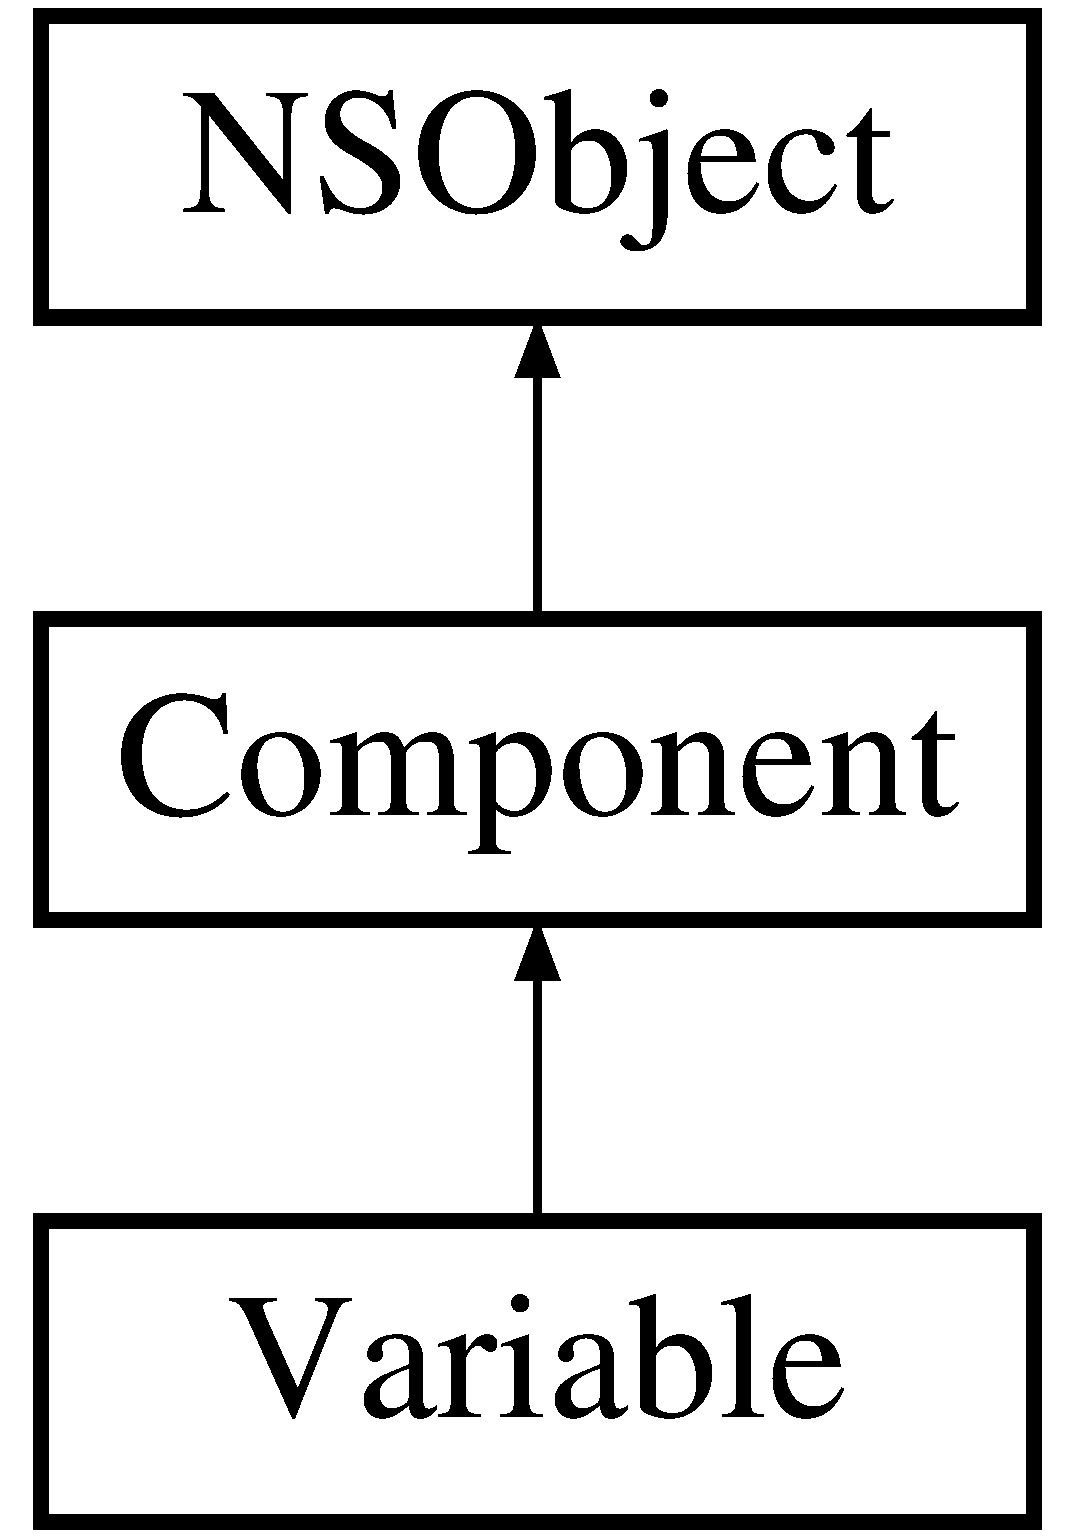
\includegraphics[height=3.000000cm]{interface_variable}
\end{center}
\end{figure}
\subsection*{Instance Methods}
\begin{DoxyCompactItemize}
\item 
(void) -\/ \hyperlink{interface_variable_a94f7b8f580fb81fe04cbdb35e5058336}{add\-Indegree\-Link\-:}
\item 
(void) -\/ \hyperlink{interface_variable_ae0173c90b0ab12d38f7ad61696ed8e54}{add\-Outdegree\-Link\-:}
\item 
(id) -\/ \hyperlink{interface_variable_ae3fdc3a923d3d3be4b4aeb821cb90734}{init\-:}
\item 
(id) -\/ \hyperlink{interface_variable_a9755af4c66523c228c80713cab6396fe}{init\-With\-Location\-:}
\item 
(int) -\/ \hyperlink{interface_variable_a79b759708a8f8644dd6913b4ae5762e5}{get\-Variable\-Height}
\item 
(int) -\/ \hyperlink{interface_variable_a388e832a7faf40b36f9a7a6f592d58d7}{get\-Variable\-Width}
\item 
(void) -\/ \hyperlink{interface_variable_a36d0d6828a9b4691b0db41445af18317}{remove\-Indgree\-Link\-:}
\item 
(void) -\/ \hyperlink{interface_variable_a025b64b058ba0294e2ef0bf10cbc70e7}{remove\-Outdgree\-Link\-:}
\item 
(N\-S\-Array $\ast$) -\/ \hyperlink{interface_variable_a1ff5e4a4052dff234ff327980ae2f92e}{create\-Var\-Map}
\item 
(N\-S\-String $\ast$) -\/ \hyperlink{interface_variable_a4c7e0685f86eef33404c7ada436db10a}{create\-Variable\-Output\-String}
\end{DoxyCompactItemize}
\subsection*{Properties}
\begin{DoxyCompactItemize}
\item 
\hypertarget{interface_variable_acccd26f3cbfd25fc87ff63a9e5ebd6cf}{N\-S\-Mutable\-Array $\ast$ \hyperlink{interface_variable_acccd26f3cbfd25fc87ff63a9e5ebd6cf}{indegree\-Links}}\label{interface_variable_acccd26f3cbfd25fc87ff63a9e5ebd6cf}

\begin{DoxyCompactList}\small\item\em An array of \hyperlink{interface_causal_link}{Causal\-Link} objects that point to this variable. \end{DoxyCompactList}\item 
\hypertarget{interface_variable_aafe54a40e314c1bb23ea7d5cb5456586}{N\-S\-Mutable\-Array $\ast$ \hyperlink{interface_variable_aafe54a40e314c1bb23ea7d5cb5456586}{outdegree\-Links}}\label{interface_variable_aafe54a40e314c1bb23ea7d5cb5456586}

\begin{DoxyCompactList}\small\item\em An array of \hyperlink{interface_causal_link}{Causal\-Link} objects that extend from this variable. \end{DoxyCompactList}\item 
\hypertarget{interface_variable_a0e3597199260a059ec632e5d54adb06e}{int \hyperlink{interface_variable_a0e3597199260a059ec632e5d54adb06e}{text\-Position}}\label{interface_variable_a0e3597199260a059ec632e5d54adb06e}

\begin{DoxyCompactList}\small\item\em Where the text holding the variable name is located in relation to the variable object. \end{DoxyCompactList}\item 
\hypertarget{interface_variable_a7e8a4af98b5a08b166ccd5d637cb380a}{\hyperlink{interface_variable_view}{Variable\-View} $\ast$ \hyperlink{interface_variable_a7e8a4af98b5a08b166ccd5d637cb380a}{view}}\label{interface_variable_a7e8a4af98b5a08b166ccd5d637cb380a}

\begin{DoxyCompactList}\small\item\em The U\-I\-View that will contain the graphical representation of the variable. \end{DoxyCompactList}\end{DoxyCompactItemize}
\subsection*{Additional Inherited Members}


\subsection{Detailed Description}
A subclass of \hyperlink{interface_component}{Component} containing the data related to a variable of a causal loop diagram. ex. In a diagram on Childhood obesity, \char`\"{}\-Fast Food\char`\"{} may be a variable in the model influencing childhood obesity. 

\subsection{Method Documentation}
\hypertarget{interface_variable_a94f7b8f580fb81fe04cbdb35e5058336}{\index{Variable@{Variable}!add\-Indegree\-Link\-:@{add\-Indegree\-Link\-:}}
\index{add\-Indegree\-Link\-:@{add\-Indegree\-Link\-:}!Variable@{Variable}}
\subsubsection[{add\-Indegree\-Link\-:}]{\setlength{\rightskip}{0pt plus 5cm}-\/ (void) add\-Indegree\-Link\-: 
\begin{DoxyParamCaption}
\item[{(id)}]{link}
\end{DoxyParamCaption}
}}\label{interface_variable_a94f7b8f580fb81fe04cbdb35e5058336}
Add a \hyperlink{interface_causal_link}{Causal\-Link} to the list of indegree links to this variable. 
\begin{DoxyParams}{Parameters}
{\em link} & the \hyperlink{interface_causal_link}{Causal\-Link} that should be added. \\
\hline
\end{DoxyParams}
\hypertarget{interface_variable_ae0173c90b0ab12d38f7ad61696ed8e54}{\index{Variable@{Variable}!add\-Outdegree\-Link\-:@{add\-Outdegree\-Link\-:}}
\index{add\-Outdegree\-Link\-:@{add\-Outdegree\-Link\-:}!Variable@{Variable}}
\subsubsection[{add\-Outdegree\-Link\-:}]{\setlength{\rightskip}{0pt plus 5cm}-\/ (void) add\-Outdegree\-Link\-: 
\begin{DoxyParamCaption}
\item[{(id)}]{link}
\end{DoxyParamCaption}
}}\label{interface_variable_ae0173c90b0ab12d38f7ad61696ed8e54}
Add a \hyperlink{interface_causal_link}{Causal\-Link} to the list of outdegree links to this variable. 
\begin{DoxyParams}{Parameters}
{\em link} & the \hyperlink{interface_causal_link}{Causal\-Link} that should be added. \\
\hline
\end{DoxyParams}
\hypertarget{interface_variable_a4c7e0685f86eef33404c7ada436db10a}{\index{Variable@{Variable}!create\-Variable\-Output\-String@{create\-Variable\-Output\-String}}
\index{create\-Variable\-Output\-String@{create\-Variable\-Output\-String}!Variable@{Variable}}
\subsubsection[{create\-Variable\-Output\-String}]{\setlength{\rightskip}{0pt plus 5cm}-\/ (N\-S\-String $\ast$) create\-Variable\-Output\-String 
\begin{DoxyParamCaption}
{}
\end{DoxyParamCaption}
}}\label{interface_variable_a4c7e0685f86eef33404c7ada436db10a}
Constructs the output string for a \hyperlink{interface_variable}{Variable}. The string is constructed to be readable by Vensim. Follows the string pattern\-: \mbox{[}Object Type\mbox{]},\mbox{[}Object id\mbox{]},\mbox{[}Object Name\mbox{]},\mbox{[}X Location\mbox{]},\mbox{[}Y Location\mbox{]},?,?,\mbox{[}\hyperlink{interface_variable}{Variable} Type\mbox{]},3,0,0,\mbox{[}Text Position\mbox{]},0,0,0 \begin{DoxyReturn}{Returns}
the string of data for the variable. 
\end{DoxyReturn}
\begin{DoxyRefDesc}{Todo}
\item[\hyperlink{todo__todo000004}{Todo}]I do not put the extra characters vensim uses for " \end{DoxyRefDesc}
\hypertarget{interface_variable_a1ff5e4a4052dff234ff327980ae2f92e}{\index{Variable@{Variable}!create\-Var\-Map@{create\-Var\-Map}}
\index{create\-Var\-Map@{create\-Var\-Map}!Variable@{Variable}}
\subsubsection[{create\-Var\-Map}]{\setlength{\rightskip}{0pt plus 5cm}-\/ (N\-S\-Array $\ast$) create\-Var\-Map 
\begin{DoxyParamCaption}
{}
\end{DoxyParamCaption}
}}\label{interface_variable_a1ff5e4a4052dff234ff327980ae2f92e}
Constructs the variable map, identifying which variables influence the current variable. Vensim constructs maps to display how the variables are related. Example of the output created\-: Big \hyperlink{interface_variable}{Variable} = A F\-U\-N\-C\-T\-I\-O\-N O\-F( variable 1,variable 2) $\sim$ $\sim$ $|$ \begin{DoxyReturn}{Returns}
an array that contains the three lines that represent the map for the variable. 
\end{DoxyReturn}
\hypertarget{interface_variable_a79b759708a8f8644dd6913b4ae5762e5}{\index{Variable@{Variable}!get\-Variable\-Height@{get\-Variable\-Height}}
\index{get\-Variable\-Height@{get\-Variable\-Height}!Variable@{Variable}}
\subsubsection[{get\-Variable\-Height}]{\setlength{\rightskip}{0pt plus 5cm}-\/ (int) get\-Variable\-Height 
\begin{DoxyParamCaption}
{}
\end{DoxyParamCaption}
}}\label{interface_variable_a79b759708a8f8644dd6913b4ae5762e5}
Gets the height of the variable view. \begin{DoxyReturn}{Returns}
the height of the variable view. 
\end{DoxyReturn}
\hypertarget{interface_variable_a388e832a7faf40b36f9a7a6f592d58d7}{\index{Variable@{Variable}!get\-Variable\-Width@{get\-Variable\-Width}}
\index{get\-Variable\-Width@{get\-Variable\-Width}!Variable@{Variable}}
\subsubsection[{get\-Variable\-Width}]{\setlength{\rightskip}{0pt plus 5cm}-\/ (int) get\-Variable\-Width 
\begin{DoxyParamCaption}
{}
\end{DoxyParamCaption}
}}\label{interface_variable_a388e832a7faf40b36f9a7a6f592d58d7}
Gets the width of the variable view. \begin{DoxyReturn}{Returns}
the width of the variable view. 
\end{DoxyReturn}
\hypertarget{interface_variable_ae3fdc3a923d3d3be4b4aeb821cb90734}{\index{Variable@{Variable}!init\-:@{init\-:}}
\index{init\-:@{init\-:}!Variable@{Variable}}
\subsubsection[{init\-:}]{\setlength{\rightskip}{0pt plus 5cm}-\/ (id) init\-: 
\begin{DoxyParamCaption}
\item[{(N\-S\-Array$\ast$)}]{data}
\end{DoxyParamCaption}
}}\label{interface_variable_ae3fdc3a923d3d3be4b4aeb821cb90734}
Initializes the \hyperlink{interface_variable}{Variable} when you are loading data from a mdl file. 
\begin{DoxyParams}{Parameters}
{\em data} & an array of strings containing all of the data for the variable from a Vensim mdl file. \\
\hline
\end{DoxyParams}
\begin{DoxyReturn}{Returns}
a pointer to the newly created \hyperlink{interface_variable}{Variable}. 
\end{DoxyReturn}
\hypertarget{interface_variable_a9755af4c66523c228c80713cab6396fe}{\index{Variable@{Variable}!init\-With\-Location\-:@{init\-With\-Location\-:}}
\index{init\-With\-Location\-:@{init\-With\-Location\-:}!Variable@{Variable}}
\subsubsection[{init\-With\-Location\-:}]{\setlength{\rightskip}{0pt plus 5cm}-\/ (id) init\-With\-Location\-: 
\begin{DoxyParamCaption}
\item[{(C\-G\-Point)}]{location}
\end{DoxyParamCaption}
}}\label{interface_variable_a9755af4c66523c228c80713cab6396fe}
Initizlizes the \hyperlink{interface_variable}{Variable} when you are adding a brand new variable. 
\begin{DoxyParams}{Parameters}
{\em location} & the location of the new object in the frame. \\
\hline
\end{DoxyParams}
\begin{DoxyReturn}{Returns}
a pointer to the newly created \hyperlink{interface_variable}{Variable}. 
\end{DoxyReturn}
\hypertarget{interface_variable_a36d0d6828a9b4691b0db41445af18317}{\index{Variable@{Variable}!remove\-Indgree\-Link\-:@{remove\-Indgree\-Link\-:}}
\index{remove\-Indgree\-Link\-:@{remove\-Indgree\-Link\-:}!Variable@{Variable}}
\subsubsection[{remove\-Indgree\-Link\-:}]{\setlength{\rightskip}{0pt plus 5cm}-\/ (void) remove\-Indgree\-Link\-: 
\begin{DoxyParamCaption}
\item[{(id)}]{link}
\end{DoxyParamCaption}
}}\label{interface_variable_a36d0d6828a9b4691b0db41445af18317}
Removes a \hyperlink{interface_causal_link}{Causal\-Link} from the list of indegree links for this variable. 
\begin{DoxyParams}{Parameters}
{\em link} & the \hyperlink{interface_causal_link}{Causal\-Link} that should be deleted. \\
\hline
\end{DoxyParams}
\hypertarget{interface_variable_a025b64b058ba0294e2ef0bf10cbc70e7}{\index{Variable@{Variable}!remove\-Outdgree\-Link\-:@{remove\-Outdgree\-Link\-:}}
\index{remove\-Outdgree\-Link\-:@{remove\-Outdgree\-Link\-:}!Variable@{Variable}}
\subsubsection[{remove\-Outdgree\-Link\-:}]{\setlength{\rightskip}{0pt plus 5cm}-\/ (void) remove\-Outdgree\-Link\-: 
\begin{DoxyParamCaption}
\item[{(id)}]{link}
\end{DoxyParamCaption}
}}\label{interface_variable_a025b64b058ba0294e2ef0bf10cbc70e7}
Removes a \hyperlink{interface_causal_link}{Causal\-Link} from the list of outdegree links for this variable. 
\begin{DoxyParams}{Parameters}
{\em link} & the \hyperlink{interface_causal_link}{Causal\-Link} that should be deleted. \\
\hline
\end{DoxyParams}


The documentation for this class was generated from the following files\-:\begin{DoxyCompactItemize}
\item 
Group\-Modeling\-App/Variable.\-h\item 
Group\-Modeling\-App/Variable.\-m\end{DoxyCompactItemize}

\hypertarget{interface_variable_edit_menu_view}{\section{Variable\-Edit\-Menu\-View Class Reference}
\label{interface_variable_edit_menu_view}\index{Variable\-Edit\-Menu\-View@{Variable\-Edit\-Menu\-View}}
}


The view that will contain the edit menu for Variables.  




{\ttfamily \#import $<$Variable\-Edit\-Menu\-View.\-h$>$}

Inheritance diagram for Variable\-Edit\-Menu\-View\-:\begin{figure}[H]
\begin{center}
\leavevmode
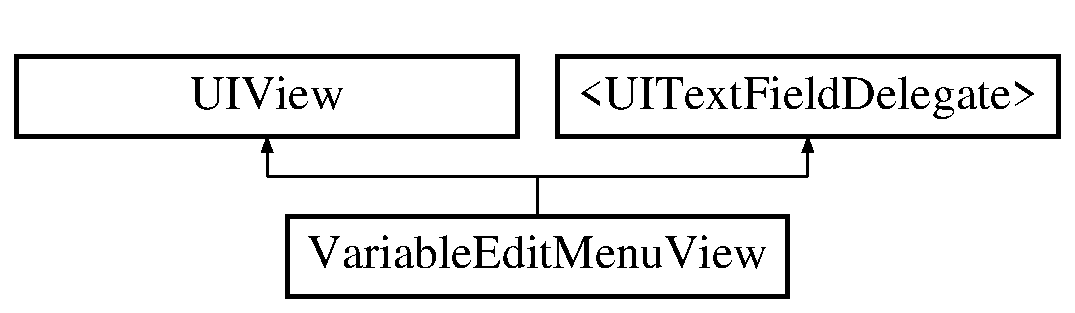
\includegraphics[height=2.000000cm]{interface_variable_edit_menu_view}
\end{center}
\end{figure}
\subsection*{Instance Methods}
\begin{DoxyCompactItemize}
\item 
(id) -\/ \hyperlink{interface_variable_edit_menu_view_ad1475d40e606d4f009f89321944e3678}{init\-With\-Frame\-:view\-:}
\item 
\hypertarget{interface_variable_edit_menu_view_aa9f8d1d0bae6f6dd7ef7269d1c2fbe30}{(void) -\/ \hyperlink{interface_variable_edit_menu_view_aa9f8d1d0bae6f6dd7ef7269d1c2fbe30}{type\-Control\-Change}}\label{interface_variable_edit_menu_view_aa9f8d1d0bae6f6dd7ef7269d1c2fbe30}

\begin{DoxyCompactList}\small\item\em Notifies the logger when a new option from the type segmented control has been changed. \end{DoxyCompactList}\item 
\hypertarget{interface_variable_edit_menu_view_a6bd6409bbc288f769683443ae909a4ad}{(void) -\/ \hyperlink{interface_variable_edit_menu_view_a6bd6409bbc288f769683443ae909a4ad}{update\-Variable}}\label{interface_variable_edit_menu_view_a6bd6409bbc288f769683443ae909a4ad}

\begin{DoxyCompactList}\small\item\em This method will be called when the save button is called to save the attributes. \end{DoxyCompactList}\item 
(void) -\/ \hyperlink{interface_variable_edit_menu_view_ac9394b979597f8df8e15f5abc1cc7a2e}{text\-Field\-Did\-Begin\-Editing\-:}
\item 
(void) -\/ \hyperlink{interface_variable_edit_menu_view_aa7337263d1e997c99cdc506fc61dcea3}{text\-Field\-Did\-End\-Editing\-:}
\item 
(B\-O\-O\-L) -\/ \hyperlink{interface_variable_edit_menu_view_a1a8ec9c257f3a894dc9b3389477f55e9}{text\-Field\-Should\-Return\-:}
\end{DoxyCompactItemize}
\subsection*{Properties}
\begin{DoxyCompactItemize}
\item 
\hypertarget{interface_variable_edit_menu_view_af91fc4ee7ce5ce8ac3b0f00e38824b04}{U\-I\-Label $\ast$ \hyperlink{interface_variable_edit_menu_view_af91fc4ee7ce5ce8ac3b0f00e38824b04}{name\-Label}}\label{interface_variable_edit_menu_view_af91fc4ee7ce5ce8ac3b0f00e38824b04}

\begin{DoxyCompactList}\small\item\em The label that represents what name\-Text\-Field represents. \end{DoxyCompactList}\item 
\hypertarget{interface_variable_edit_menu_view_a5cbc9eaf5c10f7b61fa933746ae0bb6e}{U\-I\-Text\-Field $\ast$ \hyperlink{interface_variable_edit_menu_view_a5cbc9eaf5c10f7b61fa933746ae0bb6e}{name\-Text\-Field}}\label{interface_variable_edit_menu_view_a5cbc9eaf5c10f7b61fa933746ae0bb6e}

\begin{DoxyCompactList}\small\item\em The text field that contains the name of the object. \end{DoxyCompactList}\item 
\hypertarget{interface_variable_edit_menu_view_ad87205d9304809167df2212ab8f146e9}{\hyperlink{interface_variable_view}{Variable\-View} $\ast$ \hyperlink{interface_variable_edit_menu_view_ad87205d9304809167df2212ab8f146e9}{object\-View}}\label{interface_variable_edit_menu_view_ad87205d9304809167df2212ab8f146e9}

\begin{DoxyCompactList}\small\item\em The view of the object that you are editing. \end{DoxyCompactList}\item 
\hypertarget{interface_variable_edit_menu_view_a326ccc069e5a0781354c0cc85dc4550d}{U\-I\-Segmented\-Control $\ast$ \hyperlink{interface_variable_edit_menu_view_a326ccc069e5a0781354c0cc85dc4550d}{type\-Controls}}\label{interface_variable_edit_menu_view_a326ccc069e5a0781354c0cc85dc4550d}

\begin{DoxyCompactList}\small\item\em The segmented control that allows the user to change the type of variable. \end{DoxyCompactList}\item 
\hypertarget{interface_variable_edit_menu_view_af06d4a271255059c61da80cfc91f9835}{U\-I\-Label $\ast$ \hyperlink{interface_variable_edit_menu_view_af06d4a271255059c61da80cfc91f9835}{type\-Label}}\label{interface_variable_edit_menu_view_af06d4a271255059c61da80cfc91f9835}

\begin{DoxyCompactList}\small\item\em The label that represents what type\-Contols represents. \end{DoxyCompactList}\end{DoxyCompactItemize}


\subsection{Detailed Description}
The view that will contain the edit menu for Variables. 

\subsection{Method Documentation}
\hypertarget{interface_variable_edit_menu_view_ad1475d40e606d4f009f89321944e3678}{\index{Variable\-Edit\-Menu\-View@{Variable\-Edit\-Menu\-View}!init\-With\-Frame\-:view\-:@{init\-With\-Frame\-:view\-:}}
\index{init\-With\-Frame\-:view\-:@{init\-With\-Frame\-:view\-:}!VariableEditMenuView@{Variable\-Edit\-Menu\-View}}
\subsubsection[{init\-With\-Frame\-:view\-:}]{\setlength{\rightskip}{0pt plus 5cm}-\/ (id) init\-With\-Frame\-: 
\begin{DoxyParamCaption}
\item[{(C\-G\-Rect)}]{frame}
\item[{view:(U\-I\-View$\ast$)}]{view}
\end{DoxyParamCaption}
}}\label{interface_variable_edit_menu_view_ad1475d40e606d4f009f89321944e3678}
Initializes the view. 
\begin{DoxyParams}{Parameters}
{\em frame} & the frame the view is contained within. \\
\hline
\end{DoxyParams}
\begin{DoxyReturn}{Returns}
an id of the newly created view. 
\end{DoxyReturn}
\hypertarget{interface_variable_edit_menu_view_ac9394b979597f8df8e15f5abc1cc7a2e}{\index{Variable\-Edit\-Menu\-View@{Variable\-Edit\-Menu\-View}!text\-Field\-Did\-Begin\-Editing\-:@{text\-Field\-Did\-Begin\-Editing\-:}}
\index{text\-Field\-Did\-Begin\-Editing\-:@{text\-Field\-Did\-Begin\-Editing\-:}!VariableEditMenuView@{Variable\-Edit\-Menu\-View}}
\subsubsection[{text\-Field\-Did\-Begin\-Editing\-:}]{\setlength{\rightskip}{0pt plus 5cm}-\/ (void) text\-Field\-Did\-Begin\-Editing\-: 
\begin{DoxyParamCaption}
\item[{(U\-I\-Text\-Field $\ast$)}]{text\-Field}
\end{DoxyParamCaption}
}}\label{interface_variable_edit_menu_view_ac9394b979597f8df8e15f5abc1cc7a2e}
Will log when the keyboard opens up for the user to edit. 
\begin{DoxyParams}{Parameters}
{\em text\-Field} & the textfield that makes the call. \\
\hline
\end{DoxyParams}
\hypertarget{interface_variable_edit_menu_view_aa7337263d1e997c99cdc506fc61dcea3}{\index{Variable\-Edit\-Menu\-View@{Variable\-Edit\-Menu\-View}!text\-Field\-Did\-End\-Editing\-:@{text\-Field\-Did\-End\-Editing\-:}}
\index{text\-Field\-Did\-End\-Editing\-:@{text\-Field\-Did\-End\-Editing\-:}!VariableEditMenuView@{Variable\-Edit\-Menu\-View}}
\subsubsection[{text\-Field\-Did\-End\-Editing\-:}]{\setlength{\rightskip}{0pt plus 5cm}-\/ (void) text\-Field\-Did\-End\-Editing\-: 
\begin{DoxyParamCaption}
\item[{(U\-I\-Text\-Field $\ast$)}]{text\-Field}
\end{DoxyParamCaption}
}}\label{interface_variable_edit_menu_view_aa7337263d1e997c99cdc506fc61dcea3}
Will log when the keyboard closes. Cannot place event in text\-Field\-Should\-Return becuase i\-O\-S 5 does not call the method. 
\begin{DoxyParams}{Parameters}
{\em text\-Field} & the textfield that makes the call. \\
\hline
\end{DoxyParams}
\hypertarget{interface_variable_edit_menu_view_a1a8ec9c257f3a894dc9b3389477f55e9}{\index{Variable\-Edit\-Menu\-View@{Variable\-Edit\-Menu\-View}!text\-Field\-Should\-Return\-:@{text\-Field\-Should\-Return\-:}}
\index{text\-Field\-Should\-Return\-:@{text\-Field\-Should\-Return\-:}!VariableEditMenuView@{Variable\-Edit\-Menu\-View}}
\subsubsection[{text\-Field\-Should\-Return\-:}]{\setlength{\rightskip}{0pt plus 5cm}-\/ (B\-O\-O\-L) text\-Field\-Should\-Return\-: 
\begin{DoxyParamCaption}
\item[{(U\-I\-Text\-Field $\ast$)}]{text\-Field}
\end{DoxyParamCaption}
}}\label{interface_variable_edit_menu_view_a1a8ec9c257f3a894dc9b3389477f55e9}
Determines whether the keyboard should close for the text field. 
\begin{DoxyParams}{Parameters}
{\em text\-Field} & the textfield that makes the call. \\
\hline
\end{DoxyParams}
\begin{DoxyReturn}{Returns}
will always be true and the keyboard will always close when the Done button is pressed. 
\end{DoxyReturn}


The documentation for this class was generated from the following files\-:\begin{DoxyCompactItemize}
\item 
Group\-Modeling\-App/Variable\-Edit\-Menu\-View.\-h\item 
Group\-Modeling\-App/Variable\-Edit\-Menu\-View.\-m\end{DoxyCompactItemize}

\hypertarget{interface_variable_view}{\section{Variable\-View Class Reference}
\label{interface_variable_view}\index{Variable\-View@{Variable\-View}}
}


The view that will contain the graphical representation of a \hyperlink{interface_variable}{Variable}.  




{\ttfamily \#import $<$Variable\-View.\-h$>$}

Inheritance diagram for Variable\-View\-:\begin{figure}[H]
\begin{center}
\leavevmode
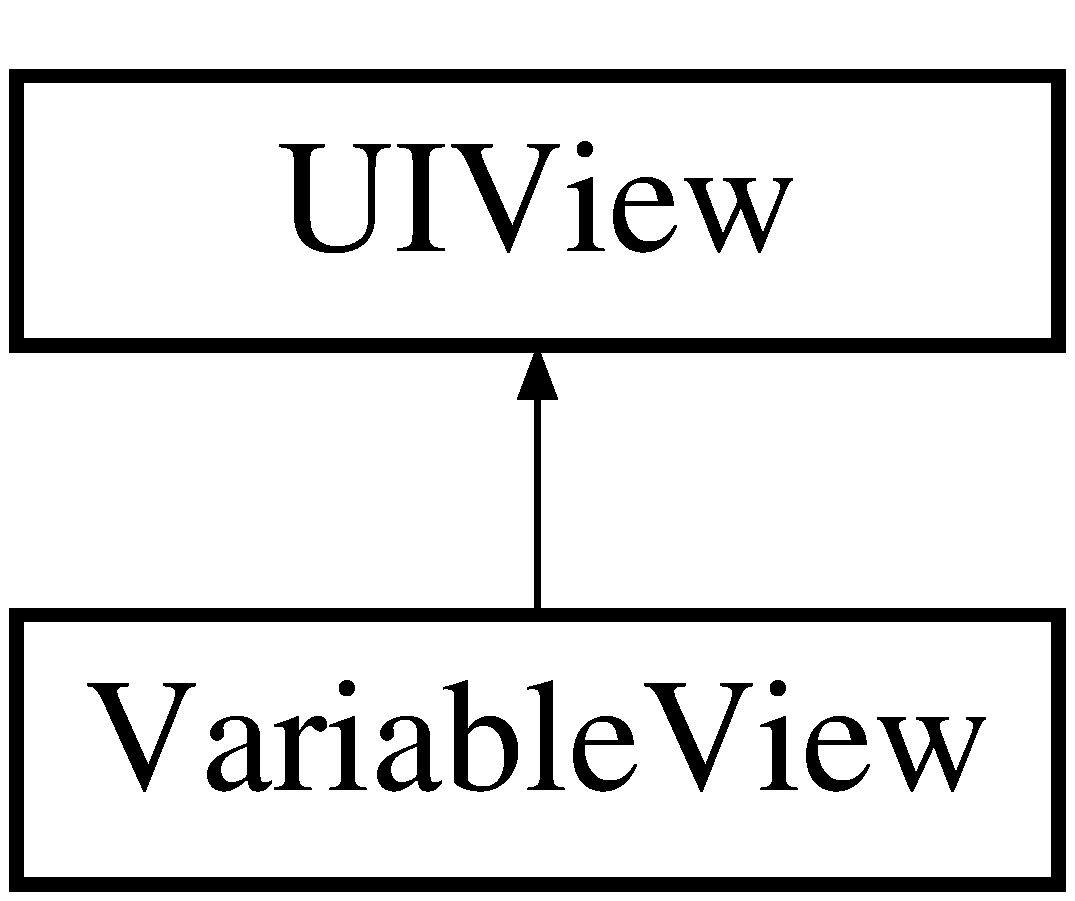
\includegraphics[height=2.000000cm]{interface_variable_view}
\end{center}
\end{figure}
\subsection*{Instance Methods}
\begin{DoxyCompactItemize}
\item 
(id) -\/ \hyperlink{interface_variable_view_a1e7227b1d41e651a603e80315935a3ee}{init\-With\-Frame\-:and\-Parent\-:}
\item 
(void) -\/ \hyperlink{interface_variable_view_a8c03538769a6fcbd7aa8e672cf4b5c96}{draw\-Rect\-:}
\item 
(void) -\/ \hyperlink{interface_variable_view_a2357112d7fefe9f720ac82c881236830}{touches\-Began\-:with\-Event\-:}
\item 
(void) -\/ \hyperlink{interface_variable_view_a06bf1152e9fa0dd16bf7f46128ae0cff}{touches\-Moved\-:with\-Event\-:}
\item 
(void) -\/ \hyperlink{interface_variable_view_ad9cc995e0aa0c5e28ab827a06c897c36}{touches\-Ended\-:with\-Event\-:}
\item 
(void) -\/ \hyperlink{interface_variable_view_a38393b10eebe5376725616eb446df377}{handle\-Single\-Tap\-:}
\item 
(void) -\/ \hyperlink{interface_variable_view_ae1e3768fefe8a80686d2be0a8e21472f}{long\-Press\-Detected\-:}
\item 
(void) -\/ \hyperlink{interface_variable_view_abde0ec8a6fa1e0d26aa777c67b12dcac}{set\-Box\-Color\-Based\-On\-Point\-:}
\end{DoxyCompactItemize}
\subsection*{Properties}
\begin{DoxyCompactItemize}
\item 
\hypertarget{interface_variable_view_adffdfe6d544463a4ec27f62889403aa4}{U\-I\-Color $\ast$ \hyperlink{interface_variable_view_adffdfe6d544463a4ec27f62889403aa4}{box\-Color}}\label{interface_variable_view_adffdfe6d544463a4ec27f62889403aa4}

\begin{DoxyCompactList}\small\item\em The color of the variable box. Used when creating new causal links. \end{DoxyCompactList}\item 
\hypertarget{interface_variable_view_a8eccf963342a358cf524a44e0696771e}{bool \hyperlink{interface_variable_view_a8eccf963342a358cf524a44e0696771e}{is\-Boxed}}\label{interface_variable_view_a8eccf963342a358cf524a44e0696771e}

\begin{DoxyCompactList}\small\item\em Whether the variable is boxed. \end{DoxyCompactList}\item 
\hypertarget{interface_variable_view_a4b93d352d2fca75b34e1b5a50e03f587}{N\-S\-String $\ast$ \hyperlink{interface_variable_view_a4b93d352d2fca75b34e1b5a50e03f587}{name}}\label{interface_variable_view_a4b93d352d2fca75b34e1b5a50e03f587}

\begin{DoxyCompactList}\small\item\em The name of the variable. \end{DoxyCompactList}\item 
\hypertarget{interface_variable_view_a4376b99467d16ed71554a4a6ddd4ae0a}{id \hyperlink{interface_variable_view_a4376b99467d16ed71554a4a6ddd4ae0a}{parent}}\label{interface_variable_view_a4376b99467d16ed71554a4a6ddd4ae0a}

\begin{DoxyCompactList}\small\item\em Pointer to the parent of this view. \end{DoxyCompactList}\item 
\hypertarget{interface_variable_view_ab9596dece716623542ebe46b3abda05b}{\hyperlink{interface_new_causal_link}{New\-Causal\-Link} $\ast$ \hyperlink{interface_variable_view_ab9596dece716623542ebe46b3abda05b}{temp\-Link}}\label{interface_variable_view_ab9596dece716623542ebe46b3abda05b}

\begin{DoxyCompactList}\small\item\em An instance of \hyperlink{interface_new_causal_link}{New\-Causal\-Link} which is used when creating a new causal link. \end{DoxyCompactList}\end{DoxyCompactItemize}


\subsection{Detailed Description}
The view that will contain the graphical representation of a \hyperlink{interface_variable}{Variable}. 

\subsection{Method Documentation}
\hypertarget{interface_variable_view_a8c03538769a6fcbd7aa8e672cf4b5c96}{\index{Variable\-View@{Variable\-View}!draw\-Rect\-:@{draw\-Rect\-:}}
\index{draw\-Rect\-:@{draw\-Rect\-:}!VariableView@{Variable\-View}}
\subsubsection[{draw\-Rect\-:}]{\setlength{\rightskip}{0pt plus 5cm}-\/ (void) draw\-Rect\-: 
\begin{DoxyParamCaption}
\item[{(C\-G\-Rect)}]{rect}
\end{DoxyParamCaption}
}}\label{interface_variable_view_a8c03538769a6fcbd7aa8e672cf4b5c96}
Draws the receiver’s image within the passed-\/in rectangle. This is an overridden method. 
\begin{DoxyParams}{Parameters}
{\em rect} & the frame of the view in which objects can be drawn. \\
\hline
\end{DoxyParams}
\hypertarget{interface_variable_view_a38393b10eebe5376725616eb446df377}{\index{Variable\-View@{Variable\-View}!handle\-Single\-Tap\-:@{handle\-Single\-Tap\-:}}
\index{handle\-Single\-Tap\-:@{handle\-Single\-Tap\-:}!VariableView@{Variable\-View}}
\subsubsection[{handle\-Single\-Tap\-:}]{\setlength{\rightskip}{0pt plus 5cm}-\/ (void) handle\-Single\-Tap\-: 
\begin{DoxyParamCaption}
\item[{(U\-I\-Tap\-Gesture\-Recognizer $\ast$)}]{sender}
\end{DoxyParamCaption}
}}\label{interface_variable_view_a38393b10eebe5376725616eb446df377}
Will open up the menu of options for the object on a single tap. 
\begin{DoxyParams}{Parameters}
{\em sender} & the recognizer that fired the method call. \\
\hline
\end{DoxyParams}
\hypertarget{interface_variable_view_a1e7227b1d41e651a603e80315935a3ee}{\index{Variable\-View@{Variable\-View}!init\-With\-Frame\-:and\-Parent\-:@{init\-With\-Frame\-:and\-Parent\-:}}
\index{init\-With\-Frame\-:and\-Parent\-:@{init\-With\-Frame\-:and\-Parent\-:}!VariableView@{Variable\-View}}
\subsubsection[{init\-With\-Frame\-:and\-Parent\-:}]{\setlength{\rightskip}{0pt plus 5cm}-\/ (id) init\-With\-Frame\-: 
\begin{DoxyParamCaption}
\item[{(C\-G\-Rect)}]{frame}
\item[{andParent:(id)}]{parent}
\end{DoxyParamCaption}
}}\label{interface_variable_view_a1e7227b1d41e651a603e80315935a3ee}
Initializes the view. 
\begin{DoxyParams}{Parameters}
{\em frame} & the frame the view is contained within. \\
\hline
{\em parent} & a pointer to the parent object that holds the view. \\
\hline
\end{DoxyParams}
\begin{DoxyReturn}{Returns}
an id of the newly created view 
\end{DoxyReturn}
\hypertarget{interface_variable_view_ae1e3768fefe8a80686d2be0a8e21472f}{\index{Variable\-View@{Variable\-View}!long\-Press\-Detected\-:@{long\-Press\-Detected\-:}}
\index{long\-Press\-Detected\-:@{long\-Press\-Detected\-:}!VariableView@{Variable\-View}}
\subsubsection[{long\-Press\-Detected\-:}]{\setlength{\rightskip}{0pt plus 5cm}-\/ (void) long\-Press\-Detected\-: 
\begin{DoxyParamCaption}
\item[{(U\-I\-Long\-Press\-Gesture\-Recognizer$\ast$)}]{sender}
\end{DoxyParamCaption}
}}\label{interface_variable_view_ae1e3768fefe8a80686d2be0a8e21472f}
The long press is used to determine when a user wants to add a new causal\-Link. A user can only add a causal\-Link from clicking on a variable. 
\begin{DoxyParams}{Parameters}
{\em sender} & the recognizer that fired the method call. \\
\hline
\end{DoxyParams}
\hypertarget{interface_variable_view_abde0ec8a6fa1e0d26aa777c67b12dcac}{\index{Variable\-View@{Variable\-View}!set\-Box\-Color\-Based\-On\-Point\-:@{set\-Box\-Color\-Based\-On\-Point\-:}}
\index{set\-Box\-Color\-Based\-On\-Point\-:@{set\-Box\-Color\-Based\-On\-Point\-:}!VariableView@{Variable\-View}}
\subsubsection[{set\-Box\-Color\-Based\-On\-Point\-:}]{\setlength{\rightskip}{0pt plus 5cm}-\/ (void) set\-Box\-Color\-Based\-On\-Point\-: 
\begin{DoxyParamCaption}
\item[{(C\-G\-Point)}]{point}
\end{DoxyParamCaption}
}}\label{interface_variable_view_abde0ec8a6fa1e0d26aa777c67b12dcac}
Will set the color of the frame based on a point. If the provided point falls within the bounds of the variable, the color will be different than if the point does not lie within the bounds. This method is used to highlight variables when the user is trying to add new causal links. 
\begin{DoxyParams}{Parameters}
{\em point} & the reference point to determine what the color of the view should be. \\
\hline
\end{DoxyParams}
\hypertarget{interface_variable_view_a2357112d7fefe9f720ac82c881236830}{\index{Variable\-View@{Variable\-View}!touches\-Began\-:with\-Event\-:@{touches\-Began\-:with\-Event\-:}}
\index{touches\-Began\-:with\-Event\-:@{touches\-Began\-:with\-Event\-:}!VariableView@{Variable\-View}}
\subsubsection[{touches\-Began\-:with\-Event\-:}]{\setlength{\rightskip}{0pt plus 5cm}-\/ (void) touches\-Began\-: 
\begin{DoxyParamCaption}
\item[{(N\-S\-Set $\ast$)}]{touches}
\item[{withEvent:(U\-I\-Event $\ast$)}]{event}
\end{DoxyParamCaption}
}}\label{interface_variable_view_a2357112d7fefe9f720ac82c881236830}
Logs event at the beginning of moving the variable. 
\begin{DoxyParams}{Parameters}
{\em touches} & the set of touch events registered by the application. \\
\hline
{\em event} & the U\-I\-Event that fired the the method call. \\
\hline
\end{DoxyParams}
\hypertarget{interface_variable_view_ad9cc995e0aa0c5e28ab827a06c897c36}{\index{Variable\-View@{Variable\-View}!touches\-Ended\-:with\-Event\-:@{touches\-Ended\-:with\-Event\-:}}
\index{touches\-Ended\-:with\-Event\-:@{touches\-Ended\-:with\-Event\-:}!VariableView@{Variable\-View}}
\subsubsection[{touches\-Ended\-:with\-Event\-:}]{\setlength{\rightskip}{0pt plus 5cm}-\/ (void) touches\-Ended\-: 
\begin{DoxyParamCaption}
\item[{(N\-S\-Set $\ast$)}]{touches}
\item[{withEvent:(U\-I\-Event $\ast$)}]{event}
\end{DoxyParamCaption}
}}\label{interface_variable_view_ad9cc995e0aa0c5e28ab827a06c897c36}
Logs event at the end of moving the variable. 
\begin{DoxyParams}{Parameters}
{\em touches} & the set of touch events registered by the application. \\
\hline
{\em event} & the U\-I\-Event that fired the the method call. \\
\hline
\end{DoxyParams}
\hypertarget{interface_variable_view_a06bf1152e9fa0dd16bf7f46128ae0cff}{\index{Variable\-View@{Variable\-View}!touches\-Moved\-:with\-Event\-:@{touches\-Moved\-:with\-Event\-:}}
\index{touches\-Moved\-:with\-Event\-:@{touches\-Moved\-:with\-Event\-:}!VariableView@{Variable\-View}}
\subsubsection[{touches\-Moved\-:with\-Event\-:}]{\setlength{\rightskip}{0pt plus 5cm}-\/ (void) touches\-Moved\-: 
\begin{DoxyParamCaption}
\item[{(N\-S\-Set $\ast$)}]{touches}
\item[{withEvent:(U\-I\-Event $\ast$)}]{event}
\end{DoxyParamCaption}
}}\label{interface_variable_view_a06bf1152e9fa0dd16bf7f46128ae0cff}
Handles moving the variable object across the view when the user drags the object 
\begin{DoxyParams}{Parameters}
{\em touches} & the set of touch events registered by the application \\
\hline
{\em event} & the U\-I\-Event that fired the the method call \\
\hline
\end{DoxyParams}


The documentation for this class was generated from the following files\-:\begin{DoxyCompactItemize}
\item 
Group\-Modeling\-App/Variable\-View.\-h\item 
Group\-Modeling\-App/Variable\-View.\-m\end{DoxyCompactItemize}

%--- End generated contents ---

% Index
\newpage
\phantomsection
\addcontentsline{toc}{part}{Index}
\printindex

\end{document}
